% **************************************************
% Document Class Definition
% **************************************************
\documentclass[%
    paper=A4,               % paper size --> A4 is default in Germany
    twoside=true,           % onesite or twoside printing
    openright,              % doublepage cleaning ends up right side
    parskip=full,           % spacing value / method for paragraphs
    chapterprefix=true,     % prefix for chapter marks
    12pt,                   % font size
    headings=normal,        % size of headings
    bibliography=totoc,     % include bib in toc
    listof=totoc,           % include listof entries in toc
    titlepage=on,           % own page for each title page
    captions=tableabove,    % display table captions above the float env
    draft=false            % value for draft version
]{scrreprt}%


% **************************************************
% Setup YOUR thesis document in this file !
% **************************************************
% !TEX root = thesis.tex


% **************************************************
% Files' Character Encoding
% **************************************************
\PassOptionsToPackage{utf8}{inputenc}
\usepackage{inputenc}


% **************************************************
% Information and Commands for Reuse
% **************************************************
\newcommand{\thesisTitle}{One-shot recognition for art historic images}
\newcommand{\thesisName}{Maurice Frank}
\newcommand{\thesisSubject}{Documentation}
\newcommand{\thesisDate}{May 17, 2017}
\newcommand{\thesisVersion}{v1.0}

\newcommand{\thesisFirstReviewer}{Björn Ommer}
\newcommand{\thesisFirstReviewerUniversity}{\protect{University of Heidelberg}}
\newcommand{\thesisFirstReviewerDepartment}{Department of Mathematics and Computer Science}

\newcommand{\thesisSecondReviewer}{John Doe}
\newcommand{\thesisSecondReviewerUniversity}{\protect{University of Heidelberg}}
\newcommand{\thesisSecondReviewerDepartment}{Department of Mathematics and Computer Science}

\newcommand{\thesisFirstSupervisor}{Miguel Angel Bautista}

\newcommand{\thesisUniversity}{\protect{University of Heidelberg}}
\newcommand{\thesisUniversityDepartment}{Department of Mathematics and Computer Science}
\newcommand{\thesisUniversityInstitute}{Heidelberg Collaboratory for Image Processing}
\newcommand{\thesisUniversityGroup}{Computer Vision Research Group}
\newcommand{\thesisUniversityCity}{Heidelberg}
\newcommand{\thesisUniversityStreetAddress}{Berliner Str. 43}
\newcommand{\thesisUniversityPostalCode}{69120}


% **************************************************
% Debug LaTeX Information
% **************************************************
%\listfiles


% **************************************************
% Load and Configure Packages
% **************************************************
\usepackage[english]{babel} % babel system, adjust the language of the content
\PassOptionsToPackage{% setup clean thesis style
    figuresep=colon,%
    sansserif=false,%
    hangfigurecaption=false,%
    hangsection=true,%
    hangsubsection=true,%
    colorize=full,%
    colortheme=redyellow,%
    bibsys=biber,%
    bibfile=assets/references,%
    bibstyle=alphabetic,%
    wrapfooter=false,%
}{cleanthesis}
\usepackage{cleanthesis}

\hypersetup{% setup the hyperref-package options
    pdftitle={\thesisTitle},    %   - title (PDF meta)
    pdfsubject={\thesisSubject},%   - subject (PDF meta)
    pdfauthor={\thesisName},    %   - author (PDF meta)
    plainpages=false,           %   -
    colorlinks=false,           %   - colorize links?
    pdfborder={0 0 0},          %   -
    breaklinks=true,            %   - allow line break inside links
    bookmarksnumbered=true,     %
    bookmarksopen=true          %
}

\usepackage[xindy, toc]{glossaries}
\makeglossaries
\newacronym{fcn}{FCN}{Fully Convolutional Network}
\newacronym{resnet}{ResNet}{Residual Network}
\newacronym{relu}{ReLu}{Rectified Linear Unit}
\newacronym{fc}{FC}{Fully Connected}

\newglossaryentry{conv}{
    name={Conv},
    description={Convolution}
}


\usepackage{tikz}
\usetikzlibrary{arrows,chains,matrix,positioning,scopes}

\newcommand{\bigO}[1]{$\mathcal{O}(#1)$}
\newcommand{\rocplot}[1]{\includegraphics[width=0.47\textwidth]{figures/ppart_results/#1_roc.pdf}}
\newcommand{\prplot}[1]{\includegraphics[width=0.47\textwidth]{figures/ppart_results/#1_precs_recs.pdf}}
\newcommand{\appim}[1]{\includegraphics[height=2cm]{figures/app/#1}}
\newcommand{\hmim}[1]{\includegraphics[height=1.7cm]{figures/hm_examples/#1}}


\usepackage{multirow}



% **************************************************
% Document CONTENT
% **************************************************
\begin{document}

% --------------------------
% rename document parts
% --------------------------
%\renewcaptionname{ngerman}{\figurename}{Abb.}
%\renewcaptionname{ngerman}{\tablename}{Tab.}
\renewcaptionname{english}{\figurename}{Fig.}
\renewcaptionname{english}{\tablename}{Tab.}

% --------------------------
% Front matter
% --------------------------
\pagenumbering{roman}			% roman page numbing (invisible for empty page style)
\pagestyle{empty}				% no header or footers
% !TEX root = ../thesis.tex
%
% ------------------------------------  --> cover title page
\begin{titlepage}
	\pdfbookmark[0]{Cover}{Cover}
	\flushright
	\hfill
	\vfill
	{\Large\thesisTitleGerman \par}
	{\LARGE\thesisTitle \par}
	\rule[5pt]{\textwidth}{.4pt} \par
	{\Large\thesisName}
	\vfill
	\textit{\large\thesisDate} \\
\end{titlepage}


% ------------------------------------  --> main title page
\begin{titlepage}
	\pdfbookmark[0]{Titlepage}{Titlepage}
	\tgherosfont
	\centering

	{\Large \thesisUniversity} \\[4mm]
	\textsf{\thesisUniversityDepartment} \\
	\textsf{\thesisUniversityInstitute} \\
	\textsf{\thesisUniversityGroup} \\

	\vfill
	{\large \thesisSubject} \\[5mm]
	{\Large \color{ctcolortitle}\textbf{\thesisTitleGerman} \\[10mm]}
	{\LARGE \color{ctcolortitle}\textbf{\thesisTitle} \\[10mm]}
	{\Large \thesisName} \\
	{\large \thesisStudentID} \\

	\vfill
	\begin{minipage}[t]{.27\textwidth}
		\raggedleft
		\textit{Reviewer}
	\end{minipage}
	\hspace*{15pt}
	\begin{minipage}[t]{.65\textwidth}
		{\Large \thesisFirstReviewer} \\
	  	{\small \thesisFirstReviewerDepartment} \\[-1mm]
		{\small \thesisFirstReviewerUniversity}
	\end{minipage} \\[5mm]
	% \begin{minipage}[t]{.27\textwidth}
	% 	\raggedleft
	% 	\textit{2. Reviewer}
	% \end{minipage}
	% \hspace*{15pt}
	% \begin{minipage}[t]{.65\textwidth}
	% 	{\Large \thesisSecondReviewer} \\
	%   	{\small \thesisSecondReviewerDepartment} \\[-1mm]
	% 	{\small \thesisSecondReviewerUniversity}
	% \end{minipage} \\[10mm]
	\begin{minipage}[t]{.27\textwidth}
		\raggedleft
		\textit{Supervisors}
	\end{minipage}
	\hspace*{15pt}
	\begin{minipage}[t]{.65\textwidth}
		\thesisFirstSupervisor
	\end{minipage} \\[10mm]

	\thesisDate \\

\end{titlepage}


% ------------------------------------  --> lower title back for single page layout
\hfill
\vfill
{
	\small
	\textbf{\thesisName} \\
	\textit{\thesisTitle} \\
	\textit{\thesisTitleGerman} \\
	\thesisSubject, \thesisDate \\
	Reviewers: \thesisFirstReviewer\\ %\ and \thesisSecondReviewer \\
	Supervisors: \thesisFirstSupervisor \\[1.5em]
	\textbf{\thesisUniversity} \\
	\textit{\thesisUniversityGroup} \\
	\thesisUniversityInstitute \\
	\thesisUniversityDepartment \\
	\thesisUniversityStreetAddress \\
	\thesisUniversityPostalCode\ and \thesisUniversityCity
}
		% INCLUDE: all titlepages
\cleardoublepage

\pagestyle{plain}				% display just page numbers
% !TEX root = ../my-thesis.tex
%
\pdfbookmark[0]{Abstract}{Abstract}
\chapter*{Abstract}
\label{sec:abstract}
\vspace*{-10mm}

\blindtext

\vspace*{20mm}

{\usekomafont{chapter}Zusammenfassung}\label{sec:abstract-diff} \\

\blindtext
		% INCLUDE: the abstracts (english and german)
\cleardoublepage
%
\setcounter{tocdepth}{2}		% define depth of toc
\tableofcontents				% display table of contents
\cleardoublepage

% --------------------------
% Body matter
% --------------------------
\pagenumbering{arabic}			% arabic page numbering
\setcounter{page}{1}			% set page counter
\pagestyle{maincontentstyle} 	% fancy header and footer

% !TEX root = ../thesis.tex
%
\chapter{Introduction}
\label{sec:intro}
Today more and more work processes can be supported, or replaced through intelligent machines. Computer Vision proves itself capable of understanding images and video on a near-human level or even outperforming normal human capabilities in some visual tasks. One reason intelligent machines are absolutely needed today and in the future are the enormous masses of data the \textit{digital natives}, companies or scientists generate and store. Independent of the performance difference between computer and human, it its often impossible to work through catalogs or databases of millions or more images, music recordings, scientific data records et cetera. To automate such tasks does not only relieve from monotonous work but also enables humans to achieve more in less time.\\
At the very latest with the development of analog and digital mass storage systems scientists began to base their research on findings from mass data. No different scientists of the humanities move their work into a digital form. Being able to quickly look up any painting as a digital image or shifting through unique, in some archive locked, manuscripts from the middle ages makes drawing connections and research considerable easier. As we can assume these databases to grow or already have grown over any humans capabilities, digital humanities are a prime example for the application of visual learning and automation.

\section{Problem Statement}
\label{sec:intro:motivation}
For this thesis we approach one of possible applications of Computer Vision in the digital humanities, in particular art history. We assume a historian doing work on a huge set of digitized images $\mathbb{I}$. Those could be scans of medieval writings, architecture sketches or photos of historic paintings. The images are assumed to be not at all annotated meaning we do not have any metadata containing e.g. the creator.

Now the historian wants to compare all images $I = \{i_1, i_2,\dotsc,i_n\} \subset \mathbb{I}$ conjunct in-that they all share some visual pattern $p$, may it be they depict the same person or show all a similar scenery. We want to provide the user of this database a method to automatically generate the set $I$. This should be done giving a image $\tau$ which the historian states for, that it contains $p$. Therefore we need a function $C(i)$ which can decide for a image $i\in\mathbb{I}$ whether it possesses $p$ and therefore is part of the seeked set $I$. The only data we can use to adjust the operator $C$ is the sample image $\tau$.\\Proposing one approach for this $C_\tau$ and a generator function $G(\tau) = C_\tau$ is the problem of this thesis.

\section{Thesis Structure}
\label{sec:intro:structure}
The thesis is structured as follows. Firstly in \textbf{\treft{sec:concepts}} we give a quick overview over the topics and techniques used in this work including a short introduction to the inner workings of \glspl{cnn}. In \textbf{\treft{sec:related}} we list related works that tackle different subtasks of our method. Next in \textbf{\treft{sec:pipeline}} we explain in depth our pipeline and report extensive test results in \textbf{\treft{sec:results}}. Finally in \textbf{\treft{sec:application}} we show how this method can be practically applied in the real world and give a short conclusion and outlook in \textbf{\treft{sec:conclusion}}.
   % INCLUDE: introduction
% % !TEX root = ../thesis.tex
%
\chapter{Related Work}
\label{sec:related}

\section{Object detection}
\label{sec:related:detection}
\begin{my_list}
    \item \citet{girshick_rich_2014}
    \item \citet{girshick_fast_2015}
    \item \citet{ren_faster_2015}
    \item \citet{he_mask_2017}
    \item \citet{redmon_yolo9000:_2016}
    \item \citet{dai_r-fcn:_2016}
    \item \citet{liu_ssd:_2016}
\end{my_list}
\blindtext[2]

\section{One-shot learning}
\label{sec:related:oneshot}
\blindtext[2]
   % INCLUDE: related work
% !TEX root = ../my-thesis.tex
%
\chapter{Concepts}
\label{sec:concepts}

\cleanchapterquote{Q: What's the difference between machine learning and statistics?\\A: ConvNets}{Bored Yann LeCun}{via Twitter}

\section{Machine learning}
\label{sec:concepts:ml}

\section{Neural Networks}
\label{sec:concepts:nn}

\subsection{Convolutions} % (fold)
\label{sub:conepts:nn:conv}

\subsection{Activation Functions} % (fold)
\label{sub:conepts:nn:activations}

\subsection{Regularization} % (fold)
\label{sub:conepts:nn:regularization}

\subsection{BatchNorm} % (fold)
\label{sub:conepts:nn:batchnorm}
Batch normalization \citep{ioffe_batch_2015} is a method the ease the computation of gradient decent in backpropagation. Inside a deep neural network emerges the problem of internal covariate shift. Each deeper layer of the network depends on the outputs from its previous layer. The first layer learns on top of the data input but the second layer learns from the output of the first layers features and the third layer depends on the second one and so on. In training all these features change through backpropagation and so the the distribution of all activations change and the deeper the layer the longer the chain of evolving distributions in front of it is.\\
If the features in training shift over time the gradient decent becomes harder as each layer has to follow this covariate shift of its successor. Batch norm helps to avoid this difficulty by normalizing mini batches of inputs. The layer is added after a convolutional layer (or any other linear layer) and collects a batch of inputs $B = \{x_1, x_2, x_3, \dots, x_n\}$ for this layers inputs. Then it calculates the mean $\mu_B$ and the variance $\sigma_B^2$ for this mini batch. Normalizing all the values from that batch  with $$\hat{x_i} = \frac{x_i - \mu_b}{\sqrt{\sigma_B^2 + \epsilon}}$$ ($\epsilon$ is added to avoid divisions by zero) delivers the outputs $\{\hat{x_1},\dots,\hat{x_n}\}$.\\
To use the batch norm parameters in testing time we compute a moving average over the means and variances of the batches while testing. The forward pass uses these to normalize the test inputs.

\section{Fully Convolutional Networks}
\label{sec:concepts:fcn}

\subsection{Deconvolution} % (fold)
\label{sub:conepts:fcn:deconv}
Deconvolution or often called transposed convolution, first used by \citet{zeiler_deconvolutional_2010}, introduces a new operation for neural networks.

\begin{figure}[h]
    \centering
    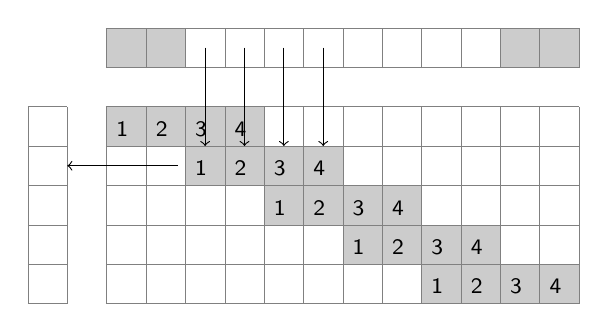
\begin{tikzpicture}[font=\footnotesize\sffamily]
        \fill[black!20!white] (1,3) rectangle (2,3.5);
        \fill[black!20!white] (6,3) rectangle (7,3.5);

        \foreach \x/\y in {0/0, 1/0.5, 2/1, 3/1.5, 4/2}
        {
            \fill[black!20!white] (\x + 1, 2.0 - \y) rectangle (\x + 3, 2.5 - \y);
            \node[above right] at (\x + 1.0, 2 - \y) {1};
            \node[above right] at (\x + 1.5, 2 - \y) {2};
            \node[above right] at (\x + 2.0, 2 - \y) {3};
            \node[above right] at (\x + 2.5, 2 - \y) {4};
        }

        \draw[step=0.5cm,gray,very thin] (0,0) grid (0.5,2.5);
        \draw[step=0.5cm,gray,very thin] (0.99,2.99) grid (7,3.5);
        \draw[step=0.5cm,gray,very thin] (0.99,0) grid (7,2.5);
        \draw [->] (2.25,3.25) -- (2.25,2);
        \draw [->] (2.75,3.25) -- (2.75,2);
        \draw [->] (3.25,3.25) -- (3.25,2);
        \draw [->] (3.75,3.25) -- (3.75,2);
        \draw [->] (1.9,1.75) -- (0.5,1.75);
    \end{tikzpicture}
    \caption{Convolution with stride 2 in 1D \citep{shi_is_2016}}
    \label{fig:1d_deconv}
\end{figure}
For images the output size of a deconvolutional (deconv) layer is calculated with the inverse formula for the output size of a convolutional layer. The stride defines the upsampling factor of this layer, the kernel size the ratio of 'overlapiness' and the padding is set accordingly.

\subsection{Fully convolutional network} % (fold)
\label{sub:conepts:fcn:fcn}
Proposed by \citet{long_fully_2015} \glspl{fcn} are a specific architecture of CNNs. Fully convolutional states that the network consists only of convolutional layers. As these are translation invariant the networks can take arbitrarily sized inputs and produce a coarse output.\\
The original authors use this architecture for semantic segmentation which means to assign each pixel in an image a semantic label (dog, person, tree, etc.). They build their network from classic semantic object classifiers like VGG-16 \citep{simonyan_very_2014}. These take fixed sized images as inputs and produce a single label thereby classifying the whole image. Typically these networks produce high level features through a series of convolutional layers and classify them with a single or a series of fully connected layers (inner product of the inputs). To label an image pixel-wise with such an architecture we would have to forward the neighborhood of each pixel through the network which would introduce an \bigO{w * h} time complexity ($w$ and $h$ being the width and the height of the image).\\
The fully connected layers can be directly converted to convolutional ones.
 These networks (as e.g. ) take full images as input then apply multiple convolutions and in the end classify the whole image with multiple fully connected layers which returns a class prediction vector over the trained classes. Viewing these fully connected layers as convolutions with kernels spanning the whole size of the layers input transforms them in convolutional layers and therefore the whole network into a \gls{fcn}. As the output of this network now will be a small grid of predictions the classification results have to be upsampled to the size of the input which can be done within the network by using deconv layers. Now we have a network which can predict and segment pixelwise in arbitrarily sized inputs and is end-to-end trainable.

\section{Residual Networks}
\label{sec:concepts:resnet}
After the succes of AlexNet \citep{krizhevsky_imagenet_2012}
       % INCLUDE: concepts
% !TEX root = ../thesis.tex
%
\chapter{Pipeline}
\label{sec:pipeline}

\section{Training}
\label{sec:pipeline:training}
\subsection{Preprocessing and augmentation}
\label{sec:pipeline:training:augment}
\begin{figure}[htb]
    \begin{tabularx}{\textwidth}{XXXXX}
        \includegraphics[width=0.170\textwidth]{figures/build/parts_example} &
        \includegraphics[width=0.170\textwidth]{figures/build/parts_example_2} &
        \includegraphics[width=0.170\textwidth]{figures/build/parts_example_18} &
        \includegraphics[width=0.170\textwidth]{figures/build/parts_example_19} &
        \includegraphics[width=0.170\textwidth]{figures/build/parts_example_5} \\

        \includegraphics[width=0.170\textwidth]{figures/build/parts_example_6} &
        \includegraphics[width=0.170\textwidth]{figures/build/parts_example_7} &
        \includegraphics[width=0.170\textwidth]{figures/build/parts_example_8} &
        \includegraphics[width=0.170\textwidth]{figures/build/parts_example_9} &
        \includegraphics[width=0.170\textwidth]{figures/build/parts_example_10}
    \end{tabularx}
	\caption{Top-left is the original patch and the other ones are transformed samples}
    \label{fig:augmentation}
\end{figure}
As we will increasingly reduce the number of samples to train from data augmentation is immensely important. We subtract the mean of all images from the dataset from each training sample \citep{krizhevsky_imagenet_2012}. Moreover we employ multiple image transformations to artificially enlarge the trainings set. For this we use the preprocessing methods provided by the Keras library \citep{chollet_keras:_2015} and add additional transformations. Thus while training we generate new samples online with a set of bounded random transformations. The composite transformation $T_p$ is chosen with the random parameter vector $p = \{\alpha, \beta, s, t_x, t_y, m, t_s, t_v, f_s, f_v, v_s, v_v\}$ defining the following transformations:
\begin{my_list_item}
    \item \textbf{Rotation} with $\alpha\in[-\ang{20}, +\ang{20}]$
    \item \textbf{Shearing} with $\beta\in[-\ang{11.5}, + \ang{11.5}]$
    \item \textbf{Zoom} with $s\in[\SI{70}{\percent}, \SI{130}{\percent}]$
    \item \textbf{Translation} with $t_x,t_y\in[\SI{0}{\percent}, \SI{5}{\percent}]$ of the patches size in either directions on both axes.
    \item \textbf{Flipping} horizontally $m\in\{0,1\}$.
    \item \textbf{Contrast}. Patches are converted to the HSV color space. Saturation and value raised to a power $t_s, t_v \in [0.25, 4]$ then multiplied by factors $f_s, f_v \in [0.7, 1.4]$ and added to some values $v_s, v_v \in [-0.1, 0.1]$ \citep{dosovitskiy_discriminative_2014}. After the contrast transformation patches are again converted to RGB color space.
\end{my_list_item}
We set the parameter boundaries similar to those in \citet{dosovitskiy_discriminative_2014}.

Because the augmentation of training samples severely slows down training if done on demand we generate new samples parallel to the network training.


\section{Generating detections}
\label{sec:pipeline:eval}
Our desired output of the algorithm is one or are multiple boxes enclosing each a section of the image which is predicted to contain the searched for type of object. The \gls{fcn} returns a score map as output. Each score predicts the probability of this pixel to be of the class we trained for. Therefore we need a method to return high scoring bounding boxes from a probability map. The here employed way of doing this consists of multiple steps:\\
\begin{my_list_num}
    \item We penalize (near-) empty regions inside the probability map with a negative distance transform
    \item We generate a set of beforehand defined boxes
    \item For all these boxes we calculate the score density
    \item We apply a low threshold to filter out unnecessary boxes
    \item We apply \gls{nms} to get the top scoring boxes
\end{my_list_num}

\subsection{Negative Distance Transform}
\label{sec:pipeline:eval:dt}
\begin{figure}[htb]
    \begin{tabular}{ccc}
        A probability map & Thresholded map & Distance transform \\[3pt]
        \includegraphics[width=0.303\textwidth]{figures/build/distance_transform_hm-img0} &
        \includegraphics[width=0.303\textwidth]{figures/build/distance_transform_thres-img0} &
        \includegraphics[width=0.303\textwidth]{figures/build/distance_transform_negative-img0}
    \end{tabular}
	\caption{Computing the negative distance transform from an probability map}
    \label{fig:distance_transform}
\end{figure}
A lot of images produce probability maps that are sparsely filled. We want to penalize these regions. Positive regions receive a positive score from the network while not-positive regions are at-most zero. Here we introduce a distance transform to score regions of near-zero values \fref{fig:distance_transform}.\\First we threshold the score map with a near-zero value to set all values that can safely assumed to be negatives to zero.\\Second we apply a distance transform to the zero part of the binary image. A distance transform labels each zero pixel of an image with its distance to the nearest one valued pixel. The distances are valued with some metric like the Euclidean distance or the $L_1$ distance. As the specific metric is not important for our vague penalizer and as we aim for good time performance we use the $L_\infty$ distance also known as the chessboard distance. The transformed image is normalized and substracted from the original probability map.

\subsection{Calculating the score densities}
\label{sec:pipeline:eval:density}
For each forwarded image we generate a set of boxes to calculate the score densities for. At three scales we take boxes of the same aspect ratio as the input image and calculate the slices that would be the result of sliding the window over the image. Also we save the area of all rectangles.\\
Density is calculated by summing up all the probabilities from the score map inside each window and divided by the area of the window. To achieve that as efficiently as possible we use the integral image $I_\Sigma$ of our score map $I$. A value of the integral is the sum of all values left and above this point:
\begin{equation}
    I_\Sigma(x, y) = \sum_{\substack{x' \le x\\ y' \le y}} I(x', y')
\end{equation}
With the integral image the sum inside any rectangle of the image $I$ can then computed efficiently with:
\begin{equation}
    \sum_{\substack{x_0 < x \le x_1\\ y_0 < y \le y_1}}I(x,y) = I_\Sigma(x_1, y_1) + I_\Sigma(x_0, y_0) - I_\Sigma(x_1, y_0) - I_\Sigma(x_0, y_1)
\end{equation}

\subsection{Non maximum suppression}
\label{sec:pipeline:eval:nms}
\begin{figure}[htb]
    \begin{tabular}{ccc}
        Before \gls{nms} & After \gls{nms} \\[3pt]
        \includegraphics[width=0.47\textwidth]{figures/coypu} &
        \includegraphics[width=0.47\textwidth]{figures/coypu}
    \end{tabular}
	\caption{Computing the negative distance transform from an probability map}
    \label{fig:distance_transform}
\end{figure}
Depending on the number of scales we generate hundreds or even thousands of boxes per image. We want to eliminate boxes that are overlapping with another box that has a higher density. Firstly we drop the worst boxes with a low set threshold. While this is not necessary it greatly improves time performance and does not affect testing performance.\\To the remaining boxes we apply \gls{nms} as described by \citet{felzenszwalb_discriminatively_2008}. In the \gls{nms} we first sort all boxes by their descending scores which in our case are the probability densities. We mark the strongest box as picked. Then we calculate the area overlap between the new picked box and all remaining boxes. All boxes with an overlap in area of 0.5 or more are dropped. We pick the next strongest score of the remaining set and continue this process until all boxes are either dropped or picked. The strongest not-overlapping boxes remain picked and are returned. For minimal computational cost of this step we use the improved implementation from \citet{malisiewicz_ensemble_2011}.
         % INCLUDE: system
% !TEX root = ../thesis.tex
%
\chapter{Test results}
\label{sec:results}
Testing of the method is done on the \textsc{Pascal}-Part dataset \citep{Chen_2014_CVPR}, which provides part-based segmentation annotations for images of the \textsc{Pascal}-VOC 2010 challenge dataset \citep{pascal-voc-2010}. For the 20 object classes \textsc{Pascal}-Part contains binary segmentation maps for a selected number of parts of all objects classes.\\
For testing the detection method we train a model with different number of images. From \textsc{Pascal}-Part we pick sets of classes $c \subset C = \{\code{bird, person, train,}\dotsc\}$ and parts $p \subset P = \{\code{head, beak, lhand,}\dotsc\}$. We gather all images from \textsc{Pascal}-VOC 2010 which contain parts $p$ from the classes $c$. Then we extract all patches of these images around the selected parts. We call this set of image patches $I_{c,p}$, e.g. all images of beaks of birds. Then we pick a random subset $I_k$ of $k$ images from $I_{c,p}$ and train the network with this subset. We want to investigate the influence of $k$ on detection results. The remaining set of images $I_{c,p} \setminus I_k$ will be the test set for this single network. For each set $(c,p)$ we take random patches out of the corresponding \textsc{Pascal}-VOC images guaranteeing that they do not overlap with images in $I_{c,p}$. These patches are our negative samples for $(c,p)$ and will be fed into the same data augmentation as the positive samples.

Following in the next chapter we first rationalize our reduced and unequal number of tests \tref{sec:results:repeat}. Next in \treft{sec:results:baseline} we quickly explain the baseline method, which was used as comparison for our results. Finally in \treft{sec:results:results} we report our test results in detection success and time performance \tref{sec:results:time}.

\section{Repeated training and testing}
\label{sec:results:repeat}
Obviously we also have to consider the quality of the subset, not only its size. As we know that a part of the generated and augmented samples is way to small or contains no significant structure to learn, we have to assume that some image patches are not useful for training. Some patches are smaller than $10\times10$ pixels, and others are nearly monochrome. To avoid the influence of bad images, we repeat the training with one set size $k$ multiple times and calculate the mean results of the multiple runs.

Lets assume 30\% of all image patches are useless for training. For how many times do we have to repeat the training with $k$ images, so that we can neglect the influence of these bad samples? To get a rough estimate we reduce this problem to a binary one. First we compute how probable it is that a training will fail for one $k$.\\
The probability $p_b$ that one image is bad is $0.3$. Lets further assume, for simplicity, that a training will still sufficiently succeed if up to $v = 40\%$ of the samples are bad. We get the probability that the training will succeed from the \gls{cdf} of the binomial distribution:
\begin{equation}
    p_s(k) = B_{k,p_b, v k} = \sum_{i=0}^{v k} \binom{k}{i}\cdot p_b^i \cdot (1 - p_b)^{k - i}
\end{equation}
For $k\in\{1, 10, 25, 50, 100\}$ this returns $p_s = \{\num{0.7},\num{0.85},\num{0.902},\num{0.952},\num{0.988}\}$, respectively. These are the probabilities that we will not fail one specific training. The probability that a training fails is $p_f = 1 - p_s = \{\num{0.3},\num{0.15},\num{0.098},\num{0.048},\num{0.012}\}$. Now we want to look at the probability, for an $n$ times repeated run of $k$ images, that half or less of these rounds fail. Again this can be computed with the \gls{cdf}:
\begin{equation}
    p_{repeat}(n,p_f) = B_{n,p_f, \sfrac{n}{2}} = \sum_{i=0}^{\sfrac{n}{2}} \binom{n}{i}\cdot p_f^i \cdot (1 - p_f)^{n - i}
\end{equation}

\begin{table}
	\begin{center}
            \begin{tabular}{c|*{4}{c}}
                samples & 1 round & 2 rounds & 4 rounds & 10 rounds \\ \hline \rule{0pt}{3ex}
                1   & 0.7    &  0.91   &  0.9163 &  0.9527 \\
                10  & 0.8497 &  0.9774 &  0.9880 &  0.9986 \\
                25  & 0.9022 &  0.9904 &  0.9965 &  0.9999  \\
                50  & 0.9522 &  0.9977 &  0.9996 &  0.9999 \\
                100 & 0.9875 &  0.9998 &  0.9999 &  1.
            \end{tabular}
	\end{center}
    \caption{Probabilities that at most half of the rounds fail for different number of samples and different numbers of repetitions.}
    \label{tab:repeated_test_probs}
\end{table}

From the estimations \tabref{tab:repeated_test_probs} we infer that it is sufficient to test the high sampled models way less, than the low sampled ones. Each test, if not noted different, will be the mean results of $\{20, 20, 8, 4, 2\}$ rounds for $\{1, 10, 25, 50, 100\}$ samples, respectively. Through this cascade scheme we reduced the needed test rounds from 100 to only 54, without losing accuracy in test results.

\clearpage
\section{Baseline}
\label{sec:results:baseline}
To compare our results we additionally solve the task with a baseline method. We build a simple object detector inspired by \citet{felzenszwalb_object_2010} using \acrfull{hog} \citep{dalal_histograms_2005}.\\

\subsection{\Gls{hog}}
\begin{wrapfigure}{r}{0.45\textwidth}
  \vspace{-25pt}
  \begin{center}
    \includegraphics[width=0.17\textwidth]{figures/hog_image.png}
    \includegraphics[width=0.17\textwidth]{figures/hog_feature.png}
  \end{center}
  \vspace{-5pt}
  \caption{A example of a patch and  the resulting \gls{hog} cells.}
  \vspace{-10pt}
  \label{fig:hog}
\end{wrapfigure}
\gls{hog} features encode the shape of an object assuming that its shape can be described by the distribution of edge directions. As the name already states we want to look at the gradients of the image at different orientations. We compute the horizontal and vertical gradients from the relative luminance of the original image, using the standard weighted channel contributions. To get the spatial localization we split the image into small regions called cells. For each cell we compute the histogram, which is just an $1d$ vector containing the gradients over a fixed set of angles in that cell. Next we group these cells into larger overlapping blocks. The blocks are used to normalize the contained histograms. This introduces better invariance to illumination and edge contrast. As the blocks are overlapping, each cell will appear multiple times in the output but under different normalization. For normalization we use the L2-norm followed by clipping \citep{lowe_distinctive_2004}.

\subsection{Training}
We collect $1000$ samples of augmented samples, using the same method as described in \treft{sec:pipeline:training:augment}. For all samples we compute the \gls{hog} features using the settings as in \citep{dalal_histograms_2005}. In \citet{felzenszwalb_object_2010} their model consists of multiple parts each described by its own \gls{hog} features. Because we will only train for small parts we describe each sample by only one \gls{hog} descriptor at one scale. Using the set of balanced positive and negative samples we train a linear \gls{svm}.
\clearpage
\subsection{Testing}
The testing pipeline should be as similar as possible to the novel method. To use the same box generation, density calculation and \gls{nms} as in \treft{sec:pipeline:eval}, we need a map of class probability predictions as input. Sliding a window over the images and computing the \gls{hog} features for all positions in the image is rather inefficient. Instead we compute the \gls{hog} descriptors for the whole image and classify a window that is slided over the feature map. The \gls{svm} returns the predicted class (background \textit{vs} foreground), and the scores are aggregated for all windows to build the needed probability map. Although it is not useful to train a multi-scale classifier for our small training samples, we have to take differently scaled test objects into account. Thus we test on multiple scales. Because the \gls{svm} needs a fixed shape, the same number of \gls{hog} blocks, as input to predict their class, we change the \gls{hog} parameters for the different scales. For windows half the size we also halve the width of each \gls{hog} cell, thus resulting in the same number of blocks per window.

\clearpage
\section{Detection results}
\label{sec:results:results}
\begin{figure}[htb]
    \setlength\tabcolsep{0pt}
    \renewcommand{\arraystretch}{0}
    \begin{tabular}{ccccccc}
      \includegraphics[height=1.8cm]{figures/hm_examples/1s_2008_002067} &
      \includegraphics[height=1.8cm]{figures/hm_examples/1s_2009_004323} &
      \includegraphics[height=1.8cm]{figures/hm_examples/1s_2009_004784} &
      \includegraphics[height=1.8cm]{figures/hm_examples/1s_2009_005222} &
      \includegraphics[height=1.8cm]{figures/hm_examples/1s_2009_002715} &
      \includegraphics[height=1.8cm]{figures/hm_examples/1s_2010_005967} \\
      \includegraphics[height=1.8cm]{figures/hm_examples/1s_bbox_2008_002067} &
      \includegraphics[height=1.8cm]{figures/hm_examples/1s_bbox_2009_004323} &
      \includegraphics[height=1.8cm]{figures/hm_examples/1s_bbox_2009_004784} &
      \includegraphics[height=1.8cm]{figures/hm_examples/1s_bbox_2009_005222} &
      \includegraphics[height=1.8cm]{figures/hm_examples/1s_bbox_2009_002715} &
      \includegraphics[height=1.8cm]{figures/hm_examples/1s_bbox_2010_005967} \\[3pt]

      \includegraphics[height=1.8cm]{figures/hm_examples/50s_2008_002067} &
      \includegraphics[height=1.8cm]{figures/hm_examples/50s_2009_004323} &
      \includegraphics[height=1.8cm]{figures/hm_examples/50s_2009_004784} &
      \includegraphics[height=1.8cm]{figures/hm_examples/50s_2009_005222} &
      \includegraphics[height=1.8cm]{figures/hm_examples/50s_2009_002715} &
      \includegraphics[height=1.8cm]{figures/hm_examples/50s_2010_005967} \\
      \includegraphics[height=1.8cm]{figures/hm_examples/50s_bbox_2008_002067} &
      \includegraphics[height=1.8cm]{figures/hm_examples/50s_bbox_2009_004323} &
      \includegraphics[height=1.8cm]{figures/hm_examples/50s_bbox_2009_004784} &
      \includegraphics[height=1.8cm]{figures/hm_examples/50s_bbox_2009_005222} &
      \includegraphics[height=1.8cm]{figures/hm_examples/50s_bbox_2009_002715} &
      \includegraphics[height=1.8cm]{figures/hm_examples/50s_bbox_2010_005967}

    \end{tabular}
	\caption{Examples from \code{person\_hair}: Top detections are from a run with 1 sample, bottom detections are from a run with 50 samples. Note how the 50 sampled network detects more variations of the parts while the other one does not. Also note how both networks miss-detect the cats head as human hair.}
  \label{fig:hm_examples}
\end{figure}
We test the pipeline for the class-parts combinations $(c,p)$ listed in appendix \ref{sec:appendix:combos}, using the cascade scheme described in \treft{sec:results:repeat}. To evaluate the detection we collect all predicted bounding boxes for all images and their scores.

For a summary of test results see \figreft{fig:auc_heatmap}. We clearly see the correlation between set size and the success in testing. Training with only one sample returns the worst results, by distance, with a mean \gls{auc} over all parts and all runs of 0.72. With increasing set size the test results saturate quickly. The mean \gls{auc} for all larger set sizes lie inside a range of only 0.03. That may be explainable with our training settings, which are designed for fast training and has no time to incorporate a high number of examples into the representation learning.\TODO{add baseline comparsion}

Besides the anticipated correlation between set size and test success, we also show the correlation between different object parts and the success in quickly learning their representation. An example for this difference is given in \figreft{fig:pr_example}. Training on human hair was one of the more successful experiments while training on human necks does not return a useful classifier. The difference can be explained by the amount of discriminating structure a part has to offer. While necks most of the time are very small mostly contrast-less and structure-less patches, hair has a distinguishable surface and therefore more recognizable visual features.

\begin{figure}
  \begin{tabular}{cc}
    \prplot{person_hair} &
    \prplot{person_neck}
  \end{tabular}
  \caption{Precision-Recall curves for two parts. \code{person\_hair} on the left as an successful example and \code{person\_neck} as an example for an utterly failed training. Certainly though we see in both plots the clear separation between different set sizes.}
  \label{fig:pr_example}
\end{figure}

Another potential explanation stems from our training method. We train our classifier not on the pixel-precise masks, that \textsc{Pascal}-Part provide, but on rectangular patches retrieved from the original images around each part. As such a patch of human hair will, most of the time, contain a section of the head underneath. One therefore can expect that the model not only learns the representation of the part itself but also of the surrounding object segments. We see this relation in the quite similar results of \code{person\_hair} and \code{person\_head}. Firstly such spatial relations are only relevant in some cases, and secondly while this may frustrate part-based training in some cases, most of the time spatial relations to semantically related parts are an actual indicator for the searched part. If we search for human hair and find human heads, we also found many instances of human hair.

Furthermore we want to check that the cascade testing scheme was intensive enough to report sufficiently precise results. We calculate the variance of \gls{auc} scores for the different parts and training sizes to verify their precision \fref{fig:auc_var_heatmap}. As we expected the variance drastically decreases with increasing set size, and as such we conclude our testing scheme to be adequate for this random sampling. Even for the 20 times repeated 1 sampled training runs, the variance of \gls{auc} scores remains under 0.02 most of the times.
\begin{figure}[p!h]
    \centering
    %% Creator: Matplotlib, PGF backend
%%
%% To include the figure in your LaTeX document, write
%%   \input{<filename>.pgf}
%%
%% Make sure the required packages are loaded in your preamble
%%   \usepackage{pgf}
%%
%% Figures using additional raster images can only be included by \input if
%% they are in the same directory as the main LaTeX file. For loading figures
%% from other directories you can use the `import` package
%%   \usepackage{import}
%% and then include the figures with
%%   \import{<path to file>}{<filename>.pgf}
%%
%% Matplotlib used the following preamble
%%   \usepackage[utf8x]{inputenc}
%%   \usepackage[T1]{fontenc}
%%
\begingroup%
\makeatletter%
\begin{pgfpicture}%
\pgfpathrectangle{\pgfpointorigin}{\pgfqpoint{5.307713in}{6.232660in}}%
\pgfusepath{use as bounding box, clip}%
\begin{pgfscope}%
\pgfsetbuttcap%
\pgfsetmiterjoin%
\definecolor{currentfill}{rgb}{1.000000,1.000000,1.000000}%
\pgfsetfillcolor{currentfill}%
\pgfsetlinewidth{0.000000pt}%
\definecolor{currentstroke}{rgb}{1.000000,1.000000,1.000000}%
\pgfsetstrokecolor{currentstroke}%
\pgfsetdash{}{0pt}%
\pgfpathmoveto{\pgfqpoint{0.000000in}{0.000000in}}%
\pgfpathlineto{\pgfqpoint{5.307713in}{0.000000in}}%
\pgfpathlineto{\pgfqpoint{5.307713in}{6.232660in}}%
\pgfpathlineto{\pgfqpoint{0.000000in}{6.232660in}}%
\pgfpathclose%
\pgfusepath{fill}%
\end{pgfscope}%
\begin{pgfscope}%
\pgfsetbuttcap%
\pgfsetmiterjoin%
\definecolor{currentfill}{rgb}{1.000000,1.000000,1.000000}%
\pgfsetfillcolor{currentfill}%
\pgfsetlinewidth{0.000000pt}%
\definecolor{currentstroke}{rgb}{0.000000,0.000000,0.000000}%
\pgfsetstrokecolor{currentstroke}%
\pgfsetstrokeopacity{0.000000}%
\pgfsetdash{}{0pt}%
\pgfpathmoveto{\pgfqpoint{1.535693in}{0.322448in}}%
\pgfpathlineto{\pgfqpoint{5.163713in}{0.322448in}}%
\pgfpathlineto{\pgfqpoint{5.163713in}{6.088660in}}%
\pgfpathlineto{\pgfqpoint{1.535693in}{6.088660in}}%
\pgfpathclose%
\pgfusepath{fill}%
\end{pgfscope}%
\begin{pgfscope}%
\definecolor{textcolor}{rgb}{0.150000,0.150000,0.150000}%
\pgfsetstrokecolor{textcolor}%
\pgfsetfillcolor{textcolor}%
\pgftext[x=1.898495in,y=0.244670in,,top]{\color{textcolor}\sffamily\fontsize{8.000000}{9.600000}\selectfont 1}%
\end{pgfscope}%
\begin{pgfscope}%
\definecolor{textcolor}{rgb}{0.150000,0.150000,0.150000}%
\pgfsetstrokecolor{textcolor}%
\pgfsetfillcolor{textcolor}%
\pgftext[x=2.624099in,y=0.244670in,,top]{\color{textcolor}\sffamily\fontsize{8.000000}{9.600000}\selectfont 10}%
\end{pgfscope}%
\begin{pgfscope}%
\definecolor{textcolor}{rgb}{0.150000,0.150000,0.150000}%
\pgfsetstrokecolor{textcolor}%
\pgfsetfillcolor{textcolor}%
\pgftext[x=3.349703in,y=0.244670in,,top]{\color{textcolor}\sffamily\fontsize{8.000000}{9.600000}\selectfont 25}%
\end{pgfscope}%
\begin{pgfscope}%
\definecolor{textcolor}{rgb}{0.150000,0.150000,0.150000}%
\pgfsetstrokecolor{textcolor}%
\pgfsetfillcolor{textcolor}%
\pgftext[x=4.075307in,y=0.244670in,,top]{\color{textcolor}\sffamily\fontsize{8.000000}{9.600000}\selectfont 50}%
\end{pgfscope}%
\begin{pgfscope}%
\definecolor{textcolor}{rgb}{0.150000,0.150000,0.150000}%
\pgfsetstrokecolor{textcolor}%
\pgfsetfillcolor{textcolor}%
\pgftext[x=4.800911in,y=0.244670in,,top]{\color{textcolor}\sffamily\fontsize{8.000000}{9.600000}\selectfont 100}%
\end{pgfscope}%
\begin{pgfscope}%
\definecolor{textcolor}{rgb}{0.150000,0.150000,0.150000}%
\pgfsetstrokecolor{textcolor}%
\pgfsetfillcolor{textcolor}%
\pgftext[x=1.184834in,y=0.403042in,left,base]{\color{textcolor}\sffamily\fontsize{8.000000}{9.600000}\selectfont Mean}%
\end{pgfscope}%
\begin{pgfscope}%
\definecolor{textcolor}{rgb}{0.150000,0.150000,0.150000}%
\pgfsetstrokecolor{textcolor}%
\pgfsetfillcolor{textcolor}%
\pgftext[x=0.650705in,y=0.643301in,left,base]{\color{textcolor}\sffamily\fontsize{8.000000}{9.600000}\selectfont train\_hfrontside}%
\end{pgfscope}%
\begin{pgfscope}%
\definecolor{textcolor}{rgb}{0.150000,0.150000,0.150000}%
\pgfsetstrokecolor{textcolor}%
\pgfsetfillcolor{textcolor}%
\pgftext[x=0.906353in,y=0.883560in,left,base]{\color{textcolor}\sffamily\fontsize{8.000000}{9.600000}\selectfont train\_head}%
\end{pgfscope}%
\begin{pgfscope}%
\definecolor{textcolor}{rgb}{0.150000,0.150000,0.150000}%
\pgfsetstrokecolor{textcolor}%
\pgfsetfillcolor{textcolor}%
\pgftext[x=0.855825in,y=1.123818in,left,base]{\color{textcolor}\sffamily\fontsize{8.000000}{9.600000}\selectfont train\_coach}%
\end{pgfscope}%
\begin{pgfscope}%
\definecolor{textcolor}{rgb}{0.150000,0.150000,0.150000}%
\pgfsetstrokecolor{textcolor}%
\pgfsetfillcolor{textcolor}%
\pgftext[x=0.545522in,y=1.364077in,left,base]{\color{textcolor}\sffamily\fontsize{8.000000}{9.600000}\selectfont pottedplant\_plant}%
\end{pgfscope}%
\begin{pgfscope}%
\definecolor{textcolor}{rgb}{0.150000,0.150000,0.150000}%
\pgfsetstrokecolor{textcolor}%
\pgfsetfillcolor{textcolor}%
\pgftext[x=0.801016in,y=1.609659in,left,base]{\color{textcolor}\sffamily\fontsize{8.000000}{9.600000}\selectfont person\_torso}%
\end{pgfscope}%
\begin{pgfscope}%
\definecolor{textcolor}{rgb}{0.150000,0.150000,0.150000}%
\pgfsetstrokecolor{textcolor}%
\pgfsetfillcolor{textcolor}%
\pgftext[x=0.820417in,y=1.844595in,left,base]{\color{textcolor}\sffamily\fontsize{8.000000}{9.600000}\selectfont person\_neck}%
\end{pgfscope}%
\begin{pgfscope}%
\definecolor{textcolor}{rgb}{0.150000,0.150000,0.150000}%
\pgfsetstrokecolor{textcolor}%
\pgfsetfillcolor{textcolor}%
\pgftext[x=0.404623in,y=2.084854in,left,base]{\color{textcolor}\sffamily\fontsize{8.000000}{9.600000}\selectfont person\_lhand\_rhand}%
\end{pgfscope}%
\begin{pgfscope}%
\definecolor{textcolor}{rgb}{0.150000,0.150000,0.150000}%
\pgfsetstrokecolor{textcolor}%
\pgfsetfillcolor{textcolor}%
\pgftext[x=0.483693in,y=2.325113in,left,base]{\color{textcolor}\sffamily\fontsize{8.000000}{9.600000}\selectfont person\_lfoot\_rfoot}%
\end{pgfscope}%
\begin{pgfscope}%
\definecolor{textcolor}{rgb}{0.150000,0.150000,0.150000}%
\pgfsetstrokecolor{textcolor}%
\pgfsetfillcolor{textcolor}%
\pgftext[x=0.591306in,y=2.565372in,left,base]{\color{textcolor}\sffamily\fontsize{8.000000}{9.600000}\selectfont person\_lear\_rear}%
\end{pgfscope}%
\begin{pgfscope}%
\definecolor{textcolor}{rgb}{0.150000,0.150000,0.150000}%
\pgfsetstrokecolor{textcolor}%
\pgfsetfillcolor{textcolor}%
\pgftext[x=0.812895in,y=2.805630in,left,base]{\color{textcolor}\sffamily\fontsize{8.000000}{9.600000}\selectfont person\_head}%
\end{pgfscope}%
\begin{pgfscope}%
\definecolor{textcolor}{rgb}{0.150000,0.150000,0.150000}%
\pgfsetstrokecolor{textcolor}%
\pgfsetfillcolor{textcolor}%
\pgftext[x=0.857830in,y=3.045889in,left,base]{\color{textcolor}\sffamily\fontsize{8.000000}{9.600000}\selectfont person\_hair}%
\end{pgfscope}%
\begin{pgfscope}%
\definecolor{textcolor}{rgb}{0.150000,0.150000,0.150000}%
\pgfsetstrokecolor{textcolor}%
\pgfsetfillcolor{textcolor}%
\pgftext[x=0.144000in,y=3.286148in,left,base]{\color{textcolor}\sffamily\fontsize{8.000000}{9.600000}\selectfont motorbike\_bwheel\_fwheel}%
\end{pgfscope}%
\begin{pgfscope}%
\definecolor{textcolor}{rgb}{0.150000,0.150000,0.150000}%
\pgfsetstrokecolor{textcolor}%
\pgfsetfillcolor{textcolor}%
\pgftext[x=0.217362in,y=3.526407in,left,base]{\color{textcolor}\sffamily\fontsize{8.000000}{9.600000}\selectfont cow\_sheep\_lhorn\_rhorn}%
\end{pgfscope}%
\begin{pgfscope}%
\definecolor{textcolor}{rgb}{0.150000,0.150000,0.150000}%
\pgfsetstrokecolor{textcolor}%
\pgfsetfillcolor{textcolor}%
\pgftext[x=1.000658in,y=3.766666in,left,base]{\color{textcolor}\sffamily\fontsize{8.000000}{9.600000}\selectfont car\_door}%
\end{pgfscope}%
\begin{pgfscope}%
\definecolor{textcolor}{rgb}{0.150000,0.150000,0.150000}%
\pgfsetstrokecolor{textcolor}%
\pgfsetfillcolor{textcolor}%
\pgftext[x=0.178791in,y=4.006925in,left,base]{\color{textcolor}\sffamily\fontsize{8.000000}{9.600000}\selectfont bus\_car\_bliplate\_fliplate}%
\end{pgfscope}%
\begin{pgfscope}%
\definecolor{textcolor}{rgb}{0.150000,0.150000,0.150000}%
\pgfsetstrokecolor{textcolor}%
\pgfsetfillcolor{textcolor}%
\pgftext[x=0.835189in,y=4.247183in,left,base]{\color{textcolor}\sffamily\fontsize{8.000000}{9.600000}\selectfont bottle\_body}%
\end{pgfscope}%
\begin{pgfscope}%
\definecolor{textcolor}{rgb}{0.150000,0.150000,0.150000}%
\pgfsetstrokecolor{textcolor}%
\pgfsetfillcolor{textcolor}%
\pgftext[x=1.020136in,y=4.487442in,left,base]{\color{textcolor}\sffamily\fontsize{8.000000}{9.600000}\selectfont bird\_tail}%
\end{pgfscope}%
\begin{pgfscope}%
\definecolor{textcolor}{rgb}{0.150000,0.150000,0.150000}%
\pgfsetstrokecolor{textcolor}%
\pgfsetfillcolor{textcolor}%
\pgftext[x=0.558058in,y=4.727701in,left,base]{\color{textcolor}\sffamily\fontsize{8.000000}{9.600000}\selectfont bird\_lwing\_rwing}%
\end{pgfscope}%
\begin{pgfscope}%
\definecolor{textcolor}{rgb}{0.150000,0.150000,0.150000}%
\pgfsetstrokecolor{textcolor}%
\pgfsetfillcolor{textcolor}%
\pgftext[x=0.944730in,y=4.967960in,left,base]{\color{textcolor}\sffamily\fontsize{8.000000}{9.600000}\selectfont bird\_head}%
\end{pgfscope}%
\begin{pgfscope}%
\definecolor{textcolor}{rgb}{0.150000,0.150000,0.150000}%
\pgfsetstrokecolor{textcolor}%
\pgfsetfillcolor{textcolor}%
\pgftext[x=0.944730in,y=5.208219in,left,base]{\color{textcolor}\sffamily\fontsize{8.000000}{9.600000}\selectfont bird\_beak}%
\end{pgfscope}%
\begin{pgfscope}%
\definecolor{textcolor}{rgb}{0.150000,0.150000,0.150000}%
\pgfsetstrokecolor{textcolor}%
\pgfsetfillcolor{textcolor}%
\pgftext[x=0.302333in,y=5.448478in,left,base]{\color{textcolor}\sffamily\fontsize{8.000000}{9.600000}\selectfont bicycle\_bwheel\_fwheel}%
\end{pgfscope}%
\begin{pgfscope}%
\definecolor{textcolor}{rgb}{0.150000,0.150000,0.150000}%
\pgfsetstrokecolor{textcolor}%
\pgfsetfillcolor{textcolor}%
\pgftext[x=0.656876in,y=5.688736in,left,base]{\color{textcolor}\sffamily\fontsize{8.000000}{9.600000}\selectfont aeroplane\_stern}%
\end{pgfscope}%
\begin{pgfscope}%
\definecolor{textcolor}{rgb}{0.150000,0.150000,0.150000}%
\pgfsetstrokecolor{textcolor}%
\pgfsetfillcolor{textcolor}%
\pgftext[x=0.280734in,y=5.928995in,left,base]{\color{textcolor}\sffamily\fontsize{8.000000}{9.600000}\selectfont aeroplane\_lwing\_rwing}%
\end{pgfscope}%
\begin{pgfscope}%
\pgfpathrectangle{\pgfqpoint{1.535693in}{0.322448in}}{\pgfqpoint{3.628020in}{5.766212in}} %
\pgfusepath{clip}%
\pgfsetbuttcap%
\pgfsetroundjoin%
\definecolor{currentfill}{rgb}{0.590934,0.737671,0.527775}%
\pgfsetfillcolor{currentfill}%
\pgfsetlinewidth{0.000000pt}%
\definecolor{currentstroke}{rgb}{1.000000,1.000000,1.000000}%
\pgfsetstrokecolor{currentstroke}%
\pgfsetdash{}{0pt}%
\pgfpathmoveto{\pgfqpoint{1.535693in}{0.322448in}}%
\pgfpathlineto{\pgfqpoint{2.261297in}{0.322448in}}%
\pgfpathlineto{\pgfqpoint{2.261297in}{0.562706in}}%
\pgfpathlineto{\pgfqpoint{1.535693in}{0.562706in}}%
\pgfpathlineto{\pgfqpoint{1.535693in}{0.322448in}}%
\pgfusepath{fill}%
\end{pgfscope}%
\begin{pgfscope}%
\pgfpathrectangle{\pgfqpoint{1.535693in}{0.322448in}}{\pgfqpoint{3.628020in}{5.766212in}} %
\pgfusepath{clip}%
\pgfsetbuttcap%
\pgfsetroundjoin%
\definecolor{currentfill}{rgb}{0.412288,0.617543,0.397417}%
\pgfsetfillcolor{currentfill}%
\pgfsetlinewidth{0.000000pt}%
\definecolor{currentstroke}{rgb}{1.000000,1.000000,1.000000}%
\pgfsetstrokecolor{currentstroke}%
\pgfsetdash{}{0pt}%
\pgfpathmoveto{\pgfqpoint{2.261297in}{0.322448in}}%
\pgfpathlineto{\pgfqpoint{2.986901in}{0.322448in}}%
\pgfpathlineto{\pgfqpoint{2.986901in}{0.562706in}}%
\pgfpathlineto{\pgfqpoint{2.261297in}{0.562706in}}%
\pgfpathlineto{\pgfqpoint{2.261297in}{0.322448in}}%
\pgfusepath{fill}%
\end{pgfscope}%
\begin{pgfscope}%
\pgfpathrectangle{\pgfqpoint{1.535693in}{0.322448in}}{\pgfqpoint{3.628020in}{5.766212in}} %
\pgfusepath{clip}%
\pgfsetbuttcap%
\pgfsetroundjoin%
\definecolor{currentfill}{rgb}{0.390531,0.600670,0.382428}%
\pgfsetfillcolor{currentfill}%
\pgfsetlinewidth{0.000000pt}%
\definecolor{currentstroke}{rgb}{1.000000,1.000000,1.000000}%
\pgfsetstrokecolor{currentstroke}%
\pgfsetdash{}{0pt}%
\pgfpathmoveto{\pgfqpoint{2.986901in}{0.322448in}}%
\pgfpathlineto{\pgfqpoint{3.712505in}{0.322448in}}%
\pgfpathlineto{\pgfqpoint{3.712505in}{0.562706in}}%
\pgfpathlineto{\pgfqpoint{2.986901in}{0.562706in}}%
\pgfpathlineto{\pgfqpoint{2.986901in}{0.322448in}}%
\pgfusepath{fill}%
\end{pgfscope}%
\begin{pgfscope}%
\pgfpathrectangle{\pgfqpoint{1.535693in}{0.322448in}}{\pgfqpoint{3.628020in}{5.766212in}} %
\pgfusepath{clip}%
\pgfsetbuttcap%
\pgfsetroundjoin%
\definecolor{currentfill}{rgb}{0.381813,0.593723,0.376436}%
\pgfsetfillcolor{currentfill}%
\pgfsetlinewidth{0.000000pt}%
\definecolor{currentstroke}{rgb}{1.000000,1.000000,1.000000}%
\pgfsetstrokecolor{currentstroke}%
\pgfsetdash{}{0pt}%
\pgfpathmoveto{\pgfqpoint{3.712505in}{0.322448in}}%
\pgfpathlineto{\pgfqpoint{4.438109in}{0.322448in}}%
\pgfpathlineto{\pgfqpoint{4.438109in}{0.562706in}}%
\pgfpathlineto{\pgfqpoint{3.712505in}{0.562706in}}%
\pgfpathlineto{\pgfqpoint{3.712505in}{0.322448in}}%
\pgfusepath{fill}%
\end{pgfscope}%
\begin{pgfscope}%
\pgfpathrectangle{\pgfqpoint{1.535693in}{0.322448in}}{\pgfqpoint{3.628020in}{5.766212in}} %
\pgfusepath{clip}%
\pgfsetbuttcap%
\pgfsetroundjoin%
\definecolor{currentfill}{rgb}{0.377452,0.590206,0.373439}%
\pgfsetfillcolor{currentfill}%
\pgfsetlinewidth{0.000000pt}%
\definecolor{currentstroke}{rgb}{1.000000,1.000000,1.000000}%
\pgfsetstrokecolor{currentstroke}%
\pgfsetdash{}{0pt}%
\pgfpathmoveto{\pgfqpoint{4.438109in}{0.322448in}}%
\pgfpathlineto{\pgfqpoint{5.163713in}{0.322448in}}%
\pgfpathlineto{\pgfqpoint{5.163713in}{0.562706in}}%
\pgfpathlineto{\pgfqpoint{4.438109in}{0.562706in}}%
\pgfpathlineto{\pgfqpoint{4.438109in}{0.322448in}}%
\pgfusepath{fill}%
\end{pgfscope}%
\begin{pgfscope}%
\pgfpathrectangle{\pgfqpoint{1.535693in}{0.322448in}}{\pgfqpoint{3.628020in}{5.766212in}} %
\pgfusepath{clip}%
\pgfsetbuttcap%
\pgfsetroundjoin%
\definecolor{currentfill}{rgb}{0.515548,0.690222,0.470524}%
\pgfsetfillcolor{currentfill}%
\pgfsetlinewidth{0.000000pt}%
\definecolor{currentstroke}{rgb}{1.000000,1.000000,1.000000}%
\pgfsetstrokecolor{currentstroke}%
\pgfsetdash{}{0pt}%
\pgfpathmoveto{\pgfqpoint{1.535693in}{0.562706in}}%
\pgfpathlineto{\pgfqpoint{2.261297in}{0.562706in}}%
\pgfpathlineto{\pgfqpoint{2.261297in}{0.802965in}}%
\pgfpathlineto{\pgfqpoint{1.535693in}{0.802965in}}%
\pgfpathlineto{\pgfqpoint{1.535693in}{0.562706in}}%
\pgfusepath{fill}%
\end{pgfscope}%
\begin{pgfscope}%
\pgfpathrectangle{\pgfqpoint{1.535693in}{0.322448in}}{\pgfqpoint{3.628020in}{5.766212in}} %
\pgfusepath{clip}%
\pgfsetbuttcap%
\pgfsetroundjoin%
\definecolor{currentfill}{rgb}{0.346883,0.564708,0.352416}%
\pgfsetfillcolor{currentfill}%
\pgfsetlinewidth{0.000000pt}%
\definecolor{currentstroke}{rgb}{1.000000,1.000000,1.000000}%
\pgfsetstrokecolor{currentstroke}%
\pgfsetdash{}{0pt}%
\pgfpathmoveto{\pgfqpoint{2.261297in}{0.562706in}}%
\pgfpathlineto{\pgfqpoint{2.986901in}{0.562706in}}%
\pgfpathlineto{\pgfqpoint{2.986901in}{0.802965in}}%
\pgfpathlineto{\pgfqpoint{2.261297in}{0.802965in}}%
\pgfpathlineto{\pgfqpoint{2.261297in}{0.562706in}}%
\pgfusepath{fill}%
\end{pgfscope}%
\begin{pgfscope}%
\pgfpathrectangle{\pgfqpoint{1.535693in}{0.322448in}}{\pgfqpoint{3.628020in}{5.766212in}} %
\pgfusepath{clip}%
\pgfsetbuttcap%
\pgfsetroundjoin%
\definecolor{currentfill}{rgb}{0.342512,0.560933,0.349402}%
\pgfsetfillcolor{currentfill}%
\pgfsetlinewidth{0.000000pt}%
\definecolor{currentstroke}{rgb}{1.000000,1.000000,1.000000}%
\pgfsetstrokecolor{currentstroke}%
\pgfsetdash{}{0pt}%
\pgfpathmoveto{\pgfqpoint{2.986901in}{0.562706in}}%
\pgfpathlineto{\pgfqpoint{3.712505in}{0.562706in}}%
\pgfpathlineto{\pgfqpoint{3.712505in}{0.802965in}}%
\pgfpathlineto{\pgfqpoint{2.986901in}{0.802965in}}%
\pgfpathlineto{\pgfqpoint{2.986901in}{0.562706in}}%
\pgfusepath{fill}%
\end{pgfscope}%
\begin{pgfscope}%
\pgfpathrectangle{\pgfqpoint{1.535693in}{0.322448in}}{\pgfqpoint{3.628020in}{5.766212in}} %
\pgfusepath{clip}%
\pgfsetbuttcap%
\pgfsetroundjoin%
\definecolor{currentfill}{rgb}{0.359992,0.575829,0.361440}%
\pgfsetfillcolor{currentfill}%
\pgfsetlinewidth{0.000000pt}%
\definecolor{currentstroke}{rgb}{1.000000,1.000000,1.000000}%
\pgfsetstrokecolor{currentstroke}%
\pgfsetdash{}{0pt}%
\pgfpathmoveto{\pgfqpoint{3.712505in}{0.562706in}}%
\pgfpathlineto{\pgfqpoint{4.438109in}{0.562706in}}%
\pgfpathlineto{\pgfqpoint{4.438109in}{0.802965in}}%
\pgfpathlineto{\pgfqpoint{3.712505in}{0.802965in}}%
\pgfpathlineto{\pgfqpoint{3.712505in}{0.562706in}}%
\pgfusepath{fill}%
\end{pgfscope}%
\begin{pgfscope}%
\pgfpathrectangle{\pgfqpoint{1.535693in}{0.322448in}}{\pgfqpoint{3.628020in}{5.766212in}} %
\pgfusepath{clip}%
\pgfsetbuttcap%
\pgfsetroundjoin%
\definecolor{currentfill}{rgb}{0.359992,0.575829,0.361440}%
\pgfsetfillcolor{currentfill}%
\pgfsetlinewidth{0.000000pt}%
\definecolor{currentstroke}{rgb}{1.000000,1.000000,1.000000}%
\pgfsetstrokecolor{currentstroke}%
\pgfsetdash{}{0pt}%
\pgfpathmoveto{\pgfqpoint{4.438109in}{0.562706in}}%
\pgfpathlineto{\pgfqpoint{5.163713in}{0.562706in}}%
\pgfpathlineto{\pgfqpoint{5.163713in}{0.802965in}}%
\pgfpathlineto{\pgfqpoint{4.438109in}{0.802965in}}%
\pgfpathlineto{\pgfqpoint{4.438109in}{0.562706in}}%
\pgfusepath{fill}%
\end{pgfscope}%
\begin{pgfscope}%
\pgfpathrectangle{\pgfqpoint{1.535693in}{0.322448in}}{\pgfqpoint{3.628020in}{5.766212in}} %
\pgfusepath{clip}%
\pgfsetbuttcap%
\pgfsetroundjoin%
\definecolor{currentfill}{rgb}{0.285645,0.508428,0.309642}%
\pgfsetfillcolor{currentfill}%
\pgfsetlinewidth{0.000000pt}%
\definecolor{currentstroke}{rgb}{1.000000,1.000000,1.000000}%
\pgfsetstrokecolor{currentstroke}%
\pgfsetdash{}{0pt}%
\pgfpathmoveto{\pgfqpoint{1.535693in}{0.802965in}}%
\pgfpathlineto{\pgfqpoint{2.261297in}{0.802965in}}%
\pgfpathlineto{\pgfqpoint{2.261297in}{1.043224in}}%
\pgfpathlineto{\pgfqpoint{1.535693in}{1.043224in}}%
\pgfpathlineto{\pgfqpoint{1.535693in}{0.802965in}}%
\pgfusepath{fill}%
\end{pgfscope}%
\begin{pgfscope}%
\pgfpathrectangle{\pgfqpoint{1.535693in}{0.322448in}}{\pgfqpoint{3.628020in}{5.766212in}} %
\pgfusepath{clip}%
\pgfsetbuttcap%
\pgfsetroundjoin%
\definecolor{currentfill}{rgb}{0.298770,0.521154,0.318941}%
\pgfsetfillcolor{currentfill}%
\pgfsetlinewidth{0.000000pt}%
\definecolor{currentstroke}{rgb}{1.000000,1.000000,1.000000}%
\pgfsetstrokecolor{currentstroke}%
\pgfsetdash{}{0pt}%
\pgfpathmoveto{\pgfqpoint{2.261297in}{0.802965in}}%
\pgfpathlineto{\pgfqpoint{2.986901in}{0.802965in}}%
\pgfpathlineto{\pgfqpoint{2.986901in}{1.043224in}}%
\pgfpathlineto{\pgfqpoint{2.261297in}{1.043224in}}%
\pgfpathlineto{\pgfqpoint{2.261297in}{0.802965in}}%
\pgfusepath{fill}%
\end{pgfscope}%
\begin{pgfscope}%
\pgfpathrectangle{\pgfqpoint{1.535693in}{0.322448in}}{\pgfqpoint{3.628020in}{5.766212in}} %
\pgfusepath{clip}%
\pgfsetbuttcap%
\pgfsetroundjoin%
\definecolor{currentfill}{rgb}{0.303146,0.525309,0.322021}%
\pgfsetfillcolor{currentfill}%
\pgfsetlinewidth{0.000000pt}%
\definecolor{currentstroke}{rgb}{1.000000,1.000000,1.000000}%
\pgfsetstrokecolor{currentstroke}%
\pgfsetdash{}{0pt}%
\pgfpathmoveto{\pgfqpoint{2.986901in}{0.802965in}}%
\pgfpathlineto{\pgfqpoint{3.712505in}{0.802965in}}%
\pgfpathlineto{\pgfqpoint{3.712505in}{1.043224in}}%
\pgfpathlineto{\pgfqpoint{2.986901in}{1.043224in}}%
\pgfpathlineto{\pgfqpoint{2.986901in}{0.802965in}}%
\pgfusepath{fill}%
\end{pgfscope}%
\begin{pgfscope}%
\pgfpathrectangle{\pgfqpoint{1.535693in}{0.322448in}}{\pgfqpoint{3.628020in}{5.766212in}} %
\pgfusepath{clip}%
\pgfsetbuttcap%
\pgfsetroundjoin%
\definecolor{currentfill}{rgb}{0.338140,0.557124,0.346383}%
\pgfsetfillcolor{currentfill}%
\pgfsetlinewidth{0.000000pt}%
\definecolor{currentstroke}{rgb}{1.000000,1.000000,1.000000}%
\pgfsetstrokecolor{currentstroke}%
\pgfsetdash{}{0pt}%
\pgfpathmoveto{\pgfqpoint{3.712505in}{0.802965in}}%
\pgfpathlineto{\pgfqpoint{4.438109in}{0.802965in}}%
\pgfpathlineto{\pgfqpoint{4.438109in}{1.043224in}}%
\pgfpathlineto{\pgfqpoint{3.712505in}{1.043224in}}%
\pgfpathlineto{\pgfqpoint{3.712505in}{0.802965in}}%
\pgfusepath{fill}%
\end{pgfscope}%
\begin{pgfscope}%
\pgfpathrectangle{\pgfqpoint{1.535693in}{0.322448in}}{\pgfqpoint{3.628020in}{5.766212in}} %
\pgfusepath{clip}%
\pgfsetbuttcap%
\pgfsetroundjoin%
\definecolor{currentfill}{rgb}{0.329394,0.549398,0.340330}%
\pgfsetfillcolor{currentfill}%
\pgfsetlinewidth{0.000000pt}%
\definecolor{currentstroke}{rgb}{1.000000,1.000000,1.000000}%
\pgfsetstrokecolor{currentstroke}%
\pgfsetdash{}{0pt}%
\pgfpathmoveto{\pgfqpoint{4.438109in}{0.802965in}}%
\pgfpathlineto{\pgfqpoint{5.163713in}{0.802965in}}%
\pgfpathlineto{\pgfqpoint{5.163713in}{1.043224in}}%
\pgfpathlineto{\pgfqpoint{4.438109in}{1.043224in}}%
\pgfpathlineto{\pgfqpoint{4.438109in}{0.802965in}}%
\pgfusepath{fill}%
\end{pgfscope}%
\begin{pgfscope}%
\pgfpathrectangle{\pgfqpoint{1.535693in}{0.322448in}}{\pgfqpoint{3.628020in}{5.766212in}} %
\pgfusepath{clip}%
\pgfsetbuttcap%
\pgfsetroundjoin%
\definecolor{currentfill}{rgb}{0.706479,0.805466,0.626151}%
\pgfsetfillcolor{currentfill}%
\pgfsetlinewidth{0.000000pt}%
\definecolor{currentstroke}{rgb}{1.000000,1.000000,1.000000}%
\pgfsetstrokecolor{currentstroke}%
\pgfsetdash{}{0pt}%
\pgfpathmoveto{\pgfqpoint{1.535693in}{1.043224in}}%
\pgfpathlineto{\pgfqpoint{2.261297in}{1.043224in}}%
\pgfpathlineto{\pgfqpoint{2.261297in}{1.283483in}}%
\pgfpathlineto{\pgfqpoint{1.535693in}{1.283483in}}%
\pgfpathlineto{\pgfqpoint{1.535693in}{1.043224in}}%
\pgfusepath{fill}%
\end{pgfscope}%
\begin{pgfscope}%
\pgfpathrectangle{\pgfqpoint{1.535693in}{0.322448in}}{\pgfqpoint{3.628020in}{5.766212in}} %
\pgfusepath{clip}%
\pgfsetbuttcap%
\pgfsetroundjoin%
\definecolor{currentfill}{rgb}{0.611438,0.750022,0.544165}%
\pgfsetfillcolor{currentfill}%
\pgfsetlinewidth{0.000000pt}%
\definecolor{currentstroke}{rgb}{1.000000,1.000000,1.000000}%
\pgfsetstrokecolor{currentstroke}%
\pgfsetdash{}{0pt}%
\pgfpathmoveto{\pgfqpoint{2.261297in}{1.043224in}}%
\pgfpathlineto{\pgfqpoint{2.986901in}{1.043224in}}%
\pgfpathlineto{\pgfqpoint{2.986901in}{1.283483in}}%
\pgfpathlineto{\pgfqpoint{2.261297in}{1.283483in}}%
\pgfpathlineto{\pgfqpoint{2.261297in}{1.043224in}}%
\pgfusepath{fill}%
\end{pgfscope}%
\begin{pgfscope}%
\pgfpathrectangle{\pgfqpoint{1.535693in}{0.322448in}}{\pgfqpoint{3.628020in}{5.766212in}} %
\pgfusepath{clip}%
\pgfsetbuttcap%
\pgfsetroundjoin%
\definecolor{currentfill}{rgb}{0.570225,0.724986,0.511606}%
\pgfsetfillcolor{currentfill}%
\pgfsetlinewidth{0.000000pt}%
\definecolor{currentstroke}{rgb}{1.000000,1.000000,1.000000}%
\pgfsetstrokecolor{currentstroke}%
\pgfsetdash{}{0pt}%
\pgfpathmoveto{\pgfqpoint{2.986901in}{1.043224in}}%
\pgfpathlineto{\pgfqpoint{3.712505in}{1.043224in}}%
\pgfpathlineto{\pgfqpoint{3.712505in}{1.283483in}}%
\pgfpathlineto{\pgfqpoint{2.986901in}{1.283483in}}%
\pgfpathlineto{\pgfqpoint{2.986901in}{1.043224in}}%
\pgfusepath{fill}%
\end{pgfscope}%
\begin{pgfscope}%
\pgfpathrectangle{\pgfqpoint{1.535693in}{0.322448in}}{\pgfqpoint{3.628020in}{5.766212in}} %
\pgfusepath{clip}%
\pgfsetbuttcap%
\pgfsetroundjoin%
\definecolor{currentfill}{rgb}{0.570225,0.724986,0.511606}%
\pgfsetfillcolor{currentfill}%
\pgfsetlinewidth{0.000000pt}%
\definecolor{currentstroke}{rgb}{1.000000,1.000000,1.000000}%
\pgfsetstrokecolor{currentstroke}%
\pgfsetdash{}{0pt}%
\pgfpathmoveto{\pgfqpoint{3.712505in}{1.043224in}}%
\pgfpathlineto{\pgfqpoint{4.438109in}{1.043224in}}%
\pgfpathlineto{\pgfqpoint{4.438109in}{1.283483in}}%
\pgfpathlineto{\pgfqpoint{3.712505in}{1.283483in}}%
\pgfpathlineto{\pgfqpoint{3.712505in}{1.043224in}}%
\pgfusepath{fill}%
\end{pgfscope}%
\begin{pgfscope}%
\pgfpathrectangle{\pgfqpoint{1.535693in}{0.322448in}}{\pgfqpoint{3.628020in}{5.766212in}} %
\pgfusepath{clip}%
\pgfsetbuttcap%
\pgfsetroundjoin%
\definecolor{currentfill}{rgb}{0.566060,0.722406,0.508398}%
\pgfsetfillcolor{currentfill}%
\pgfsetlinewidth{0.000000pt}%
\definecolor{currentstroke}{rgb}{1.000000,1.000000,1.000000}%
\pgfsetstrokecolor{currentstroke}%
\pgfsetdash{}{0pt}%
\pgfpathmoveto{\pgfqpoint{4.438109in}{1.043224in}}%
\pgfpathlineto{\pgfqpoint{5.163713in}{1.043224in}}%
\pgfpathlineto{\pgfqpoint{5.163713in}{1.283483in}}%
\pgfpathlineto{\pgfqpoint{4.438109in}{1.283483in}}%
\pgfpathlineto{\pgfqpoint{4.438109in}{1.043224in}}%
\pgfusepath{fill}%
\end{pgfscope}%
\begin{pgfscope}%
\pgfpathrectangle{\pgfqpoint{1.535693in}{0.322448in}}{\pgfqpoint{3.628020in}{5.766212in}} %
\pgfusepath{clip}%
\pgfsetbuttcap%
\pgfsetroundjoin%
\definecolor{currentfill}{rgb}{0.561888,0.719811,0.505199}%
\pgfsetfillcolor{currentfill}%
\pgfsetlinewidth{0.000000pt}%
\definecolor{currentstroke}{rgb}{1.000000,1.000000,1.000000}%
\pgfsetstrokecolor{currentstroke}%
\pgfsetdash{}{0pt}%
\pgfpathmoveto{\pgfqpoint{1.535693in}{1.283483in}}%
\pgfpathlineto{\pgfqpoint{2.261297in}{1.283483in}}%
\pgfpathlineto{\pgfqpoint{2.261297in}{1.523742in}}%
\pgfpathlineto{\pgfqpoint{1.535693in}{1.523742in}}%
\pgfpathlineto{\pgfqpoint{1.535693in}{1.283483in}}%
\pgfusepath{fill}%
\end{pgfscope}%
\begin{pgfscope}%
\pgfpathrectangle{\pgfqpoint{1.535693in}{0.322448in}}{\pgfqpoint{3.628020in}{5.766212in}} %
\pgfusepath{clip}%
\pgfsetbuttcap%
\pgfsetroundjoin%
\definecolor{currentfill}{rgb}{0.399240,0.607502,0.388421}%
\pgfsetfillcolor{currentfill}%
\pgfsetlinewidth{0.000000pt}%
\definecolor{currentstroke}{rgb}{1.000000,1.000000,1.000000}%
\pgfsetstrokecolor{currentstroke}%
\pgfsetdash{}{0pt}%
\pgfpathmoveto{\pgfqpoint{2.261297in}{1.283483in}}%
\pgfpathlineto{\pgfqpoint{2.986901in}{1.283483in}}%
\pgfpathlineto{\pgfqpoint{2.986901in}{1.523742in}}%
\pgfpathlineto{\pgfqpoint{2.261297in}{1.523742in}}%
\pgfpathlineto{\pgfqpoint{2.261297in}{1.283483in}}%
\pgfusepath{fill}%
\end{pgfscope}%
\begin{pgfscope}%
\pgfpathrectangle{\pgfqpoint{1.535693in}{0.322448in}}{\pgfqpoint{3.628020in}{5.766212in}} %
\pgfusepath{clip}%
\pgfsetbuttcap%
\pgfsetroundjoin%
\definecolor{currentfill}{rgb}{0.359992,0.575829,0.361440}%
\pgfsetfillcolor{currentfill}%
\pgfsetlinewidth{0.000000pt}%
\definecolor{currentstroke}{rgb}{1.000000,1.000000,1.000000}%
\pgfsetstrokecolor{currentstroke}%
\pgfsetdash{}{0pt}%
\pgfpathmoveto{\pgfqpoint{2.986901in}{1.283483in}}%
\pgfpathlineto{\pgfqpoint{3.712505in}{1.283483in}}%
\pgfpathlineto{\pgfqpoint{3.712505in}{1.523742in}}%
\pgfpathlineto{\pgfqpoint{2.986901in}{1.523742in}}%
\pgfpathlineto{\pgfqpoint{2.986901in}{1.283483in}}%
\pgfusepath{fill}%
\end{pgfscope}%
\begin{pgfscope}%
\pgfpathrectangle{\pgfqpoint{1.535693in}{0.322448in}}{\pgfqpoint{3.628020in}{5.766212in}} %
\pgfusepath{clip}%
\pgfsetbuttcap%
\pgfsetroundjoin%
\definecolor{currentfill}{rgb}{0.346883,0.564708,0.352416}%
\pgfsetfillcolor{currentfill}%
\pgfsetlinewidth{0.000000pt}%
\definecolor{currentstroke}{rgb}{1.000000,1.000000,1.000000}%
\pgfsetstrokecolor{currentstroke}%
\pgfsetdash{}{0pt}%
\pgfpathmoveto{\pgfqpoint{3.712505in}{1.283483in}}%
\pgfpathlineto{\pgfqpoint{4.438109in}{1.283483in}}%
\pgfpathlineto{\pgfqpoint{4.438109in}{1.523742in}}%
\pgfpathlineto{\pgfqpoint{3.712505in}{1.523742in}}%
\pgfpathlineto{\pgfqpoint{3.712505in}{1.283483in}}%
\pgfusepath{fill}%
\end{pgfscope}%
\begin{pgfscope}%
\pgfpathrectangle{\pgfqpoint{1.535693in}{0.322448in}}{\pgfqpoint{3.628020in}{5.766212in}} %
\pgfusepath{clip}%
\pgfsetbuttcap%
\pgfsetroundjoin%
\definecolor{currentfill}{rgb}{0.333767,0.553279,0.343359}%
\pgfsetfillcolor{currentfill}%
\pgfsetlinewidth{0.000000pt}%
\definecolor{currentstroke}{rgb}{1.000000,1.000000,1.000000}%
\pgfsetstrokecolor{currentstroke}%
\pgfsetdash{}{0pt}%
\pgfpathmoveto{\pgfqpoint{4.438109in}{1.283483in}}%
\pgfpathlineto{\pgfqpoint{5.163713in}{1.283483in}}%
\pgfpathlineto{\pgfqpoint{5.163713in}{1.523742in}}%
\pgfpathlineto{\pgfqpoint{4.438109in}{1.523742in}}%
\pgfpathlineto{\pgfqpoint{4.438109in}{1.283483in}}%
\pgfusepath{fill}%
\end{pgfscope}%
\begin{pgfscope}%
\pgfpathrectangle{\pgfqpoint{1.535693in}{0.322448in}}{\pgfqpoint{3.628020in}{5.766212in}} %
\pgfusepath{clip}%
\pgfsetbuttcap%
\pgfsetroundjoin%
\definecolor{currentfill}{rgb}{0.845429,0.886933,0.771307}%
\pgfsetfillcolor{currentfill}%
\pgfsetlinewidth{0.000000pt}%
\definecolor{currentstroke}{rgb}{1.000000,1.000000,1.000000}%
\pgfsetstrokecolor{currentstroke}%
\pgfsetdash{}{0pt}%
\pgfpathmoveto{\pgfqpoint{1.535693in}{1.523742in}}%
\pgfpathlineto{\pgfqpoint{2.261297in}{1.523742in}}%
\pgfpathlineto{\pgfqpoint{2.261297in}{1.764001in}}%
\pgfpathlineto{\pgfqpoint{1.535693in}{1.764001in}}%
\pgfpathlineto{\pgfqpoint{1.535693in}{1.523742in}}%
\pgfusepath{fill}%
\end{pgfscope}%
\begin{pgfscope}%
\pgfpathrectangle{\pgfqpoint{1.535693in}{0.322448in}}{\pgfqpoint{3.628020in}{5.766212in}} %
\pgfusepath{clip}%
\pgfsetbuttcap%
\pgfsetroundjoin%
\definecolor{currentfill}{rgb}{0.481402,0.667359,0.445838}%
\pgfsetfillcolor{currentfill}%
\pgfsetlinewidth{0.000000pt}%
\definecolor{currentstroke}{rgb}{1.000000,1.000000,1.000000}%
\pgfsetstrokecolor{currentstroke}%
\pgfsetdash{}{0pt}%
\pgfpathmoveto{\pgfqpoint{2.261297in}{1.523742in}}%
\pgfpathlineto{\pgfqpoint{2.986901in}{1.523742in}}%
\pgfpathlineto{\pgfqpoint{2.986901in}{1.764001in}}%
\pgfpathlineto{\pgfqpoint{2.261297in}{1.764001in}}%
\pgfpathlineto{\pgfqpoint{2.261297in}{1.523742in}}%
\pgfusepath{fill}%
\end{pgfscope}%
\begin{pgfscope}%
\pgfpathrectangle{\pgfqpoint{1.535693in}{0.322448in}}{\pgfqpoint{3.628020in}{5.766212in}} %
\pgfusepath{clip}%
\pgfsetbuttcap%
\pgfsetroundjoin%
\definecolor{currentfill}{rgb}{0.333767,0.553279,0.343359}%
\pgfsetfillcolor{currentfill}%
\pgfsetlinewidth{0.000000pt}%
\definecolor{currentstroke}{rgb}{1.000000,1.000000,1.000000}%
\pgfsetstrokecolor{currentstroke}%
\pgfsetdash{}{0pt}%
\pgfpathmoveto{\pgfqpoint{2.986901in}{1.523742in}}%
\pgfpathlineto{\pgfqpoint{3.712505in}{1.523742in}}%
\pgfpathlineto{\pgfqpoint{3.712505in}{1.764001in}}%
\pgfpathlineto{\pgfqpoint{2.986901in}{1.764001in}}%
\pgfpathlineto{\pgfqpoint{2.986901in}{1.523742in}}%
\pgfusepath{fill}%
\end{pgfscope}%
\begin{pgfscope}%
\pgfpathrectangle{\pgfqpoint{1.535693in}{0.322448in}}{\pgfqpoint{3.628020in}{5.766212in}} %
\pgfusepath{clip}%
\pgfsetbuttcap%
\pgfsetroundjoin%
\definecolor{currentfill}{rgb}{0.386173,0.597211,0.379432}%
\pgfsetfillcolor{currentfill}%
\pgfsetlinewidth{0.000000pt}%
\definecolor{currentstroke}{rgb}{1.000000,1.000000,1.000000}%
\pgfsetstrokecolor{currentstroke}%
\pgfsetdash{}{0pt}%
\pgfpathmoveto{\pgfqpoint{3.712505in}{1.523742in}}%
\pgfpathlineto{\pgfqpoint{4.438109in}{1.523742in}}%
\pgfpathlineto{\pgfqpoint{4.438109in}{1.764001in}}%
\pgfpathlineto{\pgfqpoint{3.712505in}{1.764001in}}%
\pgfpathlineto{\pgfqpoint{3.712505in}{1.523742in}}%
\pgfusepath{fill}%
\end{pgfscope}%
\begin{pgfscope}%
\pgfpathrectangle{\pgfqpoint{1.535693in}{0.322448in}}{\pgfqpoint{3.628020in}{5.766212in}} %
\pgfusepath{clip}%
\pgfsetbuttcap%
\pgfsetroundjoin%
\definecolor{currentfill}{rgb}{0.399240,0.607502,0.388421}%
\pgfsetfillcolor{currentfill}%
\pgfsetlinewidth{0.000000pt}%
\definecolor{currentstroke}{rgb}{1.000000,1.000000,1.000000}%
\pgfsetstrokecolor{currentstroke}%
\pgfsetdash{}{0pt}%
\pgfpathmoveto{\pgfqpoint{4.438109in}{1.523742in}}%
\pgfpathlineto{\pgfqpoint{5.163713in}{1.523742in}}%
\pgfpathlineto{\pgfqpoint{5.163713in}{1.764001in}}%
\pgfpathlineto{\pgfqpoint{4.438109in}{1.764001in}}%
\pgfpathlineto{\pgfqpoint{4.438109in}{1.523742in}}%
\pgfusepath{fill}%
\end{pgfscope}%
\begin{pgfscope}%
\pgfpathrectangle{\pgfqpoint{1.535693in}{0.322448in}}{\pgfqpoint{3.628020in}{5.766212in}} %
\pgfusepath{clip}%
\pgfsetbuttcap%
\pgfsetroundjoin%
\definecolor{currentfill}{rgb}{0.329394,0.549398,0.340330}%
\pgfsetfillcolor{currentfill}%
\pgfsetlinewidth{0.000000pt}%
\definecolor{currentstroke}{rgb}{1.000000,1.000000,1.000000}%
\pgfsetstrokecolor{currentstroke}%
\pgfsetdash{}{0pt}%
\pgfpathmoveto{\pgfqpoint{1.535693in}{1.764001in}}%
\pgfpathlineto{\pgfqpoint{2.261297in}{1.764001in}}%
\pgfpathlineto{\pgfqpoint{2.261297in}{2.004259in}}%
\pgfpathlineto{\pgfqpoint{1.535693in}{2.004259in}}%
\pgfpathlineto{\pgfqpoint{1.535693in}{1.764001in}}%
\pgfusepath{fill}%
\end{pgfscope}%
\begin{pgfscope}%
\pgfpathrectangle{\pgfqpoint{1.535693in}{0.322448in}}{\pgfqpoint{3.628020in}{5.766212in}} %
\pgfusepath{clip}%
\pgfsetbuttcap%
\pgfsetroundjoin%
\definecolor{currentfill}{rgb}{0.338140,0.557124,0.346383}%
\pgfsetfillcolor{currentfill}%
\pgfsetlinewidth{0.000000pt}%
\definecolor{currentstroke}{rgb}{1.000000,1.000000,1.000000}%
\pgfsetstrokecolor{currentstroke}%
\pgfsetdash{}{0pt}%
\pgfpathmoveto{\pgfqpoint{2.261297in}{1.764001in}}%
\pgfpathlineto{\pgfqpoint{2.986901in}{1.764001in}}%
\pgfpathlineto{\pgfqpoint{2.986901in}{2.004259in}}%
\pgfpathlineto{\pgfqpoint{2.261297in}{2.004259in}}%
\pgfpathlineto{\pgfqpoint{2.261297in}{1.764001in}}%
\pgfusepath{fill}%
\end{pgfscope}%
\begin{pgfscope}%
\pgfpathrectangle{\pgfqpoint{1.535693in}{0.322448in}}{\pgfqpoint{3.628020in}{5.766212in}} %
\pgfusepath{clip}%
\pgfsetbuttcap%
\pgfsetroundjoin%
\definecolor{currentfill}{rgb}{0.429648,0.630565,0.409438}%
\pgfsetfillcolor{currentfill}%
\pgfsetlinewidth{0.000000pt}%
\definecolor{currentstroke}{rgb}{1.000000,1.000000,1.000000}%
\pgfsetstrokecolor{currentstroke}%
\pgfsetdash{}{0pt}%
\pgfpathmoveto{\pgfqpoint{2.986901in}{1.764001in}}%
\pgfpathlineto{\pgfqpoint{3.712505in}{1.764001in}}%
\pgfpathlineto{\pgfqpoint{3.712505in}{2.004259in}}%
\pgfpathlineto{\pgfqpoint{2.986901in}{2.004259in}}%
\pgfpathlineto{\pgfqpoint{2.986901in}{1.764001in}}%
\pgfusepath{fill}%
\end{pgfscope}%
\begin{pgfscope}%
\pgfpathrectangle{\pgfqpoint{1.535693in}{0.322448in}}{\pgfqpoint{3.628020in}{5.766212in}} %
\pgfusepath{clip}%
\pgfsetbuttcap%
\pgfsetroundjoin%
\definecolor{currentfill}{rgb}{0.377452,0.590206,0.373439}%
\pgfsetfillcolor{currentfill}%
\pgfsetlinewidth{0.000000pt}%
\definecolor{currentstroke}{rgb}{1.000000,1.000000,1.000000}%
\pgfsetstrokecolor{currentstroke}%
\pgfsetdash{}{0pt}%
\pgfpathmoveto{\pgfqpoint{3.712505in}{1.764001in}}%
\pgfpathlineto{\pgfqpoint{4.438109in}{1.764001in}}%
\pgfpathlineto{\pgfqpoint{4.438109in}{2.004259in}}%
\pgfpathlineto{\pgfqpoint{3.712505in}{2.004259in}}%
\pgfpathlineto{\pgfqpoint{3.712505in}{1.764001in}}%
\pgfusepath{fill}%
\end{pgfscope}%
\begin{pgfscope}%
\pgfpathrectangle{\pgfqpoint{1.535693in}{0.322448in}}{\pgfqpoint{3.628020in}{5.766212in}} %
\pgfusepath{clip}%
\pgfsetbuttcap%
\pgfsetroundjoin%
\definecolor{currentfill}{rgb}{0.377452,0.590206,0.373439}%
\pgfsetfillcolor{currentfill}%
\pgfsetlinewidth{0.000000pt}%
\definecolor{currentstroke}{rgb}{1.000000,1.000000,1.000000}%
\pgfsetstrokecolor{currentstroke}%
\pgfsetdash{}{0pt}%
\pgfpathmoveto{\pgfqpoint{4.438109in}{1.764001in}}%
\pgfpathlineto{\pgfqpoint{5.163713in}{1.764001in}}%
\pgfpathlineto{\pgfqpoint{5.163713in}{2.004259in}}%
\pgfpathlineto{\pgfqpoint{4.438109in}{2.004259in}}%
\pgfpathlineto{\pgfqpoint{4.438109in}{1.764001in}}%
\pgfusepath{fill}%
\end{pgfscope}%
\begin{pgfscope}%
\pgfpathrectangle{\pgfqpoint{1.535693in}{0.322448in}}{\pgfqpoint{3.628020in}{5.766212in}} %
\pgfusepath{clip}%
\pgfsetbuttcap%
\pgfsetroundjoin%
\definecolor{currentfill}{rgb}{0.675480,0.787603,0.598197}%
\pgfsetfillcolor{currentfill}%
\pgfsetlinewidth{0.000000pt}%
\definecolor{currentstroke}{rgb}{1.000000,1.000000,1.000000}%
\pgfsetstrokecolor{currentstroke}%
\pgfsetdash{}{0pt}%
\pgfpathmoveto{\pgfqpoint{1.535693in}{2.004259in}}%
\pgfpathlineto{\pgfqpoint{2.261297in}{2.004259in}}%
\pgfpathlineto{\pgfqpoint{2.261297in}{2.244518in}}%
\pgfpathlineto{\pgfqpoint{1.535693in}{2.244518in}}%
\pgfpathlineto{\pgfqpoint{1.535693in}{2.004259in}}%
\pgfusepath{fill}%
\end{pgfscope}%
\begin{pgfscope}%
\pgfpathrectangle{\pgfqpoint{1.535693in}{0.322448in}}{\pgfqpoint{3.628020in}{5.766212in}} %
\pgfusepath{clip}%
\pgfsetbuttcap%
\pgfsetroundjoin%
\definecolor{currentfill}{rgb}{0.307521,0.529423,0.325092}%
\pgfsetfillcolor{currentfill}%
\pgfsetlinewidth{0.000000pt}%
\definecolor{currentstroke}{rgb}{1.000000,1.000000,1.000000}%
\pgfsetstrokecolor{currentstroke}%
\pgfsetdash{}{0pt}%
\pgfpathmoveto{\pgfqpoint{2.261297in}{2.004259in}}%
\pgfpathlineto{\pgfqpoint{2.986901in}{2.004259in}}%
\pgfpathlineto{\pgfqpoint{2.986901in}{2.244518in}}%
\pgfpathlineto{\pgfqpoint{2.261297in}{2.244518in}}%
\pgfpathlineto{\pgfqpoint{2.261297in}{2.004259in}}%
\pgfusepath{fill}%
\end{pgfscope}%
\begin{pgfscope}%
\pgfpathrectangle{\pgfqpoint{1.535693in}{0.322448in}}{\pgfqpoint{3.628020in}{5.766212in}} %
\pgfusepath{clip}%
\pgfsetbuttcap%
\pgfsetroundjoin%
\definecolor{currentfill}{rgb}{0.338140,0.557124,0.346383}%
\pgfsetfillcolor{currentfill}%
\pgfsetlinewidth{0.000000pt}%
\definecolor{currentstroke}{rgb}{1.000000,1.000000,1.000000}%
\pgfsetstrokecolor{currentstroke}%
\pgfsetdash{}{0pt}%
\pgfpathmoveto{\pgfqpoint{2.986901in}{2.004259in}}%
\pgfpathlineto{\pgfqpoint{3.712505in}{2.004259in}}%
\pgfpathlineto{\pgfqpoint{3.712505in}{2.244518in}}%
\pgfpathlineto{\pgfqpoint{2.986901in}{2.244518in}}%
\pgfpathlineto{\pgfqpoint{2.986901in}{2.004259in}}%
\pgfusepath{fill}%
\end{pgfscope}%
\begin{pgfscope}%
\pgfpathrectangle{\pgfqpoint{1.535693in}{0.322448in}}{\pgfqpoint{3.628020in}{5.766212in}} %
\pgfusepath{clip}%
\pgfsetbuttcap%
\pgfsetroundjoin%
\definecolor{currentfill}{rgb}{0.368725,0.583080,0.367443}%
\pgfsetfillcolor{currentfill}%
\pgfsetlinewidth{0.000000pt}%
\definecolor{currentstroke}{rgb}{1.000000,1.000000,1.000000}%
\pgfsetstrokecolor{currentstroke}%
\pgfsetdash{}{0pt}%
\pgfpathmoveto{\pgfqpoint{3.712505in}{2.004259in}}%
\pgfpathlineto{\pgfqpoint{4.438109in}{2.004259in}}%
\pgfpathlineto{\pgfqpoint{4.438109in}{2.244518in}}%
\pgfpathlineto{\pgfqpoint{3.712505in}{2.244518in}}%
\pgfpathlineto{\pgfqpoint{3.712505in}{2.004259in}}%
\pgfusepath{fill}%
\end{pgfscope}%
\begin{pgfscope}%
\pgfpathrectangle{\pgfqpoint{1.535693in}{0.322448in}}{\pgfqpoint{3.628020in}{5.766212in}} %
\pgfusepath{clip}%
\pgfsetbuttcap%
\pgfsetroundjoin%
\definecolor{currentfill}{rgb}{0.377452,0.590206,0.373439}%
\pgfsetfillcolor{currentfill}%
\pgfsetlinewidth{0.000000pt}%
\definecolor{currentstroke}{rgb}{1.000000,1.000000,1.000000}%
\pgfsetstrokecolor{currentstroke}%
\pgfsetdash{}{0pt}%
\pgfpathmoveto{\pgfqpoint{4.438109in}{2.004259in}}%
\pgfpathlineto{\pgfqpoint{5.163713in}{2.004259in}}%
\pgfpathlineto{\pgfqpoint{5.163713in}{2.244518in}}%
\pgfpathlineto{\pgfqpoint{4.438109in}{2.244518in}}%
\pgfpathlineto{\pgfqpoint{4.438109in}{2.004259in}}%
\pgfusepath{fill}%
\end{pgfscope}%
\begin{pgfscope}%
\pgfpathrectangle{\pgfqpoint{1.535693in}{0.322448in}}{\pgfqpoint{3.628020in}{5.766212in}} %
\pgfusepath{clip}%
\pgfsetbuttcap%
\pgfsetroundjoin%
\definecolor{currentfill}{rgb}{0.832225,0.878855,0.755777}%
\pgfsetfillcolor{currentfill}%
\pgfsetlinewidth{0.000000pt}%
\definecolor{currentstroke}{rgb}{1.000000,1.000000,1.000000}%
\pgfsetstrokecolor{currentstroke}%
\pgfsetdash{}{0pt}%
\pgfpathmoveto{\pgfqpoint{1.535693in}{2.244518in}}%
\pgfpathlineto{\pgfqpoint{2.261297in}{2.244518in}}%
\pgfpathlineto{\pgfqpoint{2.261297in}{2.484777in}}%
\pgfpathlineto{\pgfqpoint{1.535693in}{2.484777in}}%
\pgfpathlineto{\pgfqpoint{1.535693in}{2.244518in}}%
\pgfusepath{fill}%
\end{pgfscope}%
\begin{pgfscope}%
\pgfpathrectangle{\pgfqpoint{1.535693in}{0.322448in}}{\pgfqpoint{3.628020in}{5.766212in}} %
\pgfusepath{clip}%
\pgfsetbuttcap%
\pgfsetroundjoin%
\definecolor{currentfill}{rgb}{0.429648,0.630565,0.409438}%
\pgfsetfillcolor{currentfill}%
\pgfsetlinewidth{0.000000pt}%
\definecolor{currentstroke}{rgb}{1.000000,1.000000,1.000000}%
\pgfsetstrokecolor{currentstroke}%
\pgfsetdash{}{0pt}%
\pgfpathmoveto{\pgfqpoint{2.261297in}{2.244518in}}%
\pgfpathlineto{\pgfqpoint{2.986901in}{2.244518in}}%
\pgfpathlineto{\pgfqpoint{2.986901in}{2.484777in}}%
\pgfpathlineto{\pgfqpoint{2.261297in}{2.484777in}}%
\pgfpathlineto{\pgfqpoint{2.261297in}{2.244518in}}%
\pgfusepath{fill}%
\end{pgfscope}%
\begin{pgfscope}%
\pgfpathrectangle{\pgfqpoint{1.535693in}{0.322448in}}{\pgfqpoint{3.628020in}{5.766212in}} %
\pgfusepath{clip}%
\pgfsetbuttcap%
\pgfsetroundjoin%
\definecolor{currentfill}{rgb}{0.394887,0.604100,0.385424}%
\pgfsetfillcolor{currentfill}%
\pgfsetlinewidth{0.000000pt}%
\definecolor{currentstroke}{rgb}{1.000000,1.000000,1.000000}%
\pgfsetstrokecolor{currentstroke}%
\pgfsetdash{}{0pt}%
\pgfpathmoveto{\pgfqpoint{2.986901in}{2.244518in}}%
\pgfpathlineto{\pgfqpoint{3.712505in}{2.244518in}}%
\pgfpathlineto{\pgfqpoint{3.712505in}{2.484777in}}%
\pgfpathlineto{\pgfqpoint{2.986901in}{2.484777in}}%
\pgfpathlineto{\pgfqpoint{2.986901in}{2.244518in}}%
\pgfusepath{fill}%
\end{pgfscope}%
\begin{pgfscope}%
\pgfpathrectangle{\pgfqpoint{1.535693in}{0.322448in}}{\pgfqpoint{3.628020in}{5.766212in}} %
\pgfusepath{clip}%
\pgfsetbuttcap%
\pgfsetroundjoin%
\definecolor{currentfill}{rgb}{0.485688,0.670285,0.448902}%
\pgfsetfillcolor{currentfill}%
\pgfsetlinewidth{0.000000pt}%
\definecolor{currentstroke}{rgb}{1.000000,1.000000,1.000000}%
\pgfsetstrokecolor{currentstroke}%
\pgfsetdash{}{0pt}%
\pgfpathmoveto{\pgfqpoint{3.712505in}{2.244518in}}%
\pgfpathlineto{\pgfqpoint{4.438109in}{2.244518in}}%
\pgfpathlineto{\pgfqpoint{4.438109in}{2.484777in}}%
\pgfpathlineto{\pgfqpoint{3.712505in}{2.484777in}}%
\pgfpathlineto{\pgfqpoint{3.712505in}{2.244518in}}%
\pgfusepath{fill}%
\end{pgfscope}%
\begin{pgfscope}%
\pgfpathrectangle{\pgfqpoint{1.535693in}{0.322448in}}{\pgfqpoint{3.628020in}{5.766212in}} %
\pgfusepath{clip}%
\pgfsetbuttcap%
\pgfsetroundjoin%
\definecolor{currentfill}{rgb}{0.536708,0.703919,0.486171}%
\pgfsetfillcolor{currentfill}%
\pgfsetlinewidth{0.000000pt}%
\definecolor{currentstroke}{rgb}{1.000000,1.000000,1.000000}%
\pgfsetstrokecolor{currentstroke}%
\pgfsetdash{}{0pt}%
\pgfpathmoveto{\pgfqpoint{4.438109in}{2.244518in}}%
\pgfpathlineto{\pgfqpoint{5.163713in}{2.244518in}}%
\pgfpathlineto{\pgfqpoint{5.163713in}{2.484777in}}%
\pgfpathlineto{\pgfqpoint{4.438109in}{2.484777in}}%
\pgfpathlineto{\pgfqpoint{4.438109in}{2.244518in}}%
\pgfusepath{fill}%
\end{pgfscope}%
\begin{pgfscope}%
\pgfpathrectangle{\pgfqpoint{1.535693in}{0.322448in}}{\pgfqpoint{3.628020in}{5.766212in}} %
\pgfusepath{clip}%
\pgfsetbuttcap%
\pgfsetroundjoin%
\definecolor{currentfill}{rgb}{0.399240,0.607502,0.388421}%
\pgfsetfillcolor{currentfill}%
\pgfsetlinewidth{0.000000pt}%
\definecolor{currentstroke}{rgb}{1.000000,1.000000,1.000000}%
\pgfsetstrokecolor{currentstroke}%
\pgfsetdash{}{0pt}%
\pgfpathmoveto{\pgfqpoint{1.535693in}{2.484777in}}%
\pgfpathlineto{\pgfqpoint{2.261297in}{2.484777in}}%
\pgfpathlineto{\pgfqpoint{2.261297in}{2.725036in}}%
\pgfpathlineto{\pgfqpoint{1.535693in}{2.725036in}}%
\pgfpathlineto{\pgfqpoint{1.535693in}{2.484777in}}%
\pgfusepath{fill}%
\end{pgfscope}%
\begin{pgfscope}%
\pgfpathrectangle{\pgfqpoint{1.535693in}{0.322448in}}{\pgfqpoint{3.628020in}{5.766212in}} %
\pgfusepath{clip}%
\pgfsetbuttcap%
\pgfsetroundjoin%
\definecolor{currentfill}{rgb}{0.667618,0.783050,0.591307}%
\pgfsetfillcolor{currentfill}%
\pgfsetlinewidth{0.000000pt}%
\definecolor{currentstroke}{rgb}{1.000000,1.000000,1.000000}%
\pgfsetstrokecolor{currentstroke}%
\pgfsetdash{}{0pt}%
\pgfpathmoveto{\pgfqpoint{2.261297in}{2.484777in}}%
\pgfpathlineto{\pgfqpoint{2.986901in}{2.484777in}}%
\pgfpathlineto{\pgfqpoint{2.986901in}{2.725036in}}%
\pgfpathlineto{\pgfqpoint{2.261297in}{2.725036in}}%
\pgfpathlineto{\pgfqpoint{2.261297in}{2.484777in}}%
\pgfusepath{fill}%
\end{pgfscope}%
\begin{pgfscope}%
\pgfpathrectangle{\pgfqpoint{1.535693in}{0.322448in}}{\pgfqpoint{3.628020in}{5.766212in}} %
\pgfusepath{clip}%
\pgfsetbuttcap%
\pgfsetroundjoin%
\definecolor{currentfill}{rgb}{0.623635,0.757283,0.554109}%
\pgfsetfillcolor{currentfill}%
\pgfsetlinewidth{0.000000pt}%
\definecolor{currentstroke}{rgb}{1.000000,1.000000,1.000000}%
\pgfsetstrokecolor{currentstroke}%
\pgfsetdash{}{0pt}%
\pgfpathmoveto{\pgfqpoint{2.986901in}{2.484777in}}%
\pgfpathlineto{\pgfqpoint{3.712505in}{2.484777in}}%
\pgfpathlineto{\pgfqpoint{3.712505in}{2.725036in}}%
\pgfpathlineto{\pgfqpoint{2.986901in}{2.725036in}}%
\pgfpathlineto{\pgfqpoint{2.986901in}{2.484777in}}%
\pgfusepath{fill}%
\end{pgfscope}%
\begin{pgfscope}%
\pgfpathrectangle{\pgfqpoint{1.535693in}{0.322448in}}{\pgfqpoint{3.628020in}{5.766212in}} %
\pgfusepath{clip}%
\pgfsetbuttcap%
\pgfsetroundjoin%
\definecolor{currentfill}{rgb}{0.659712,0.778458,0.584456}%
\pgfsetfillcolor{currentfill}%
\pgfsetlinewidth{0.000000pt}%
\definecolor{currentstroke}{rgb}{1.000000,1.000000,1.000000}%
\pgfsetstrokecolor{currentstroke}%
\pgfsetdash{}{0pt}%
\pgfpathmoveto{\pgfqpoint{3.712505in}{2.484777in}}%
\pgfpathlineto{\pgfqpoint{4.438109in}{2.484777in}}%
\pgfpathlineto{\pgfqpoint{4.438109in}{2.725036in}}%
\pgfpathlineto{\pgfqpoint{3.712505in}{2.725036in}}%
\pgfpathlineto{\pgfqpoint{3.712505in}{2.484777in}}%
\pgfusepath{fill}%
\end{pgfscope}%
\begin{pgfscope}%
\pgfpathrectangle{\pgfqpoint{1.535693in}{0.322448in}}{\pgfqpoint{3.628020in}{5.766212in}} %
\pgfusepath{clip}%
\pgfsetbuttcap%
\pgfsetroundjoin%
\definecolor{currentfill}{rgb}{0.515548,0.690222,0.470524}%
\pgfsetfillcolor{currentfill}%
\pgfsetlinewidth{0.000000pt}%
\definecolor{currentstroke}{rgb}{1.000000,1.000000,1.000000}%
\pgfsetstrokecolor{currentstroke}%
\pgfsetdash{}{0pt}%
\pgfpathmoveto{\pgfqpoint{4.438109in}{2.484777in}}%
\pgfpathlineto{\pgfqpoint{5.163713in}{2.484777in}}%
\pgfpathlineto{\pgfqpoint{5.163713in}{2.725036in}}%
\pgfpathlineto{\pgfqpoint{4.438109in}{2.725036in}}%
\pgfpathlineto{\pgfqpoint{4.438109in}{2.484777in}}%
\pgfusepath{fill}%
\end{pgfscope}%
\begin{pgfscope}%
\pgfpathrectangle{\pgfqpoint{1.535693in}{0.322448in}}{\pgfqpoint{3.628020in}{5.766212in}} %
\pgfusepath{clip}%
\pgfsetbuttcap%
\pgfsetroundjoin%
\definecolor{currentfill}{rgb}{0.747833,0.829234,0.665624}%
\pgfsetfillcolor{currentfill}%
\pgfsetlinewidth{0.000000pt}%
\definecolor{currentstroke}{rgb}{1.000000,1.000000,1.000000}%
\pgfsetstrokecolor{currentstroke}%
\pgfsetdash{}{0pt}%
\pgfpathmoveto{\pgfqpoint{1.535693in}{2.725036in}}%
\pgfpathlineto{\pgfqpoint{2.261297in}{2.725036in}}%
\pgfpathlineto{\pgfqpoint{2.261297in}{2.965295in}}%
\pgfpathlineto{\pgfqpoint{1.535693in}{2.965295in}}%
\pgfpathlineto{\pgfqpoint{1.535693in}{2.725036in}}%
\pgfusepath{fill}%
\end{pgfscope}%
\begin{pgfscope}%
\pgfpathrectangle{\pgfqpoint{1.535693in}{0.322448in}}{\pgfqpoint{3.628020in}{5.766212in}} %
\pgfusepath{clip}%
\pgfsetbuttcap%
\pgfsetroundjoin%
\definecolor{currentfill}{rgb}{0.381813,0.593723,0.376436}%
\pgfsetfillcolor{currentfill}%
\pgfsetlinewidth{0.000000pt}%
\definecolor{currentstroke}{rgb}{1.000000,1.000000,1.000000}%
\pgfsetstrokecolor{currentstroke}%
\pgfsetdash{}{0pt}%
\pgfpathmoveto{\pgfqpoint{2.261297in}{2.725036in}}%
\pgfpathlineto{\pgfqpoint{2.986901in}{2.725036in}}%
\pgfpathlineto{\pgfqpoint{2.986901in}{2.965295in}}%
\pgfpathlineto{\pgfqpoint{2.261297in}{2.965295in}}%
\pgfpathlineto{\pgfqpoint{2.261297in}{2.725036in}}%
\pgfusepath{fill}%
\end{pgfscope}%
\begin{pgfscope}%
\pgfpathrectangle{\pgfqpoint{1.535693in}{0.322448in}}{\pgfqpoint{3.628020in}{5.766212in}} %
\pgfusepath{clip}%
\pgfsetbuttcap%
\pgfsetroundjoin%
\definecolor{currentfill}{rgb}{0.311896,0.533496,0.328154}%
\pgfsetfillcolor{currentfill}%
\pgfsetlinewidth{0.000000pt}%
\definecolor{currentstroke}{rgb}{1.000000,1.000000,1.000000}%
\pgfsetstrokecolor{currentstroke}%
\pgfsetdash{}{0pt}%
\pgfpathmoveto{\pgfqpoint{2.986901in}{2.725036in}}%
\pgfpathlineto{\pgfqpoint{3.712505in}{2.725036in}}%
\pgfpathlineto{\pgfqpoint{3.712505in}{2.965295in}}%
\pgfpathlineto{\pgfqpoint{2.986901in}{2.965295in}}%
\pgfpathlineto{\pgfqpoint{2.986901in}{2.725036in}}%
\pgfusepath{fill}%
\end{pgfscope}%
\begin{pgfscope}%
\pgfpathrectangle{\pgfqpoint{1.535693in}{0.322448in}}{\pgfqpoint{3.628020in}{5.766212in}} %
\pgfusepath{clip}%
\pgfsetbuttcap%
\pgfsetroundjoin%
\definecolor{currentfill}{rgb}{0.276895,0.499719,0.303385}%
\pgfsetfillcolor{currentfill}%
\pgfsetlinewidth{0.000000pt}%
\definecolor{currentstroke}{rgb}{1.000000,1.000000,1.000000}%
\pgfsetstrokecolor{currentstroke}%
\pgfsetdash{}{0pt}%
\pgfpathmoveto{\pgfqpoint{3.712505in}{2.725036in}}%
\pgfpathlineto{\pgfqpoint{4.438109in}{2.725036in}}%
\pgfpathlineto{\pgfqpoint{4.438109in}{2.965295in}}%
\pgfpathlineto{\pgfqpoint{3.712505in}{2.965295in}}%
\pgfpathlineto{\pgfqpoint{3.712505in}{2.725036in}}%
\pgfusepath{fill}%
\end{pgfscope}%
\begin{pgfscope}%
\pgfpathrectangle{\pgfqpoint{1.535693in}{0.322448in}}{\pgfqpoint{3.628020in}{5.766212in}} %
\pgfusepath{clip}%
\pgfsetbuttcap%
\pgfsetroundjoin%
\definecolor{currentfill}{rgb}{0.250654,0.472417,0.284274}%
\pgfsetfillcolor{currentfill}%
\pgfsetlinewidth{0.000000pt}%
\definecolor{currentstroke}{rgb}{1.000000,1.000000,1.000000}%
\pgfsetstrokecolor{currentstroke}%
\pgfsetdash{}{0pt}%
\pgfpathmoveto{\pgfqpoint{4.438109in}{2.725036in}}%
\pgfpathlineto{\pgfqpoint{5.163713in}{2.725036in}}%
\pgfpathlineto{\pgfqpoint{5.163713in}{2.965295in}}%
\pgfpathlineto{\pgfqpoint{4.438109in}{2.965295in}}%
\pgfpathlineto{\pgfqpoint{4.438109in}{2.725036in}}%
\pgfusepath{fill}%
\end{pgfscope}%
\begin{pgfscope}%
\pgfpathrectangle{\pgfqpoint{1.535693in}{0.322448in}}{\pgfqpoint{3.628020in}{5.766212in}} %
\pgfusepath{clip}%
\pgfsetbuttcap%
\pgfsetroundjoin%
\definecolor{currentfill}{rgb}{0.316271,0.537530,0.331208}%
\pgfsetfillcolor{currentfill}%
\pgfsetlinewidth{0.000000pt}%
\definecolor{currentstroke}{rgb}{1.000000,1.000000,1.000000}%
\pgfsetstrokecolor{currentstroke}%
\pgfsetdash{}{0pt}%
\pgfpathmoveto{\pgfqpoint{1.535693in}{2.965295in}}%
\pgfpathlineto{\pgfqpoint{2.261297in}{2.965295in}}%
\pgfpathlineto{\pgfqpoint{2.261297in}{3.205554in}}%
\pgfpathlineto{\pgfqpoint{1.535693in}{3.205554in}}%
\pgfpathlineto{\pgfqpoint{1.535693in}{2.965295in}}%
\pgfusepath{fill}%
\end{pgfscope}%
\begin{pgfscope}%
\pgfpathrectangle{\pgfqpoint{1.535693in}{0.322448in}}{\pgfqpoint{3.628020in}{5.766212in}} %
\pgfusepath{clip}%
\pgfsetbuttcap%
\pgfsetroundjoin%
\definecolor{currentfill}{rgb}{0.263773,0.486297,0.293900}%
\pgfsetfillcolor{currentfill}%
\pgfsetlinewidth{0.000000pt}%
\definecolor{currentstroke}{rgb}{1.000000,1.000000,1.000000}%
\pgfsetstrokecolor{currentstroke}%
\pgfsetdash{}{0pt}%
\pgfpathmoveto{\pgfqpoint{2.261297in}{2.965295in}}%
\pgfpathlineto{\pgfqpoint{2.986901in}{2.965295in}}%
\pgfpathlineto{\pgfqpoint{2.986901in}{3.205554in}}%
\pgfpathlineto{\pgfqpoint{2.261297in}{3.205554in}}%
\pgfpathlineto{\pgfqpoint{2.261297in}{2.965295in}}%
\pgfusepath{fill}%
\end{pgfscope}%
\begin{pgfscope}%
\pgfpathrectangle{\pgfqpoint{1.535693in}{0.322448in}}{\pgfqpoint{3.628020in}{5.766212in}} %
\pgfusepath{clip}%
\pgfsetbuttcap%
\pgfsetroundjoin%
\definecolor{currentfill}{rgb}{0.259399,0.481723,0.290708}%
\pgfsetfillcolor{currentfill}%
\pgfsetlinewidth{0.000000pt}%
\definecolor{currentstroke}{rgb}{1.000000,1.000000,1.000000}%
\pgfsetstrokecolor{currentstroke}%
\pgfsetdash{}{0pt}%
\pgfpathmoveto{\pgfqpoint{2.986901in}{2.965295in}}%
\pgfpathlineto{\pgfqpoint{3.712505in}{2.965295in}}%
\pgfpathlineto{\pgfqpoint{3.712505in}{3.205554in}}%
\pgfpathlineto{\pgfqpoint{2.986901in}{3.205554in}}%
\pgfpathlineto{\pgfqpoint{2.986901in}{2.965295in}}%
\pgfusepath{fill}%
\end{pgfscope}%
\begin{pgfscope}%
\pgfpathrectangle{\pgfqpoint{1.535693in}{0.322448in}}{\pgfqpoint{3.628020in}{5.766212in}} %
\pgfusepath{clip}%
\pgfsetbuttcap%
\pgfsetroundjoin%
\definecolor{currentfill}{rgb}{0.228795,0.448169,0.267853}%
\pgfsetfillcolor{currentfill}%
\pgfsetlinewidth{0.000000pt}%
\definecolor{currentstroke}{rgb}{1.000000,1.000000,1.000000}%
\pgfsetstrokecolor{currentstroke}%
\pgfsetdash{}{0pt}%
\pgfpathmoveto{\pgfqpoint{3.712505in}{2.965295in}}%
\pgfpathlineto{\pgfqpoint{4.438109in}{2.965295in}}%
\pgfpathlineto{\pgfqpoint{4.438109in}{3.205554in}}%
\pgfpathlineto{\pgfqpoint{3.712505in}{3.205554in}}%
\pgfpathlineto{\pgfqpoint{3.712505in}{2.965295in}}%
\pgfusepath{fill}%
\end{pgfscope}%
\begin{pgfscope}%
\pgfpathrectangle{\pgfqpoint{1.535693in}{0.322448in}}{\pgfqpoint{3.628020in}{5.766212in}} %
\pgfusepath{clip}%
\pgfsetbuttcap%
\pgfsetroundjoin%
\definecolor{currentfill}{rgb}{0.255026,0.477097,0.287500}%
\pgfsetfillcolor{currentfill}%
\pgfsetlinewidth{0.000000pt}%
\definecolor{currentstroke}{rgb}{1.000000,1.000000,1.000000}%
\pgfsetstrokecolor{currentstroke}%
\pgfsetdash{}{0pt}%
\pgfpathmoveto{\pgfqpoint{4.438109in}{2.965295in}}%
\pgfpathlineto{\pgfqpoint{5.163713in}{2.965295in}}%
\pgfpathlineto{\pgfqpoint{5.163713in}{3.205554in}}%
\pgfpathlineto{\pgfqpoint{4.438109in}{3.205554in}}%
\pgfpathlineto{\pgfqpoint{4.438109in}{2.965295in}}%
\pgfusepath{fill}%
\end{pgfscope}%
\begin{pgfscope}%
\pgfpathrectangle{\pgfqpoint{1.535693in}{0.322448in}}{\pgfqpoint{3.628020in}{5.766212in}} %
\pgfusepath{clip}%
\pgfsetbuttcap%
\pgfsetroundjoin%
\definecolor{currentfill}{rgb}{0.268147,0.490820,0.297076}%
\pgfsetfillcolor{currentfill}%
\pgfsetlinewidth{0.000000pt}%
\definecolor{currentstroke}{rgb}{1.000000,1.000000,1.000000}%
\pgfsetstrokecolor{currentstroke}%
\pgfsetdash{}{0pt}%
\pgfpathmoveto{\pgfqpoint{1.535693in}{3.205554in}}%
\pgfpathlineto{\pgfqpoint{2.261297in}{3.205554in}}%
\pgfpathlineto{\pgfqpoint{2.261297in}{3.445813in}}%
\pgfpathlineto{\pgfqpoint{1.535693in}{3.445813in}}%
\pgfpathlineto{\pgfqpoint{1.535693in}{3.205554in}}%
\pgfusepath{fill}%
\end{pgfscope}%
\begin{pgfscope}%
\pgfpathrectangle{\pgfqpoint{1.535693in}{0.322448in}}{\pgfqpoint{3.628020in}{5.766212in}} %
\pgfusepath{clip}%
\pgfsetbuttcap%
\pgfsetroundjoin%
\definecolor{currentfill}{rgb}{0.442637,0.640071,0.418483}%
\pgfsetfillcolor{currentfill}%
\pgfsetlinewidth{0.000000pt}%
\definecolor{currentstroke}{rgb}{1.000000,1.000000,1.000000}%
\pgfsetstrokecolor{currentstroke}%
\pgfsetdash{}{0pt}%
\pgfpathmoveto{\pgfqpoint{2.261297in}{3.205554in}}%
\pgfpathlineto{\pgfqpoint{2.986901in}{3.205554in}}%
\pgfpathlineto{\pgfqpoint{2.986901in}{3.445813in}}%
\pgfpathlineto{\pgfqpoint{2.261297in}{3.445813in}}%
\pgfpathlineto{\pgfqpoint{2.261297in}{3.205554in}}%
\pgfusepath{fill}%
\end{pgfscope}%
\begin{pgfscope}%
\pgfpathrectangle{\pgfqpoint{1.535693in}{0.322448in}}{\pgfqpoint{3.628020in}{5.766212in}} %
\pgfusepath{clip}%
\pgfsetbuttcap%
\pgfsetroundjoin%
\definecolor{currentfill}{rgb}{0.429648,0.630565,0.409438}%
\pgfsetfillcolor{currentfill}%
\pgfsetlinewidth{0.000000pt}%
\definecolor{currentstroke}{rgb}{1.000000,1.000000,1.000000}%
\pgfsetstrokecolor{currentstroke}%
\pgfsetdash{}{0pt}%
\pgfpathmoveto{\pgfqpoint{2.986901in}{3.205554in}}%
\pgfpathlineto{\pgfqpoint{3.712505in}{3.205554in}}%
\pgfpathlineto{\pgfqpoint{3.712505in}{3.445813in}}%
\pgfpathlineto{\pgfqpoint{2.986901in}{3.445813in}}%
\pgfpathlineto{\pgfqpoint{2.986901in}{3.205554in}}%
\pgfusepath{fill}%
\end{pgfscope}%
\begin{pgfscope}%
\pgfpathrectangle{\pgfqpoint{1.535693in}{0.322448in}}{\pgfqpoint{3.628020in}{5.766212in}} %
\pgfusepath{clip}%
\pgfsetbuttcap%
\pgfsetroundjoin%
\definecolor{currentfill}{rgb}{0.416632,0.620837,0.400419}%
\pgfsetfillcolor{currentfill}%
\pgfsetlinewidth{0.000000pt}%
\definecolor{currentstroke}{rgb}{1.000000,1.000000,1.000000}%
\pgfsetstrokecolor{currentstroke}%
\pgfsetdash{}{0pt}%
\pgfpathmoveto{\pgfqpoint{3.712505in}{3.205554in}}%
\pgfpathlineto{\pgfqpoint{4.438109in}{3.205554in}}%
\pgfpathlineto{\pgfqpoint{4.438109in}{3.445813in}}%
\pgfpathlineto{\pgfqpoint{3.712505in}{3.445813in}}%
\pgfpathlineto{\pgfqpoint{3.712505in}{3.205554in}}%
\pgfusepath{fill}%
\end{pgfscope}%
\begin{pgfscope}%
\pgfpathrectangle{\pgfqpoint{1.535693in}{0.322448in}}{\pgfqpoint{3.628020in}{5.766212in}} %
\pgfusepath{clip}%
\pgfsetbuttcap%
\pgfsetroundjoin%
\definecolor{currentfill}{rgb}{0.412288,0.617543,0.397417}%
\pgfsetfillcolor{currentfill}%
\pgfsetlinewidth{0.000000pt}%
\definecolor{currentstroke}{rgb}{1.000000,1.000000,1.000000}%
\pgfsetstrokecolor{currentstroke}%
\pgfsetdash{}{0pt}%
\pgfpathmoveto{\pgfqpoint{4.438109in}{3.205554in}}%
\pgfpathlineto{\pgfqpoint{5.163713in}{3.205554in}}%
\pgfpathlineto{\pgfqpoint{5.163713in}{3.445813in}}%
\pgfpathlineto{\pgfqpoint{4.438109in}{3.445813in}}%
\pgfpathlineto{\pgfqpoint{4.438109in}{3.205554in}}%
\pgfusepath{fill}%
\end{pgfscope}%
\begin{pgfscope}%
\pgfpathrectangle{\pgfqpoint{1.535693in}{0.322448in}}{\pgfqpoint{3.628020in}{5.766212in}} %
\pgfusepath{clip}%
\pgfsetbuttcap%
\pgfsetroundjoin%
\definecolor{currentfill}{rgb}{0.659712,0.778458,0.584456}%
\pgfsetfillcolor{currentfill}%
\pgfsetlinewidth{0.000000pt}%
\definecolor{currentstroke}{rgb}{1.000000,1.000000,1.000000}%
\pgfsetstrokecolor{currentstroke}%
\pgfsetdash{}{0pt}%
\pgfpathmoveto{\pgfqpoint{1.535693in}{3.445813in}}%
\pgfpathlineto{\pgfqpoint{2.261297in}{3.445813in}}%
\pgfpathlineto{\pgfqpoint{2.261297in}{3.686071in}}%
\pgfpathlineto{\pgfqpoint{1.535693in}{3.686071in}}%
\pgfpathlineto{\pgfqpoint{1.535693in}{3.445813in}}%
\pgfusepath{fill}%
\end{pgfscope}%
\begin{pgfscope}%
\pgfpathrectangle{\pgfqpoint{1.535693in}{0.322448in}}{\pgfqpoint{3.628020in}{5.766212in}} %
\pgfusepath{clip}%
\pgfsetbuttcap%
\pgfsetroundjoin%
\definecolor{currentfill}{rgb}{0.272521,0.495294,0.300238}%
\pgfsetfillcolor{currentfill}%
\pgfsetlinewidth{0.000000pt}%
\definecolor{currentstroke}{rgb}{1.000000,1.000000,1.000000}%
\pgfsetstrokecolor{currentstroke}%
\pgfsetdash{}{0pt}%
\pgfpathmoveto{\pgfqpoint{2.261297in}{3.445813in}}%
\pgfpathlineto{\pgfqpoint{2.986901in}{3.445813in}}%
\pgfpathlineto{\pgfqpoint{2.986901in}{3.686071in}}%
\pgfpathlineto{\pgfqpoint{2.261297in}{3.686071in}}%
\pgfpathlineto{\pgfqpoint{2.261297in}{3.445813in}}%
\pgfusepath{fill}%
\end{pgfscope}%
\begin{pgfscope}%
\pgfpathrectangle{\pgfqpoint{1.535693in}{0.322448in}}{\pgfqpoint{3.628020in}{5.766212in}} %
\pgfusepath{clip}%
\pgfsetbuttcap%
\pgfsetroundjoin%
\definecolor{currentfill}{rgb}{0.316271,0.537530,0.331208}%
\pgfsetfillcolor{currentfill}%
\pgfsetlinewidth{0.000000pt}%
\definecolor{currentstroke}{rgb}{1.000000,1.000000,1.000000}%
\pgfsetstrokecolor{currentstroke}%
\pgfsetdash{}{0pt}%
\pgfpathmoveto{\pgfqpoint{2.986901in}{3.445813in}}%
\pgfpathlineto{\pgfqpoint{3.712505in}{3.445813in}}%
\pgfpathlineto{\pgfqpoint{3.712505in}{3.686071in}}%
\pgfpathlineto{\pgfqpoint{2.986901in}{3.686071in}}%
\pgfpathlineto{\pgfqpoint{2.986901in}{3.445813in}}%
\pgfusepath{fill}%
\end{pgfscope}%
\begin{pgfscope}%
\pgfpathrectangle{\pgfqpoint{1.535693in}{0.322448in}}{\pgfqpoint{3.628020in}{5.766212in}} %
\pgfusepath{clip}%
\pgfsetbuttcap%
\pgfsetroundjoin%
\definecolor{currentfill}{rgb}{0.381813,0.593723,0.376436}%
\pgfsetfillcolor{currentfill}%
\pgfsetlinewidth{0.000000pt}%
\definecolor{currentstroke}{rgb}{1.000000,1.000000,1.000000}%
\pgfsetstrokecolor{currentstroke}%
\pgfsetdash{}{0pt}%
\pgfpathmoveto{\pgfqpoint{3.712505in}{3.445813in}}%
\pgfpathlineto{\pgfqpoint{4.438109in}{3.445813in}}%
\pgfpathlineto{\pgfqpoint{4.438109in}{3.686071in}}%
\pgfpathlineto{\pgfqpoint{3.712505in}{3.686071in}}%
\pgfpathlineto{\pgfqpoint{3.712505in}{3.445813in}}%
\pgfusepath{fill}%
\end{pgfscope}%
\begin{pgfscope}%
\pgfpathrectangle{\pgfqpoint{1.535693in}{0.322448in}}{\pgfqpoint{3.628020in}{5.766212in}} %
\pgfusepath{clip}%
\pgfsetbuttcap%
\pgfsetroundjoin%
\definecolor{currentfill}{rgb}{0.285645,0.508428,0.309642}%
\pgfsetfillcolor{currentfill}%
\pgfsetlinewidth{0.000000pt}%
\definecolor{currentstroke}{rgb}{1.000000,1.000000,1.000000}%
\pgfsetstrokecolor{currentstroke}%
\pgfsetdash{}{0pt}%
\pgfpathmoveto{\pgfqpoint{4.438109in}{3.445813in}}%
\pgfpathlineto{\pgfqpoint{5.163713in}{3.445813in}}%
\pgfpathlineto{\pgfqpoint{5.163713in}{3.686071in}}%
\pgfpathlineto{\pgfqpoint{4.438109in}{3.686071in}}%
\pgfpathlineto{\pgfqpoint{4.438109in}{3.445813in}}%
\pgfusepath{fill}%
\end{pgfscope}%
\begin{pgfscope}%
\pgfpathrectangle{\pgfqpoint{1.535693in}{0.322448in}}{\pgfqpoint{3.628020in}{5.766212in}} %
\pgfusepath{clip}%
\pgfsetbuttcap%
\pgfsetroundjoin%
\definecolor{currentfill}{rgb}{0.455594,0.649365,0.427560}%
\pgfsetfillcolor{currentfill}%
\pgfsetlinewidth{0.000000pt}%
\definecolor{currentstroke}{rgb}{1.000000,1.000000,1.000000}%
\pgfsetstrokecolor{currentstroke}%
\pgfsetdash{}{0pt}%
\pgfpathmoveto{\pgfqpoint{1.535693in}{3.686071in}}%
\pgfpathlineto{\pgfqpoint{2.261297in}{3.686071in}}%
\pgfpathlineto{\pgfqpoint{2.261297in}{3.926330in}}%
\pgfpathlineto{\pgfqpoint{1.535693in}{3.926330in}}%
\pgfpathlineto{\pgfqpoint{1.535693in}{3.686071in}}%
\pgfusepath{fill}%
\end{pgfscope}%
\begin{pgfscope}%
\pgfpathrectangle{\pgfqpoint{1.535693in}{0.322448in}}{\pgfqpoint{3.628020in}{5.766212in}} %
\pgfusepath{clip}%
\pgfsetbuttcap%
\pgfsetroundjoin%
\definecolor{currentfill}{rgb}{0.433981,0.633758,0.412450}%
\pgfsetfillcolor{currentfill}%
\pgfsetlinewidth{0.000000pt}%
\definecolor{currentstroke}{rgb}{1.000000,1.000000,1.000000}%
\pgfsetstrokecolor{currentstroke}%
\pgfsetdash{}{0pt}%
\pgfpathmoveto{\pgfqpoint{2.261297in}{3.686071in}}%
\pgfpathlineto{\pgfqpoint{2.986901in}{3.686071in}}%
\pgfpathlineto{\pgfqpoint{2.986901in}{3.926330in}}%
\pgfpathlineto{\pgfqpoint{2.261297in}{3.926330in}}%
\pgfpathlineto{\pgfqpoint{2.261297in}{3.686071in}}%
\pgfusepath{fill}%
\end{pgfscope}%
\begin{pgfscope}%
\pgfpathrectangle{\pgfqpoint{1.535693in}{0.322448in}}{\pgfqpoint{3.628020in}{5.766212in}} %
\pgfusepath{clip}%
\pgfsetbuttcap%
\pgfsetroundjoin%
\definecolor{currentfill}{rgb}{0.446959,0.643192,0.421505}%
\pgfsetfillcolor{currentfill}%
\pgfsetlinewidth{0.000000pt}%
\definecolor{currentstroke}{rgb}{1.000000,1.000000,1.000000}%
\pgfsetstrokecolor{currentstroke}%
\pgfsetdash{}{0pt}%
\pgfpathmoveto{\pgfqpoint{2.986901in}{3.686071in}}%
\pgfpathlineto{\pgfqpoint{3.712505in}{3.686071in}}%
\pgfpathlineto{\pgfqpoint{3.712505in}{3.926330in}}%
\pgfpathlineto{\pgfqpoint{2.986901in}{3.926330in}}%
\pgfpathlineto{\pgfqpoint{2.986901in}{3.686071in}}%
\pgfusepath{fill}%
\end{pgfscope}%
\begin{pgfscope}%
\pgfpathrectangle{\pgfqpoint{1.535693in}{0.322448in}}{\pgfqpoint{3.628020in}{5.766212in}} %
\pgfusepath{clip}%
\pgfsetbuttcap%
\pgfsetroundjoin%
\definecolor{currentfill}{rgb}{0.446959,0.643192,0.421505}%
\pgfsetfillcolor{currentfill}%
\pgfsetlinewidth{0.000000pt}%
\definecolor{currentstroke}{rgb}{1.000000,1.000000,1.000000}%
\pgfsetstrokecolor{currentstroke}%
\pgfsetdash{}{0pt}%
\pgfpathmoveto{\pgfqpoint{3.712505in}{3.686071in}}%
\pgfpathlineto{\pgfqpoint{4.438109in}{3.686071in}}%
\pgfpathlineto{\pgfqpoint{4.438109in}{3.926330in}}%
\pgfpathlineto{\pgfqpoint{3.712505in}{3.926330in}}%
\pgfpathlineto{\pgfqpoint{3.712505in}{3.686071in}}%
\pgfusepath{fill}%
\end{pgfscope}%
\begin{pgfscope}%
\pgfpathrectangle{\pgfqpoint{1.535693in}{0.322448in}}{\pgfqpoint{3.628020in}{5.766212in}} %
\pgfusepath{clip}%
\pgfsetbuttcap%
\pgfsetroundjoin%
\definecolor{currentfill}{rgb}{0.429648,0.630565,0.409438}%
\pgfsetfillcolor{currentfill}%
\pgfsetlinewidth{0.000000pt}%
\definecolor{currentstroke}{rgb}{1.000000,1.000000,1.000000}%
\pgfsetstrokecolor{currentstroke}%
\pgfsetdash{}{0pt}%
\pgfpathmoveto{\pgfqpoint{4.438109in}{3.686071in}}%
\pgfpathlineto{\pgfqpoint{5.163713in}{3.686071in}}%
\pgfpathlineto{\pgfqpoint{5.163713in}{3.926330in}}%
\pgfpathlineto{\pgfqpoint{4.438109in}{3.926330in}}%
\pgfpathlineto{\pgfqpoint{4.438109in}{3.686071in}}%
\pgfusepath{fill}%
\end{pgfscope}%
\begin{pgfscope}%
\pgfpathrectangle{\pgfqpoint{1.535693in}{0.322448in}}{\pgfqpoint{3.628020in}{5.766212in}} %
\pgfusepath{clip}%
\pgfsetbuttcap%
\pgfsetroundjoin%
\definecolor{currentfill}{rgb}{0.464213,0.655449,0.433633}%
\pgfsetfillcolor{currentfill}%
\pgfsetlinewidth{0.000000pt}%
\definecolor{currentstroke}{rgb}{1.000000,1.000000,1.000000}%
\pgfsetstrokecolor{currentstroke}%
\pgfsetdash{}{0pt}%
\pgfpathmoveto{\pgfqpoint{1.535693in}{3.926330in}}%
\pgfpathlineto{\pgfqpoint{2.261297in}{3.926330in}}%
\pgfpathlineto{\pgfqpoint{2.261297in}{4.166589in}}%
\pgfpathlineto{\pgfqpoint{1.535693in}{4.166589in}}%
\pgfpathlineto{\pgfqpoint{1.535693in}{3.926330in}}%
\pgfusepath{fill}%
\end{pgfscope}%
\begin{pgfscope}%
\pgfpathrectangle{\pgfqpoint{1.535693in}{0.322448in}}{\pgfqpoint{3.628020in}{5.766212in}} %
\pgfusepath{clip}%
\pgfsetbuttcap%
\pgfsetroundjoin%
\definecolor{currentfill}{rgb}{0.281270,0.504097,0.306520}%
\pgfsetfillcolor{currentfill}%
\pgfsetlinewidth{0.000000pt}%
\definecolor{currentstroke}{rgb}{1.000000,1.000000,1.000000}%
\pgfsetstrokecolor{currentstroke}%
\pgfsetdash{}{0pt}%
\pgfpathmoveto{\pgfqpoint{2.261297in}{3.926330in}}%
\pgfpathlineto{\pgfqpoint{2.986901in}{3.926330in}}%
\pgfpathlineto{\pgfqpoint{2.986901in}{4.166589in}}%
\pgfpathlineto{\pgfqpoint{2.261297in}{4.166589in}}%
\pgfpathlineto{\pgfqpoint{2.261297in}{3.926330in}}%
\pgfusepath{fill}%
\end{pgfscope}%
\begin{pgfscope}%
\pgfpathrectangle{\pgfqpoint{1.535693in}{0.322448in}}{\pgfqpoint{3.628020in}{5.766212in}} %
\pgfusepath{clip}%
\pgfsetbuttcap%
\pgfsetroundjoin%
\definecolor{currentfill}{rgb}{0.268147,0.490820,0.297076}%
\pgfsetfillcolor{currentfill}%
\pgfsetlinewidth{0.000000pt}%
\definecolor{currentstroke}{rgb}{1.000000,1.000000,1.000000}%
\pgfsetstrokecolor{currentstroke}%
\pgfsetdash{}{0pt}%
\pgfpathmoveto{\pgfqpoint{2.986901in}{3.926330in}}%
\pgfpathlineto{\pgfqpoint{3.712505in}{3.926330in}}%
\pgfpathlineto{\pgfqpoint{3.712505in}{4.166589in}}%
\pgfpathlineto{\pgfqpoint{2.986901in}{4.166589in}}%
\pgfpathlineto{\pgfqpoint{2.986901in}{3.926330in}}%
\pgfusepath{fill}%
\end{pgfscope}%
\begin{pgfscope}%
\pgfpathrectangle{\pgfqpoint{1.535693in}{0.322448in}}{\pgfqpoint{3.628020in}{5.766212in}} %
\pgfusepath{clip}%
\pgfsetbuttcap%
\pgfsetroundjoin%
\definecolor{currentfill}{rgb}{0.189452,0.400411,0.236692}%
\pgfsetfillcolor{currentfill}%
\pgfsetlinewidth{0.000000pt}%
\definecolor{currentstroke}{rgb}{1.000000,1.000000,1.000000}%
\pgfsetstrokecolor{currentstroke}%
\pgfsetdash{}{0pt}%
\pgfpathmoveto{\pgfqpoint{3.712505in}{3.926330in}}%
\pgfpathlineto{\pgfqpoint{4.438109in}{3.926330in}}%
\pgfpathlineto{\pgfqpoint{4.438109in}{4.166589in}}%
\pgfpathlineto{\pgfqpoint{3.712505in}{4.166589in}}%
\pgfpathlineto{\pgfqpoint{3.712505in}{3.926330in}}%
\pgfusepath{fill}%
\end{pgfscope}%
\begin{pgfscope}%
\pgfpathrectangle{\pgfqpoint{1.535693in}{0.322448in}}{\pgfqpoint{3.628020in}{5.766212in}} %
\pgfusepath{clip}%
\pgfsetbuttcap%
\pgfsetroundjoin%
\definecolor{currentfill}{rgb}{0.189452,0.400411,0.236692}%
\pgfsetfillcolor{currentfill}%
\pgfsetlinewidth{0.000000pt}%
\definecolor{currentstroke}{rgb}{1.000000,1.000000,1.000000}%
\pgfsetstrokecolor{currentstroke}%
\pgfsetdash{}{0pt}%
\pgfpathmoveto{\pgfqpoint{4.438109in}{3.926330in}}%
\pgfpathlineto{\pgfqpoint{5.163713in}{3.926330in}}%
\pgfpathlineto{\pgfqpoint{5.163713in}{4.166589in}}%
\pgfpathlineto{\pgfqpoint{4.438109in}{4.166589in}}%
\pgfpathlineto{\pgfqpoint{4.438109in}{3.926330in}}%
\pgfusepath{fill}%
\end{pgfscope}%
\begin{pgfscope}%
\pgfpathrectangle{\pgfqpoint{1.535693in}{0.322448in}}{\pgfqpoint{3.628020in}{5.766212in}} %
\pgfusepath{clip}%
\pgfsetbuttcap%
\pgfsetroundjoin%
\definecolor{currentfill}{rgb}{0.659712,0.778458,0.584456}%
\pgfsetfillcolor{currentfill}%
\pgfsetlinewidth{0.000000pt}%
\definecolor{currentstroke}{rgb}{1.000000,1.000000,1.000000}%
\pgfsetstrokecolor{currentstroke}%
\pgfsetdash{}{0pt}%
\pgfpathmoveto{\pgfqpoint{1.535693in}{4.166589in}}%
\pgfpathlineto{\pgfqpoint{2.261297in}{4.166589in}}%
\pgfpathlineto{\pgfqpoint{2.261297in}{4.406848in}}%
\pgfpathlineto{\pgfqpoint{1.535693in}{4.406848in}}%
\pgfpathlineto{\pgfqpoint{1.535693in}{4.166589in}}%
\pgfusepath{fill}%
\end{pgfscope}%
\begin{pgfscope}%
\pgfpathrectangle{\pgfqpoint{1.535693in}{0.322448in}}{\pgfqpoint{3.628020in}{5.766212in}} %
\pgfusepath{clip}%
\pgfsetbuttcap%
\pgfsetroundjoin%
\definecolor{currentfill}{rgb}{0.373089,0.586658,0.370442}%
\pgfsetfillcolor{currentfill}%
\pgfsetlinewidth{0.000000pt}%
\definecolor{currentstroke}{rgb}{1.000000,1.000000,1.000000}%
\pgfsetstrokecolor{currentstroke}%
\pgfsetdash{}{0pt}%
\pgfpathmoveto{\pgfqpoint{2.261297in}{4.166589in}}%
\pgfpathlineto{\pgfqpoint{2.986901in}{4.166589in}}%
\pgfpathlineto{\pgfqpoint{2.986901in}{4.406848in}}%
\pgfpathlineto{\pgfqpoint{2.261297in}{4.406848in}}%
\pgfpathlineto{\pgfqpoint{2.261297in}{4.166589in}}%
\pgfusepath{fill}%
\end{pgfscope}%
\begin{pgfscope}%
\pgfpathrectangle{\pgfqpoint{1.535693in}{0.322448in}}{\pgfqpoint{3.628020in}{5.766212in}} %
\pgfusepath{clip}%
\pgfsetbuttcap%
\pgfsetroundjoin%
\definecolor{currentfill}{rgb}{0.325020,0.545480,0.337296}%
\pgfsetfillcolor{currentfill}%
\pgfsetlinewidth{0.000000pt}%
\definecolor{currentstroke}{rgb}{1.000000,1.000000,1.000000}%
\pgfsetstrokecolor{currentstroke}%
\pgfsetdash{}{0pt}%
\pgfpathmoveto{\pgfqpoint{2.986901in}{4.166589in}}%
\pgfpathlineto{\pgfqpoint{3.712505in}{4.166589in}}%
\pgfpathlineto{\pgfqpoint{3.712505in}{4.406848in}}%
\pgfpathlineto{\pgfqpoint{2.986901in}{4.406848in}}%
\pgfpathlineto{\pgfqpoint{2.986901in}{4.166589in}}%
\pgfusepath{fill}%
\end{pgfscope}%
\begin{pgfscope}%
\pgfpathrectangle{\pgfqpoint{1.535693in}{0.322448in}}{\pgfqpoint{3.628020in}{5.766212in}} %
\pgfusepath{clip}%
\pgfsetbuttcap%
\pgfsetroundjoin%
\definecolor{currentfill}{rgb}{0.311896,0.533496,0.328154}%
\pgfsetfillcolor{currentfill}%
\pgfsetlinewidth{0.000000pt}%
\definecolor{currentstroke}{rgb}{1.000000,1.000000,1.000000}%
\pgfsetstrokecolor{currentstroke}%
\pgfsetdash{}{0pt}%
\pgfpathmoveto{\pgfqpoint{3.712505in}{4.166589in}}%
\pgfpathlineto{\pgfqpoint{4.438109in}{4.166589in}}%
\pgfpathlineto{\pgfqpoint{4.438109in}{4.406848in}}%
\pgfpathlineto{\pgfqpoint{3.712505in}{4.406848in}}%
\pgfpathlineto{\pgfqpoint{3.712505in}{4.166589in}}%
\pgfusepath{fill}%
\end{pgfscope}%
\begin{pgfscope}%
\pgfpathrectangle{\pgfqpoint{1.535693in}{0.322448in}}{\pgfqpoint{3.628020in}{5.766212in}} %
\pgfusepath{clip}%
\pgfsetbuttcap%
\pgfsetroundjoin%
\definecolor{currentfill}{rgb}{0.320646,0.541524,0.334256}%
\pgfsetfillcolor{currentfill}%
\pgfsetlinewidth{0.000000pt}%
\definecolor{currentstroke}{rgb}{1.000000,1.000000,1.000000}%
\pgfsetstrokecolor{currentstroke}%
\pgfsetdash{}{0pt}%
\pgfpathmoveto{\pgfqpoint{4.438109in}{4.166589in}}%
\pgfpathlineto{\pgfqpoint{5.163713in}{4.166589in}}%
\pgfpathlineto{\pgfqpoint{5.163713in}{4.406848in}}%
\pgfpathlineto{\pgfqpoint{4.438109in}{4.406848in}}%
\pgfpathlineto{\pgfqpoint{4.438109in}{4.166589in}}%
\pgfusepath{fill}%
\end{pgfscope}%
\begin{pgfscope}%
\pgfpathrectangle{\pgfqpoint{1.535693in}{0.322448in}}{\pgfqpoint{3.628020in}{5.766212in}} %
\pgfusepath{clip}%
\pgfsetbuttcap%
\pgfsetroundjoin%
\definecolor{currentfill}{rgb}{0.691072,0.796602,0.612094}%
\pgfsetfillcolor{currentfill}%
\pgfsetlinewidth{0.000000pt}%
\definecolor{currentstroke}{rgb}{1.000000,1.000000,1.000000}%
\pgfsetstrokecolor{currentstroke}%
\pgfsetdash{}{0pt}%
\pgfpathmoveto{\pgfqpoint{1.535693in}{4.406848in}}%
\pgfpathlineto{\pgfqpoint{2.261297in}{4.406848in}}%
\pgfpathlineto{\pgfqpoint{2.261297in}{4.647107in}}%
\pgfpathlineto{\pgfqpoint{1.535693in}{4.647107in}}%
\pgfpathlineto{\pgfqpoint{1.535693in}{4.406848in}}%
\pgfusepath{fill}%
\end{pgfscope}%
\begin{pgfscope}%
\pgfpathrectangle{\pgfqpoint{1.535693in}{0.322448in}}{\pgfqpoint{3.628020in}{5.766212in}} %
\pgfusepath{clip}%
\pgfsetbuttcap%
\pgfsetroundjoin%
\definecolor{currentfill}{rgb}{0.574382,0.727551,0.514823}%
\pgfsetfillcolor{currentfill}%
\pgfsetlinewidth{0.000000pt}%
\definecolor{currentstroke}{rgb}{1.000000,1.000000,1.000000}%
\pgfsetstrokecolor{currentstroke}%
\pgfsetdash{}{0pt}%
\pgfpathmoveto{\pgfqpoint{2.261297in}{4.406848in}}%
\pgfpathlineto{\pgfqpoint{2.986901in}{4.406848in}}%
\pgfpathlineto{\pgfqpoint{2.986901in}{4.647107in}}%
\pgfpathlineto{\pgfqpoint{2.261297in}{4.647107in}}%
\pgfpathlineto{\pgfqpoint{2.261297in}{4.406848in}}%
\pgfusepath{fill}%
\end{pgfscope}%
\begin{pgfscope}%
\pgfpathrectangle{\pgfqpoint{1.535693in}{0.322448in}}{\pgfqpoint{3.628020in}{5.766212in}} %
\pgfusepath{clip}%
\pgfsetbuttcap%
\pgfsetroundjoin%
\definecolor{currentfill}{rgb}{0.511299,0.687430,0.467416}%
\pgfsetfillcolor{currentfill}%
\pgfsetlinewidth{0.000000pt}%
\definecolor{currentstroke}{rgb}{1.000000,1.000000,1.000000}%
\pgfsetstrokecolor{currentstroke}%
\pgfsetdash{}{0pt}%
\pgfpathmoveto{\pgfqpoint{2.986901in}{4.406848in}}%
\pgfpathlineto{\pgfqpoint{3.712505in}{4.406848in}}%
\pgfpathlineto{\pgfqpoint{3.712505in}{4.647107in}}%
\pgfpathlineto{\pgfqpoint{2.986901in}{4.647107in}}%
\pgfpathlineto{\pgfqpoint{2.986901in}{4.406848in}}%
\pgfusepath{fill}%
\end{pgfscope}%
\begin{pgfscope}%
\pgfpathrectangle{\pgfqpoint{1.535693in}{0.322448in}}{\pgfqpoint{3.628020in}{5.766212in}} %
\pgfusepath{clip}%
\pgfsetbuttcap%
\pgfsetroundjoin%
\definecolor{currentfill}{rgb}{0.451278,0.646290,0.424531}%
\pgfsetfillcolor{currentfill}%
\pgfsetlinewidth{0.000000pt}%
\definecolor{currentstroke}{rgb}{1.000000,1.000000,1.000000}%
\pgfsetstrokecolor{currentstroke}%
\pgfsetdash{}{0pt}%
\pgfpathmoveto{\pgfqpoint{3.712505in}{4.406848in}}%
\pgfpathlineto{\pgfqpoint{4.438109in}{4.406848in}}%
\pgfpathlineto{\pgfqpoint{4.438109in}{4.647107in}}%
\pgfpathlineto{\pgfqpoint{3.712505in}{4.647107in}}%
\pgfpathlineto{\pgfqpoint{3.712505in}{4.406848in}}%
\pgfusepath{fill}%
\end{pgfscope}%
\begin{pgfscope}%
\pgfpathrectangle{\pgfqpoint{1.535693in}{0.322448in}}{\pgfqpoint{3.628020in}{5.766212in}} %
\pgfusepath{clip}%
\pgfsetbuttcap%
\pgfsetroundjoin%
\definecolor{currentfill}{rgb}{0.502782,0.681791,0.461219}%
\pgfsetfillcolor{currentfill}%
\pgfsetlinewidth{0.000000pt}%
\definecolor{currentstroke}{rgb}{1.000000,1.000000,1.000000}%
\pgfsetstrokecolor{currentstroke}%
\pgfsetdash{}{0pt}%
\pgfpathmoveto{\pgfqpoint{4.438109in}{4.406848in}}%
\pgfpathlineto{\pgfqpoint{5.163713in}{4.406848in}}%
\pgfpathlineto{\pgfqpoint{5.163713in}{4.647107in}}%
\pgfpathlineto{\pgfqpoint{4.438109in}{4.647107in}}%
\pgfpathlineto{\pgfqpoint{4.438109in}{4.406848in}}%
\pgfusepath{fill}%
\end{pgfscope}%
\begin{pgfscope}%
\pgfpathrectangle{\pgfqpoint{1.535693in}{0.322448in}}{\pgfqpoint{3.628020in}{5.766212in}} %
\pgfusepath{clip}%
\pgfsetbuttcap%
\pgfsetroundjoin%
\definecolor{currentfill}{rgb}{0.519792,0.692996,0.473639}%
\pgfsetfillcolor{currentfill}%
\pgfsetlinewidth{0.000000pt}%
\definecolor{currentstroke}{rgb}{1.000000,1.000000,1.000000}%
\pgfsetstrokecolor{currentstroke}%
\pgfsetdash{}{0pt}%
\pgfpathmoveto{\pgfqpoint{1.535693in}{4.647107in}}%
\pgfpathlineto{\pgfqpoint{2.261297in}{4.647107in}}%
\pgfpathlineto{\pgfqpoint{2.261297in}{4.887366in}}%
\pgfpathlineto{\pgfqpoint{1.535693in}{4.887366in}}%
\pgfpathlineto{\pgfqpoint{1.535693in}{4.647107in}}%
\pgfusepath{fill}%
\end{pgfscope}%
\begin{pgfscope}%
\pgfpathrectangle{\pgfqpoint{1.535693in}{0.322448in}}{\pgfqpoint{3.628020in}{5.766212in}} %
\pgfusepath{clip}%
\pgfsetbuttcap%
\pgfsetroundjoin%
\definecolor{currentfill}{rgb}{0.377452,0.590206,0.373439}%
\pgfsetfillcolor{currentfill}%
\pgfsetlinewidth{0.000000pt}%
\definecolor{currentstroke}{rgb}{1.000000,1.000000,1.000000}%
\pgfsetstrokecolor{currentstroke}%
\pgfsetdash{}{0pt}%
\pgfpathmoveto{\pgfqpoint{2.261297in}{4.647107in}}%
\pgfpathlineto{\pgfqpoint{2.986901in}{4.647107in}}%
\pgfpathlineto{\pgfqpoint{2.986901in}{4.887366in}}%
\pgfpathlineto{\pgfqpoint{2.261297in}{4.887366in}}%
\pgfpathlineto{\pgfqpoint{2.261297in}{4.647107in}}%
\pgfusepath{fill}%
\end{pgfscope}%
\begin{pgfscope}%
\pgfpathrectangle{\pgfqpoint{1.535693in}{0.322448in}}{\pgfqpoint{3.628020in}{5.766212in}} %
\pgfusepath{clip}%
\pgfsetbuttcap%
\pgfsetroundjoin%
\definecolor{currentfill}{rgb}{0.377452,0.590206,0.373439}%
\pgfsetfillcolor{currentfill}%
\pgfsetlinewidth{0.000000pt}%
\definecolor{currentstroke}{rgb}{1.000000,1.000000,1.000000}%
\pgfsetstrokecolor{currentstroke}%
\pgfsetdash{}{0pt}%
\pgfpathmoveto{\pgfqpoint{2.986901in}{4.647107in}}%
\pgfpathlineto{\pgfqpoint{3.712505in}{4.647107in}}%
\pgfpathlineto{\pgfqpoint{3.712505in}{4.887366in}}%
\pgfpathlineto{\pgfqpoint{2.986901in}{4.887366in}}%
\pgfpathlineto{\pgfqpoint{2.986901in}{4.647107in}}%
\pgfusepath{fill}%
\end{pgfscope}%
\begin{pgfscope}%
\pgfpathrectangle{\pgfqpoint{1.535693in}{0.322448in}}{\pgfqpoint{3.628020in}{5.766212in}} %
\pgfusepath{clip}%
\pgfsetbuttcap%
\pgfsetroundjoin%
\definecolor{currentfill}{rgb}{0.377452,0.590206,0.373439}%
\pgfsetfillcolor{currentfill}%
\pgfsetlinewidth{0.000000pt}%
\definecolor{currentstroke}{rgb}{1.000000,1.000000,1.000000}%
\pgfsetstrokecolor{currentstroke}%
\pgfsetdash{}{0pt}%
\pgfpathmoveto{\pgfqpoint{3.712505in}{4.647107in}}%
\pgfpathlineto{\pgfqpoint{4.438109in}{4.647107in}}%
\pgfpathlineto{\pgfqpoint{4.438109in}{4.887366in}}%
\pgfpathlineto{\pgfqpoint{3.712505in}{4.887366in}}%
\pgfpathlineto{\pgfqpoint{3.712505in}{4.647107in}}%
\pgfusepath{fill}%
\end{pgfscope}%
\begin{pgfscope}%
\pgfpathrectangle{\pgfqpoint{1.535693in}{0.322448in}}{\pgfqpoint{3.628020in}{5.766212in}} %
\pgfusepath{clip}%
\pgfsetbuttcap%
\pgfsetroundjoin%
\definecolor{currentfill}{rgb}{0.364359,0.579470,0.364442}%
\pgfsetfillcolor{currentfill}%
\pgfsetlinewidth{0.000000pt}%
\definecolor{currentstroke}{rgb}{1.000000,1.000000,1.000000}%
\pgfsetstrokecolor{currentstroke}%
\pgfsetdash{}{0pt}%
\pgfpathmoveto{\pgfqpoint{4.438109in}{4.647107in}}%
\pgfpathlineto{\pgfqpoint{5.163713in}{4.647107in}}%
\pgfpathlineto{\pgfqpoint{5.163713in}{4.887366in}}%
\pgfpathlineto{\pgfqpoint{4.438109in}{4.887366in}}%
\pgfpathlineto{\pgfqpoint{4.438109in}{4.647107in}}%
\pgfusepath{fill}%
\end{pgfscope}%
\begin{pgfscope}%
\pgfpathrectangle{\pgfqpoint{1.535693in}{0.322448in}}{\pgfqpoint{3.628020in}{5.766212in}} %
\pgfusepath{clip}%
\pgfsetbuttcap%
\pgfsetroundjoin%
\definecolor{currentfill}{rgb}{0.889524,0.915002,0.826681}%
\pgfsetfillcolor{currentfill}%
\pgfsetlinewidth{0.000000pt}%
\definecolor{currentstroke}{rgb}{1.000000,1.000000,1.000000}%
\pgfsetstrokecolor{currentstroke}%
\pgfsetdash{}{0pt}%
\pgfpathmoveto{\pgfqpoint{1.535693in}{4.887366in}}%
\pgfpathlineto{\pgfqpoint{2.261297in}{4.887366in}}%
\pgfpathlineto{\pgfqpoint{2.261297in}{5.127624in}}%
\pgfpathlineto{\pgfqpoint{1.535693in}{5.127624in}}%
\pgfpathlineto{\pgfqpoint{1.535693in}{4.887366in}}%
\pgfusepath{fill}%
\end{pgfscope}%
\begin{pgfscope}%
\pgfpathrectangle{\pgfqpoint{1.535693in}{0.322448in}}{\pgfqpoint{3.628020in}{5.766212in}} %
\pgfusepath{clip}%
\pgfsetbuttcap%
\pgfsetroundjoin%
\definecolor{currentfill}{rgb}{0.381813,0.593723,0.376436}%
\pgfsetfillcolor{currentfill}%
\pgfsetlinewidth{0.000000pt}%
\definecolor{currentstroke}{rgb}{1.000000,1.000000,1.000000}%
\pgfsetstrokecolor{currentstroke}%
\pgfsetdash{}{0pt}%
\pgfpathmoveto{\pgfqpoint{2.261297in}{4.887366in}}%
\pgfpathlineto{\pgfqpoint{2.986901in}{4.887366in}}%
\pgfpathlineto{\pgfqpoint{2.986901in}{5.127624in}}%
\pgfpathlineto{\pgfqpoint{2.261297in}{5.127624in}}%
\pgfpathlineto{\pgfqpoint{2.261297in}{4.887366in}}%
\pgfusepath{fill}%
\end{pgfscope}%
\begin{pgfscope}%
\pgfpathrectangle{\pgfqpoint{1.535693in}{0.322448in}}{\pgfqpoint{3.628020in}{5.766212in}} %
\pgfusepath{clip}%
\pgfsetbuttcap%
\pgfsetroundjoin%
\definecolor{currentfill}{rgb}{0.346883,0.564708,0.352416}%
\pgfsetfillcolor{currentfill}%
\pgfsetlinewidth{0.000000pt}%
\definecolor{currentstroke}{rgb}{1.000000,1.000000,1.000000}%
\pgfsetstrokecolor{currentstroke}%
\pgfsetdash{}{0pt}%
\pgfpathmoveto{\pgfqpoint{2.986901in}{4.887366in}}%
\pgfpathlineto{\pgfqpoint{3.712505in}{4.887366in}}%
\pgfpathlineto{\pgfqpoint{3.712505in}{5.127624in}}%
\pgfpathlineto{\pgfqpoint{2.986901in}{5.127624in}}%
\pgfpathlineto{\pgfqpoint{2.986901in}{4.887366in}}%
\pgfusepath{fill}%
\end{pgfscope}%
\begin{pgfscope}%
\pgfpathrectangle{\pgfqpoint{1.535693in}{0.322448in}}{\pgfqpoint{3.628020in}{5.766212in}} %
\pgfusepath{clip}%
\pgfsetbuttcap%
\pgfsetroundjoin%
\definecolor{currentfill}{rgb}{0.311896,0.533496,0.328154}%
\pgfsetfillcolor{currentfill}%
\pgfsetlinewidth{0.000000pt}%
\definecolor{currentstroke}{rgb}{1.000000,1.000000,1.000000}%
\pgfsetstrokecolor{currentstroke}%
\pgfsetdash{}{0pt}%
\pgfpathmoveto{\pgfqpoint{3.712505in}{4.887366in}}%
\pgfpathlineto{\pgfqpoint{4.438109in}{4.887366in}}%
\pgfpathlineto{\pgfqpoint{4.438109in}{5.127624in}}%
\pgfpathlineto{\pgfqpoint{3.712505in}{5.127624in}}%
\pgfpathlineto{\pgfqpoint{3.712505in}{4.887366in}}%
\pgfusepath{fill}%
\end{pgfscope}%
\begin{pgfscope}%
\pgfpathrectangle{\pgfqpoint{1.535693in}{0.322448in}}{\pgfqpoint{3.628020in}{5.766212in}} %
\pgfusepath{clip}%
\pgfsetbuttcap%
\pgfsetroundjoin%
\definecolor{currentfill}{rgb}{0.329394,0.549398,0.340330}%
\pgfsetfillcolor{currentfill}%
\pgfsetlinewidth{0.000000pt}%
\definecolor{currentstroke}{rgb}{1.000000,1.000000,1.000000}%
\pgfsetstrokecolor{currentstroke}%
\pgfsetdash{}{0pt}%
\pgfpathmoveto{\pgfqpoint{4.438109in}{4.887366in}}%
\pgfpathlineto{\pgfqpoint{5.163713in}{4.887366in}}%
\pgfpathlineto{\pgfqpoint{5.163713in}{5.127624in}}%
\pgfpathlineto{\pgfqpoint{4.438109in}{5.127624in}}%
\pgfpathlineto{\pgfqpoint{4.438109in}{4.887366in}}%
\pgfusepath{fill}%
\end{pgfscope}%
\begin{pgfscope}%
\pgfpathrectangle{\pgfqpoint{1.535693in}{0.322448in}}{\pgfqpoint{3.628020in}{5.766212in}} %
\pgfusepath{clip}%
\pgfsetbuttcap%
\pgfsetroundjoin%
\definecolor{currentfill}{rgb}{0.901491,0.922996,0.842770}%
\pgfsetfillcolor{currentfill}%
\pgfsetlinewidth{0.000000pt}%
\definecolor{currentstroke}{rgb}{1.000000,1.000000,1.000000}%
\pgfsetstrokecolor{currentstroke}%
\pgfsetdash{}{0pt}%
\pgfpathmoveto{\pgfqpoint{1.535693in}{5.127624in}}%
\pgfpathlineto{\pgfqpoint{2.261297in}{5.127624in}}%
\pgfpathlineto{\pgfqpoint{2.261297in}{5.367883in}}%
\pgfpathlineto{\pgfqpoint{1.535693in}{5.367883in}}%
\pgfpathlineto{\pgfqpoint{1.535693in}{5.127624in}}%
\pgfusepath{fill}%
\end{pgfscope}%
\begin{pgfscope}%
\pgfpathrectangle{\pgfqpoint{1.535693in}{0.322448in}}{\pgfqpoint{3.628020in}{5.766212in}} %
\pgfusepath{clip}%
\pgfsetbuttcap%
\pgfsetroundjoin%
\definecolor{currentfill}{rgb}{0.603262,0.745120,0.537581}%
\pgfsetfillcolor{currentfill}%
\pgfsetlinewidth{0.000000pt}%
\definecolor{currentstroke}{rgb}{1.000000,1.000000,1.000000}%
\pgfsetstrokecolor{currentstroke}%
\pgfsetdash{}{0pt}%
\pgfpathmoveto{\pgfqpoint{2.261297in}{5.127624in}}%
\pgfpathlineto{\pgfqpoint{2.986901in}{5.127624in}}%
\pgfpathlineto{\pgfqpoint{2.986901in}{5.367883in}}%
\pgfpathlineto{\pgfqpoint{2.261297in}{5.367883in}}%
\pgfpathlineto{\pgfqpoint{2.261297in}{5.127624in}}%
\pgfusepath{fill}%
\end{pgfscope}%
\begin{pgfscope}%
\pgfpathrectangle{\pgfqpoint{1.535693in}{0.322448in}}{\pgfqpoint{3.628020in}{5.766212in}} %
\pgfusepath{clip}%
\pgfsetbuttcap%
\pgfsetroundjoin%
\definecolor{currentfill}{rgb}{0.412288,0.617543,0.397417}%
\pgfsetfillcolor{currentfill}%
\pgfsetlinewidth{0.000000pt}%
\definecolor{currentstroke}{rgb}{1.000000,1.000000,1.000000}%
\pgfsetstrokecolor{currentstroke}%
\pgfsetdash{}{0pt}%
\pgfpathmoveto{\pgfqpoint{2.986901in}{5.127624in}}%
\pgfpathlineto{\pgfqpoint{3.712505in}{5.127624in}}%
\pgfpathlineto{\pgfqpoint{3.712505in}{5.367883in}}%
\pgfpathlineto{\pgfqpoint{2.986901in}{5.367883in}}%
\pgfpathlineto{\pgfqpoint{2.986901in}{5.127624in}}%
\pgfusepath{fill}%
\end{pgfscope}%
\begin{pgfscope}%
\pgfpathrectangle{\pgfqpoint{1.535693in}{0.322448in}}{\pgfqpoint{3.628020in}{5.766212in}} %
\pgfusepath{clip}%
\pgfsetbuttcap%
\pgfsetroundjoin%
\definecolor{currentfill}{rgb}{0.381813,0.593723,0.376436}%
\pgfsetfillcolor{currentfill}%
\pgfsetlinewidth{0.000000pt}%
\definecolor{currentstroke}{rgb}{1.000000,1.000000,1.000000}%
\pgfsetstrokecolor{currentstroke}%
\pgfsetdash{}{0pt}%
\pgfpathmoveto{\pgfqpoint{3.712505in}{5.127624in}}%
\pgfpathlineto{\pgfqpoint{4.438109in}{5.127624in}}%
\pgfpathlineto{\pgfqpoint{4.438109in}{5.367883in}}%
\pgfpathlineto{\pgfqpoint{3.712505in}{5.367883in}}%
\pgfpathlineto{\pgfqpoint{3.712505in}{5.127624in}}%
\pgfusepath{fill}%
\end{pgfscope}%
\begin{pgfscope}%
\pgfpathrectangle{\pgfqpoint{1.535693in}{0.322448in}}{\pgfqpoint{3.628020in}{5.766212in}} %
\pgfusepath{clip}%
\pgfsetbuttcap%
\pgfsetroundjoin%
\definecolor{currentfill}{rgb}{0.433981,0.633758,0.412450}%
\pgfsetfillcolor{currentfill}%
\pgfsetlinewidth{0.000000pt}%
\definecolor{currentstroke}{rgb}{1.000000,1.000000,1.000000}%
\pgfsetstrokecolor{currentstroke}%
\pgfsetdash{}{0pt}%
\pgfpathmoveto{\pgfqpoint{4.438109in}{5.127624in}}%
\pgfpathlineto{\pgfqpoint{5.163713in}{5.127624in}}%
\pgfpathlineto{\pgfqpoint{5.163713in}{5.367883in}}%
\pgfpathlineto{\pgfqpoint{4.438109in}{5.367883in}}%
\pgfpathlineto{\pgfqpoint{4.438109in}{5.127624in}}%
\pgfusepath{fill}%
\end{pgfscope}%
\begin{pgfscope}%
\pgfpathrectangle{\pgfqpoint{1.535693in}{0.322448in}}{\pgfqpoint{3.628020in}{5.766212in}} %
\pgfusepath{clip}%
\pgfsetbuttcap%
\pgfsetroundjoin%
\definecolor{currentfill}{rgb}{0.390531,0.600670,0.382428}%
\pgfsetfillcolor{currentfill}%
\pgfsetlinewidth{0.000000pt}%
\definecolor{currentstroke}{rgb}{1.000000,1.000000,1.000000}%
\pgfsetstrokecolor{currentstroke}%
\pgfsetdash{}{0pt}%
\pgfpathmoveto{\pgfqpoint{1.535693in}{5.367883in}}%
\pgfpathlineto{\pgfqpoint{2.261297in}{5.367883in}}%
\pgfpathlineto{\pgfqpoint{2.261297in}{5.608142in}}%
\pgfpathlineto{\pgfqpoint{1.535693in}{5.608142in}}%
\pgfpathlineto{\pgfqpoint{1.535693in}{5.367883in}}%
\pgfusepath{fill}%
\end{pgfscope}%
\begin{pgfscope}%
\pgfpathrectangle{\pgfqpoint{1.535693in}{0.322448in}}{\pgfqpoint{3.628020in}{5.766212in}} %
\pgfusepath{clip}%
\pgfsetbuttcap%
\pgfsetroundjoin%
\definecolor{currentfill}{rgb}{0.316271,0.537530,0.331208}%
\pgfsetfillcolor{currentfill}%
\pgfsetlinewidth{0.000000pt}%
\definecolor{currentstroke}{rgb}{1.000000,1.000000,1.000000}%
\pgfsetstrokecolor{currentstroke}%
\pgfsetdash{}{0pt}%
\pgfpathmoveto{\pgfqpoint{2.261297in}{5.367883in}}%
\pgfpathlineto{\pgfqpoint{2.986901in}{5.367883in}}%
\pgfpathlineto{\pgfqpoint{2.986901in}{5.608142in}}%
\pgfpathlineto{\pgfqpoint{2.261297in}{5.608142in}}%
\pgfpathlineto{\pgfqpoint{2.261297in}{5.367883in}}%
\pgfusepath{fill}%
\end{pgfscope}%
\begin{pgfscope}%
\pgfpathrectangle{\pgfqpoint{1.535693in}{0.322448in}}{\pgfqpoint{3.628020in}{5.766212in}} %
\pgfusepath{clip}%
\pgfsetbuttcap%
\pgfsetroundjoin%
\definecolor{currentfill}{rgb}{0.316271,0.537530,0.331208}%
\pgfsetfillcolor{currentfill}%
\pgfsetlinewidth{0.000000pt}%
\definecolor{currentstroke}{rgb}{1.000000,1.000000,1.000000}%
\pgfsetstrokecolor{currentstroke}%
\pgfsetdash{}{0pt}%
\pgfpathmoveto{\pgfqpoint{2.986901in}{5.367883in}}%
\pgfpathlineto{\pgfqpoint{3.712505in}{5.367883in}}%
\pgfpathlineto{\pgfqpoint{3.712505in}{5.608142in}}%
\pgfpathlineto{\pgfqpoint{2.986901in}{5.608142in}}%
\pgfpathlineto{\pgfqpoint{2.986901in}{5.367883in}}%
\pgfusepath{fill}%
\end{pgfscope}%
\begin{pgfscope}%
\pgfpathrectangle{\pgfqpoint{1.535693in}{0.322448in}}{\pgfqpoint{3.628020in}{5.766212in}} %
\pgfusepath{clip}%
\pgfsetbuttcap%
\pgfsetroundjoin%
\definecolor{currentfill}{rgb}{0.298770,0.521154,0.318941}%
\pgfsetfillcolor{currentfill}%
\pgfsetlinewidth{0.000000pt}%
\definecolor{currentstroke}{rgb}{1.000000,1.000000,1.000000}%
\pgfsetstrokecolor{currentstroke}%
\pgfsetdash{}{0pt}%
\pgfpathmoveto{\pgfqpoint{3.712505in}{5.367883in}}%
\pgfpathlineto{\pgfqpoint{4.438109in}{5.367883in}}%
\pgfpathlineto{\pgfqpoint{4.438109in}{5.608142in}}%
\pgfpathlineto{\pgfqpoint{3.712505in}{5.608142in}}%
\pgfpathlineto{\pgfqpoint{3.712505in}{5.367883in}}%
\pgfusepath{fill}%
\end{pgfscope}%
\begin{pgfscope}%
\pgfpathrectangle{\pgfqpoint{1.535693in}{0.322448in}}{\pgfqpoint{3.628020in}{5.766212in}} %
\pgfusepath{clip}%
\pgfsetbuttcap%
\pgfsetroundjoin%
\definecolor{currentfill}{rgb}{0.316271,0.537530,0.331208}%
\pgfsetfillcolor{currentfill}%
\pgfsetlinewidth{0.000000pt}%
\definecolor{currentstroke}{rgb}{1.000000,1.000000,1.000000}%
\pgfsetstrokecolor{currentstroke}%
\pgfsetdash{}{0pt}%
\pgfpathmoveto{\pgfqpoint{4.438109in}{5.367883in}}%
\pgfpathlineto{\pgfqpoint{5.163713in}{5.367883in}}%
\pgfpathlineto{\pgfqpoint{5.163713in}{5.608142in}}%
\pgfpathlineto{\pgfqpoint{4.438109in}{5.608142in}}%
\pgfpathlineto{\pgfqpoint{4.438109in}{5.367883in}}%
\pgfusepath{fill}%
\end{pgfscope}%
\begin{pgfscope}%
\pgfpathrectangle{\pgfqpoint{1.535693in}{0.322448in}}{\pgfqpoint{3.628020in}{5.766212in}} %
\pgfusepath{clip}%
\pgfsetbuttcap%
\pgfsetroundjoin%
\definecolor{currentfill}{rgb}{0.416632,0.620837,0.400419}%
\pgfsetfillcolor{currentfill}%
\pgfsetlinewidth{0.000000pt}%
\definecolor{currentstroke}{rgb}{1.000000,1.000000,1.000000}%
\pgfsetstrokecolor{currentstroke}%
\pgfsetdash{}{0pt}%
\pgfpathmoveto{\pgfqpoint{1.535693in}{5.608142in}}%
\pgfpathlineto{\pgfqpoint{2.261297in}{5.608142in}}%
\pgfpathlineto{\pgfqpoint{2.261297in}{5.848401in}}%
\pgfpathlineto{\pgfqpoint{1.535693in}{5.848401in}}%
\pgfpathlineto{\pgfqpoint{1.535693in}{5.608142in}}%
\pgfusepath{fill}%
\end{pgfscope}%
\begin{pgfscope}%
\pgfpathrectangle{\pgfqpoint{1.535693in}{0.322448in}}{\pgfqpoint{3.628020in}{5.766212in}} %
\pgfusepath{clip}%
\pgfsetbuttcap%
\pgfsetroundjoin%
\definecolor{currentfill}{rgb}{0.429648,0.630565,0.409438}%
\pgfsetfillcolor{currentfill}%
\pgfsetlinewidth{0.000000pt}%
\definecolor{currentstroke}{rgb}{1.000000,1.000000,1.000000}%
\pgfsetstrokecolor{currentstroke}%
\pgfsetdash{}{0pt}%
\pgfpathmoveto{\pgfqpoint{2.261297in}{5.608142in}}%
\pgfpathlineto{\pgfqpoint{2.986901in}{5.608142in}}%
\pgfpathlineto{\pgfqpoint{2.986901in}{5.848401in}}%
\pgfpathlineto{\pgfqpoint{2.261297in}{5.848401in}}%
\pgfpathlineto{\pgfqpoint{2.261297in}{5.608142in}}%
\pgfusepath{fill}%
\end{pgfscope}%
\begin{pgfscope}%
\pgfpathrectangle{\pgfqpoint{1.535693in}{0.322448in}}{\pgfqpoint{3.628020in}{5.766212in}} %
\pgfusepath{clip}%
\pgfsetbuttcap%
\pgfsetroundjoin%
\definecolor{currentfill}{rgb}{0.381813,0.593723,0.376436}%
\pgfsetfillcolor{currentfill}%
\pgfsetlinewidth{0.000000pt}%
\definecolor{currentstroke}{rgb}{1.000000,1.000000,1.000000}%
\pgfsetstrokecolor{currentstroke}%
\pgfsetdash{}{0pt}%
\pgfpathmoveto{\pgfqpoint{2.986901in}{5.608142in}}%
\pgfpathlineto{\pgfqpoint{3.712505in}{5.608142in}}%
\pgfpathlineto{\pgfqpoint{3.712505in}{5.848401in}}%
\pgfpathlineto{\pgfqpoint{2.986901in}{5.848401in}}%
\pgfpathlineto{\pgfqpoint{2.986901in}{5.608142in}}%
\pgfusepath{fill}%
\end{pgfscope}%
\begin{pgfscope}%
\pgfpathrectangle{\pgfqpoint{1.535693in}{0.322448in}}{\pgfqpoint{3.628020in}{5.766212in}} %
\pgfusepath{clip}%
\pgfsetbuttcap%
\pgfsetroundjoin%
\definecolor{currentfill}{rgb}{0.390531,0.600670,0.382428}%
\pgfsetfillcolor{currentfill}%
\pgfsetlinewidth{0.000000pt}%
\definecolor{currentstroke}{rgb}{1.000000,1.000000,1.000000}%
\pgfsetstrokecolor{currentstroke}%
\pgfsetdash{}{0pt}%
\pgfpathmoveto{\pgfqpoint{3.712505in}{5.608142in}}%
\pgfpathlineto{\pgfqpoint{4.438109in}{5.608142in}}%
\pgfpathlineto{\pgfqpoint{4.438109in}{5.848401in}}%
\pgfpathlineto{\pgfqpoint{3.712505in}{5.848401in}}%
\pgfpathlineto{\pgfqpoint{3.712505in}{5.608142in}}%
\pgfusepath{fill}%
\end{pgfscope}%
\begin{pgfscope}%
\pgfpathrectangle{\pgfqpoint{1.535693in}{0.322448in}}{\pgfqpoint{3.628020in}{5.766212in}} %
\pgfusepath{clip}%
\pgfsetbuttcap%
\pgfsetroundjoin%
\definecolor{currentfill}{rgb}{0.390531,0.600670,0.382428}%
\pgfsetfillcolor{currentfill}%
\pgfsetlinewidth{0.000000pt}%
\definecolor{currentstroke}{rgb}{1.000000,1.000000,1.000000}%
\pgfsetstrokecolor{currentstroke}%
\pgfsetdash{}{0pt}%
\pgfpathmoveto{\pgfqpoint{4.438109in}{5.608142in}}%
\pgfpathlineto{\pgfqpoint{5.163713in}{5.608142in}}%
\pgfpathlineto{\pgfqpoint{5.163713in}{5.848401in}}%
\pgfpathlineto{\pgfqpoint{4.438109in}{5.848401in}}%
\pgfpathlineto{\pgfqpoint{4.438109in}{5.608142in}}%
\pgfusepath{fill}%
\end{pgfscope}%
\begin{pgfscope}%
\pgfpathrectangle{\pgfqpoint{1.535693in}{0.322448in}}{\pgfqpoint{3.628020in}{5.766212in}} %
\pgfusepath{clip}%
\pgfsetbuttcap%
\pgfsetroundjoin%
\definecolor{currentfill}{rgb}{0.773316,0.843970,0.691360}%
\pgfsetfillcolor{currentfill}%
\pgfsetlinewidth{0.000000pt}%
\definecolor{currentstroke}{rgb}{1.000000,1.000000,1.000000}%
\pgfsetstrokecolor{currentstroke}%
\pgfsetdash{}{0pt}%
\pgfpathmoveto{\pgfqpoint{1.535693in}{5.848401in}}%
\pgfpathlineto{\pgfqpoint{2.261297in}{5.848401in}}%
\pgfpathlineto{\pgfqpoint{2.261297in}{6.088660in}}%
\pgfpathlineto{\pgfqpoint{1.535693in}{6.088660in}}%
\pgfpathlineto{\pgfqpoint{1.535693in}{5.848401in}}%
\pgfusepath{fill}%
\end{pgfscope}%
\begin{pgfscope}%
\pgfpathrectangle{\pgfqpoint{1.535693in}{0.322448in}}{\pgfqpoint{3.628020in}{5.766212in}} %
\pgfusepath{clip}%
\pgfsetbuttcap%
\pgfsetroundjoin%
\definecolor{currentfill}{rgb}{0.489969,0.673190,0.451972}%
\pgfsetfillcolor{currentfill}%
\pgfsetlinewidth{0.000000pt}%
\definecolor{currentstroke}{rgb}{1.000000,1.000000,1.000000}%
\pgfsetstrokecolor{currentstroke}%
\pgfsetdash{}{0pt}%
\pgfpathmoveto{\pgfqpoint{2.261297in}{5.848401in}}%
\pgfpathlineto{\pgfqpoint{2.986901in}{5.848401in}}%
\pgfpathlineto{\pgfqpoint{2.986901in}{6.088660in}}%
\pgfpathlineto{\pgfqpoint{2.261297in}{6.088660in}}%
\pgfpathlineto{\pgfqpoint{2.261297in}{5.848401in}}%
\pgfusepath{fill}%
\end{pgfscope}%
\begin{pgfscope}%
\pgfpathrectangle{\pgfqpoint{1.535693in}{0.322448in}}{\pgfqpoint{3.628020in}{5.766212in}} %
\pgfusepath{clip}%
\pgfsetbuttcap%
\pgfsetroundjoin%
\definecolor{currentfill}{rgb}{0.489969,0.673190,0.451972}%
\pgfsetfillcolor{currentfill}%
\pgfsetlinewidth{0.000000pt}%
\definecolor{currentstroke}{rgb}{1.000000,1.000000,1.000000}%
\pgfsetstrokecolor{currentstroke}%
\pgfsetdash{}{0pt}%
\pgfpathmoveto{\pgfqpoint{2.986901in}{5.848401in}}%
\pgfpathlineto{\pgfqpoint{3.712505in}{5.848401in}}%
\pgfpathlineto{\pgfqpoint{3.712505in}{6.088660in}}%
\pgfpathlineto{\pgfqpoint{2.986901in}{6.088660in}}%
\pgfpathlineto{\pgfqpoint{2.986901in}{5.848401in}}%
\pgfusepath{fill}%
\end{pgfscope}%
\begin{pgfscope}%
\pgfpathrectangle{\pgfqpoint{1.535693in}{0.322448in}}{\pgfqpoint{3.628020in}{5.766212in}} %
\pgfusepath{clip}%
\pgfsetbuttcap%
\pgfsetroundjoin%
\definecolor{currentfill}{rgb}{0.425312,0.627347,0.406429}%
\pgfsetfillcolor{currentfill}%
\pgfsetlinewidth{0.000000pt}%
\definecolor{currentstroke}{rgb}{1.000000,1.000000,1.000000}%
\pgfsetstrokecolor{currentstroke}%
\pgfsetdash{}{0pt}%
\pgfpathmoveto{\pgfqpoint{3.712505in}{5.848401in}}%
\pgfpathlineto{\pgfqpoint{4.438109in}{5.848401in}}%
\pgfpathlineto{\pgfqpoint{4.438109in}{6.088660in}}%
\pgfpathlineto{\pgfqpoint{3.712505in}{6.088660in}}%
\pgfpathlineto{\pgfqpoint{3.712505in}{5.848401in}}%
\pgfusepath{fill}%
\end{pgfscope}%
\begin{pgfscope}%
\pgfpathrectangle{\pgfqpoint{1.535693in}{0.322448in}}{\pgfqpoint{3.628020in}{5.766212in}} %
\pgfusepath{clip}%
\pgfsetbuttcap%
\pgfsetroundjoin%
\definecolor{currentfill}{rgb}{0.442637,0.640071,0.418483}%
\pgfsetfillcolor{currentfill}%
\pgfsetlinewidth{0.000000pt}%
\definecolor{currentstroke}{rgb}{1.000000,1.000000,1.000000}%
\pgfsetstrokecolor{currentstroke}%
\pgfsetdash{}{0pt}%
\pgfpathmoveto{\pgfqpoint{4.438109in}{5.848401in}}%
\pgfpathlineto{\pgfqpoint{5.163713in}{5.848401in}}%
\pgfpathlineto{\pgfqpoint{5.163713in}{6.088660in}}%
\pgfpathlineto{\pgfqpoint{4.438109in}{6.088660in}}%
\pgfpathlineto{\pgfqpoint{4.438109in}{5.848401in}}%
\pgfusepath{fill}%
\end{pgfscope}%
\begin{pgfscope}%
\definecolor{textcolor}{rgb}{0.150000,0.150000,0.150000}%
\pgfsetstrokecolor{textcolor}%
\pgfsetfillcolor{textcolor}%
\pgftext[x=1.898495in,y=0.442577in,,]{\color{textcolor}\sffamily\fontsize{9.600000}{11.520000}\selectfont 0.67}%
\end{pgfscope}%
\begin{pgfscope}%
\definecolor{textcolor}{rgb}{1.000000,1.000000,1.000000}%
\pgfsetstrokecolor{textcolor}%
\pgfsetfillcolor{textcolor}%
\pgftext[x=2.624099in,y=0.442577in,,]{\color{textcolor}\sffamily\fontsize{9.600000}{11.520000}\selectfont 0.79}%
\end{pgfscope}%
\begin{pgfscope}%
\definecolor{textcolor}{rgb}{1.000000,1.000000,1.000000}%
\pgfsetstrokecolor{textcolor}%
\pgfsetfillcolor{textcolor}%
\pgftext[x=3.349703in,y=0.442577in,,]{\color{textcolor}\sffamily\fontsize{9.600000}{11.520000}\selectfont 0.81}%
\end{pgfscope}%
\begin{pgfscope}%
\definecolor{textcolor}{rgb}{1.000000,1.000000,1.000000}%
\pgfsetstrokecolor{textcolor}%
\pgfsetfillcolor{textcolor}%
\pgftext[x=4.075307in,y=0.442577in,,]{\color{textcolor}\sffamily\fontsize{9.600000}{11.520000}\selectfont 0.82}%
\end{pgfscope}%
\begin{pgfscope}%
\definecolor{textcolor}{rgb}{1.000000,1.000000,1.000000}%
\pgfsetstrokecolor{textcolor}%
\pgfsetfillcolor{textcolor}%
\pgftext[x=4.800911in,y=0.442577in,,]{\color{textcolor}\sffamily\fontsize{9.600000}{11.520000}\selectfont 0.82}%
\end{pgfscope}%
\begin{pgfscope}%
\definecolor{textcolor}{rgb}{1.000000,1.000000,1.000000}%
\pgfsetstrokecolor{textcolor}%
\pgfsetfillcolor{textcolor}%
\pgftext[x=1.898495in,y=0.682836in,,]{\color{textcolor}\sffamily\fontsize{9.600000}{11.520000}\selectfont 0.72}%
\end{pgfscope}%
\begin{pgfscope}%
\definecolor{textcolor}{rgb}{1.000000,1.000000,1.000000}%
\pgfsetstrokecolor{textcolor}%
\pgfsetfillcolor{textcolor}%
\pgftext[x=2.624099in,y=0.682836in,,]{\color{textcolor}\sffamily\fontsize{9.600000}{11.520000}\selectfont 0.84}%
\end{pgfscope}%
\begin{pgfscope}%
\definecolor{textcolor}{rgb}{1.000000,1.000000,1.000000}%
\pgfsetstrokecolor{textcolor}%
\pgfsetfillcolor{textcolor}%
\pgftext[x=3.349703in,y=0.682836in,,]{\color{textcolor}\sffamily\fontsize{9.600000}{11.520000}\selectfont 0.84}%
\end{pgfscope}%
\begin{pgfscope}%
\definecolor{textcolor}{rgb}{1.000000,1.000000,1.000000}%
\pgfsetstrokecolor{textcolor}%
\pgfsetfillcolor{textcolor}%
\pgftext[x=4.075307in,y=0.682836in,,]{\color{textcolor}\sffamily\fontsize{9.600000}{11.520000}\selectfont 0.83}%
\end{pgfscope}%
\begin{pgfscope}%
\definecolor{textcolor}{rgb}{1.000000,1.000000,1.000000}%
\pgfsetstrokecolor{textcolor}%
\pgfsetfillcolor{textcolor}%
\pgftext[x=4.800911in,y=0.682836in,,]{\color{textcolor}\sffamily\fontsize{9.600000}{11.520000}\selectfont 0.83}%
\end{pgfscope}%
\begin{pgfscope}%
\definecolor{textcolor}{rgb}{1.000000,1.000000,1.000000}%
\pgfsetstrokecolor{textcolor}%
\pgfsetfillcolor{textcolor}%
\pgftext[x=1.898495in,y=0.923095in,,]{\color{textcolor}\sffamily\fontsize{9.600000}{11.520000}\selectfont 0.88}%
\end{pgfscope}%
\begin{pgfscope}%
\definecolor{textcolor}{rgb}{1.000000,1.000000,1.000000}%
\pgfsetstrokecolor{textcolor}%
\pgfsetfillcolor{textcolor}%
\pgftext[x=2.624099in,y=0.923095in,,]{\color{textcolor}\sffamily\fontsize{9.600000}{11.520000}\selectfont 0.87}%
\end{pgfscope}%
\begin{pgfscope}%
\definecolor{textcolor}{rgb}{1.000000,1.000000,1.000000}%
\pgfsetstrokecolor{textcolor}%
\pgfsetfillcolor{textcolor}%
\pgftext[x=3.349703in,y=0.923095in,,]{\color{textcolor}\sffamily\fontsize{9.600000}{11.520000}\selectfont 0.87}%
\end{pgfscope}%
\begin{pgfscope}%
\definecolor{textcolor}{rgb}{1.000000,1.000000,1.000000}%
\pgfsetstrokecolor{textcolor}%
\pgfsetfillcolor{textcolor}%
\pgftext[x=4.075307in,y=0.923095in,,]{\color{textcolor}\sffamily\fontsize{9.600000}{11.520000}\selectfont 0.85}%
\end{pgfscope}%
\begin{pgfscope}%
\definecolor{textcolor}{rgb}{1.000000,1.000000,1.000000}%
\pgfsetstrokecolor{textcolor}%
\pgfsetfillcolor{textcolor}%
\pgftext[x=4.800911in,y=0.923095in,,]{\color{textcolor}\sffamily\fontsize{9.600000}{11.520000}\selectfont 0.85}%
\end{pgfscope}%
\begin{pgfscope}%
\definecolor{textcolor}{rgb}{0.150000,0.150000,0.150000}%
\pgfsetstrokecolor{textcolor}%
\pgfsetfillcolor{textcolor}%
\pgftext[x=1.898495in,y=1.163354in,,]{\color{textcolor}\sffamily\fontsize{9.600000}{11.520000}\selectfont 0.59}%
\end{pgfscope}%
\begin{pgfscope}%
\definecolor{textcolor}{rgb}{0.150000,0.150000,0.150000}%
\pgfsetstrokecolor{textcolor}%
\pgfsetfillcolor{textcolor}%
\pgftext[x=2.624099in,y=1.163354in,,]{\color{textcolor}\sffamily\fontsize{9.600000}{11.520000}\selectfont 0.66}%
\end{pgfscope}%
\begin{pgfscope}%
\definecolor{textcolor}{rgb}{0.150000,0.150000,0.150000}%
\pgfsetstrokecolor{textcolor}%
\pgfsetfillcolor{textcolor}%
\pgftext[x=3.349703in,y=1.163354in,,]{\color{textcolor}\sffamily\fontsize{9.600000}{11.520000}\selectfont 0.69}%
\end{pgfscope}%
\begin{pgfscope}%
\definecolor{textcolor}{rgb}{0.150000,0.150000,0.150000}%
\pgfsetstrokecolor{textcolor}%
\pgfsetfillcolor{textcolor}%
\pgftext[x=4.075307in,y=1.163354in,,]{\color{textcolor}\sffamily\fontsize{9.600000}{11.520000}\selectfont 0.69}%
\end{pgfscope}%
\begin{pgfscope}%
\definecolor{textcolor}{rgb}{0.150000,0.150000,0.150000}%
\pgfsetstrokecolor{textcolor}%
\pgfsetfillcolor{textcolor}%
\pgftext[x=4.800911in,y=1.163354in,,]{\color{textcolor}\sffamily\fontsize{9.600000}{11.520000}\selectfont 0.69}%
\end{pgfscope}%
\begin{pgfscope}%
\definecolor{textcolor}{rgb}{0.150000,0.150000,0.150000}%
\pgfsetstrokecolor{textcolor}%
\pgfsetfillcolor{textcolor}%
\pgftext[x=1.898495in,y=1.403612in,,]{\color{textcolor}\sffamily\fontsize{9.600000}{11.520000}\selectfont 0.69}%
\end{pgfscope}%
\begin{pgfscope}%
\definecolor{textcolor}{rgb}{1.000000,1.000000,1.000000}%
\pgfsetstrokecolor{textcolor}%
\pgfsetfillcolor{textcolor}%
\pgftext[x=2.624099in,y=1.403612in,,]{\color{textcolor}\sffamily\fontsize{9.600000}{11.520000}\selectfont 0.81}%
\end{pgfscope}%
\begin{pgfscope}%
\definecolor{textcolor}{rgb}{1.000000,1.000000,1.000000}%
\pgfsetstrokecolor{textcolor}%
\pgfsetfillcolor{textcolor}%
\pgftext[x=3.349703in,y=1.403612in,,]{\color{textcolor}\sffamily\fontsize{9.600000}{11.520000}\selectfont 0.83}%
\end{pgfscope}%
\begin{pgfscope}%
\definecolor{textcolor}{rgb}{1.000000,1.000000,1.000000}%
\pgfsetstrokecolor{textcolor}%
\pgfsetfillcolor{textcolor}%
\pgftext[x=4.075307in,y=1.403612in,,]{\color{textcolor}\sffamily\fontsize{9.600000}{11.520000}\selectfont 0.84}%
\end{pgfscope}%
\begin{pgfscope}%
\definecolor{textcolor}{rgb}{1.000000,1.000000,1.000000}%
\pgfsetstrokecolor{textcolor}%
\pgfsetfillcolor{textcolor}%
\pgftext[x=4.800911in,y=1.403612in,,]{\color{textcolor}\sffamily\fontsize{9.600000}{11.520000}\selectfont 0.85}%
\end{pgfscope}%
\begin{pgfscope}%
\definecolor{textcolor}{rgb}{0.150000,0.150000,0.150000}%
\pgfsetstrokecolor{textcolor}%
\pgfsetfillcolor{textcolor}%
\pgftext[x=1.898495in,y=1.643871in,,]{\color{textcolor}\sffamily\fontsize{9.600000}{11.520000}\selectfont 0.47}%
\end{pgfscope}%
\begin{pgfscope}%
\definecolor{textcolor}{rgb}{1.000000,1.000000,1.000000}%
\pgfsetstrokecolor{textcolor}%
\pgfsetfillcolor{textcolor}%
\pgftext[x=2.624099in,y=1.643871in,,]{\color{textcolor}\sffamily\fontsize{9.600000}{11.520000}\selectfont 0.75}%
\end{pgfscope}%
\begin{pgfscope}%
\definecolor{textcolor}{rgb}{1.000000,1.000000,1.000000}%
\pgfsetstrokecolor{textcolor}%
\pgfsetfillcolor{textcolor}%
\pgftext[x=3.349703in,y=1.643871in,,]{\color{textcolor}\sffamily\fontsize{9.600000}{11.520000}\selectfont 0.85}%
\end{pgfscope}%
\begin{pgfscope}%
\definecolor{textcolor}{rgb}{1.000000,1.000000,1.000000}%
\pgfsetstrokecolor{textcolor}%
\pgfsetfillcolor{textcolor}%
\pgftext[x=4.075307in,y=1.643871in,,]{\color{textcolor}\sffamily\fontsize{9.600000}{11.520000}\selectfont 0.81}%
\end{pgfscope}%
\begin{pgfscope}%
\definecolor{textcolor}{rgb}{1.000000,1.000000,1.000000}%
\pgfsetstrokecolor{textcolor}%
\pgfsetfillcolor{textcolor}%
\pgftext[x=4.800911in,y=1.643871in,,]{\color{textcolor}\sffamily\fontsize{9.600000}{11.520000}\selectfont 0.8}%
\end{pgfscope}%
\begin{pgfscope}%
\definecolor{textcolor}{rgb}{1.000000,1.000000,1.000000}%
\pgfsetstrokecolor{textcolor}%
\pgfsetfillcolor{textcolor}%
\pgftext[x=1.898495in,y=1.884130in,,]{\color{textcolor}\sffamily\fontsize{9.600000}{11.520000}\selectfont 0.85}%
\end{pgfscope}%
\begin{pgfscope}%
\definecolor{textcolor}{rgb}{1.000000,1.000000,1.000000}%
\pgfsetstrokecolor{textcolor}%
\pgfsetfillcolor{textcolor}%
\pgftext[x=2.624099in,y=1.884130in,,]{\color{textcolor}\sffamily\fontsize{9.600000}{11.520000}\selectfont 0.85}%
\end{pgfscope}%
\begin{pgfscope}%
\definecolor{textcolor}{rgb}{1.000000,1.000000,1.000000}%
\pgfsetstrokecolor{textcolor}%
\pgfsetfillcolor{textcolor}%
\pgftext[x=3.349703in,y=1.884130in,,]{\color{textcolor}\sffamily\fontsize{9.600000}{11.520000}\selectfont 0.79}%
\end{pgfscope}%
\begin{pgfscope}%
\definecolor{textcolor}{rgb}{1.000000,1.000000,1.000000}%
\pgfsetstrokecolor{textcolor}%
\pgfsetfillcolor{textcolor}%
\pgftext[x=4.075307in,y=1.884130in,,]{\color{textcolor}\sffamily\fontsize{9.600000}{11.520000}\selectfont 0.82}%
\end{pgfscope}%
\begin{pgfscope}%
\definecolor{textcolor}{rgb}{1.000000,1.000000,1.000000}%
\pgfsetstrokecolor{textcolor}%
\pgfsetfillcolor{textcolor}%
\pgftext[x=4.800911in,y=1.884130in,,]{\color{textcolor}\sffamily\fontsize{9.600000}{11.520000}\selectfont 0.82}%
\end{pgfscope}%
\begin{pgfscope}%
\definecolor{textcolor}{rgb}{0.150000,0.150000,0.150000}%
\pgfsetstrokecolor{textcolor}%
\pgfsetfillcolor{textcolor}%
\pgftext[x=1.898495in,y=2.124389in,,]{\color{textcolor}\sffamily\fontsize{9.600000}{11.520000}\selectfont 0.61}%
\end{pgfscope}%
\begin{pgfscope}%
\definecolor{textcolor}{rgb}{1.000000,1.000000,1.000000}%
\pgfsetstrokecolor{textcolor}%
\pgfsetfillcolor{textcolor}%
\pgftext[x=2.624099in,y=2.124389in,,]{\color{textcolor}\sffamily\fontsize{9.600000}{11.520000}\selectfont 0.87}%
\end{pgfscope}%
\begin{pgfscope}%
\definecolor{textcolor}{rgb}{1.000000,1.000000,1.000000}%
\pgfsetstrokecolor{textcolor}%
\pgfsetfillcolor{textcolor}%
\pgftext[x=3.349703in,y=2.124389in,,]{\color{textcolor}\sffamily\fontsize{9.600000}{11.520000}\selectfont 0.84}%
\end{pgfscope}%
\begin{pgfscope}%
\definecolor{textcolor}{rgb}{1.000000,1.000000,1.000000}%
\pgfsetstrokecolor{textcolor}%
\pgfsetfillcolor{textcolor}%
\pgftext[x=4.075307in,y=2.124389in,,]{\color{textcolor}\sffamily\fontsize{9.600000}{11.520000}\selectfont 0.82}%
\end{pgfscope}%
\begin{pgfscope}%
\definecolor{textcolor}{rgb}{1.000000,1.000000,1.000000}%
\pgfsetstrokecolor{textcolor}%
\pgfsetfillcolor{textcolor}%
\pgftext[x=4.800911in,y=2.124389in,,]{\color{textcolor}\sffamily\fontsize{9.600000}{11.520000}\selectfont 0.82}%
\end{pgfscope}%
\begin{pgfscope}%
\definecolor{textcolor}{rgb}{0.150000,0.150000,0.150000}%
\pgfsetstrokecolor{textcolor}%
\pgfsetfillcolor{textcolor}%
\pgftext[x=1.898495in,y=2.364648in,,]{\color{textcolor}\sffamily\fontsize{9.600000}{11.520000}\selectfont 0.48}%
\end{pgfscope}%
\begin{pgfscope}%
\definecolor{textcolor}{rgb}{1.000000,1.000000,1.000000}%
\pgfsetstrokecolor{textcolor}%
\pgfsetfillcolor{textcolor}%
\pgftext[x=2.624099in,y=2.364648in,,]{\color{textcolor}\sffamily\fontsize{9.600000}{11.520000}\selectfont 0.78}%
\end{pgfscope}%
\begin{pgfscope}%
\definecolor{textcolor}{rgb}{1.000000,1.000000,1.000000}%
\pgfsetstrokecolor{textcolor}%
\pgfsetfillcolor{textcolor}%
\pgftext[x=3.349703in,y=2.364648in,,]{\color{textcolor}\sffamily\fontsize{9.600000}{11.520000}\selectfont 0.81}%
\end{pgfscope}%
\begin{pgfscope}%
\definecolor{textcolor}{rgb}{1.000000,1.000000,1.000000}%
\pgfsetstrokecolor{textcolor}%
\pgfsetfillcolor{textcolor}%
\pgftext[x=4.075307in,y=2.364648in,,]{\color{textcolor}\sffamily\fontsize{9.600000}{11.520000}\selectfont 0.75}%
\end{pgfscope}%
\begin{pgfscope}%
\definecolor{textcolor}{rgb}{1.000000,1.000000,1.000000}%
\pgfsetstrokecolor{textcolor}%
\pgfsetfillcolor{textcolor}%
\pgftext[x=4.800911in,y=2.364648in,,]{\color{textcolor}\sffamily\fontsize{9.600000}{11.520000}\selectfont 0.71}%
\end{pgfscope}%
\begin{pgfscope}%
\definecolor{textcolor}{rgb}{1.000000,1.000000,1.000000}%
\pgfsetstrokecolor{textcolor}%
\pgfsetfillcolor{textcolor}%
\pgftext[x=1.898495in,y=2.604907in,,]{\color{textcolor}\sffamily\fontsize{9.600000}{11.520000}\selectfont 0.8}%
\end{pgfscope}%
\begin{pgfscope}%
\definecolor{textcolor}{rgb}{0.150000,0.150000,0.150000}%
\pgfsetstrokecolor{textcolor}%
\pgfsetfillcolor{textcolor}%
\pgftext[x=2.624099in,y=2.604907in,,]{\color{textcolor}\sffamily\fontsize{9.600000}{11.520000}\selectfont 0.62}%
\end{pgfscope}%
\begin{pgfscope}%
\definecolor{textcolor}{rgb}{0.150000,0.150000,0.150000}%
\pgfsetstrokecolor{textcolor}%
\pgfsetfillcolor{textcolor}%
\pgftext[x=3.349703in,y=2.604907in,,]{\color{textcolor}\sffamily\fontsize{9.600000}{11.520000}\selectfont 0.65}%
\end{pgfscope}%
\begin{pgfscope}%
\definecolor{textcolor}{rgb}{0.150000,0.150000,0.150000}%
\pgfsetstrokecolor{textcolor}%
\pgfsetfillcolor{textcolor}%
\pgftext[x=4.075307in,y=2.604907in,,]{\color{textcolor}\sffamily\fontsize{9.600000}{11.520000}\selectfont 0.62}%
\end{pgfscope}%
\begin{pgfscope}%
\definecolor{textcolor}{rgb}{1.000000,1.000000,1.000000}%
\pgfsetstrokecolor{textcolor}%
\pgfsetfillcolor{textcolor}%
\pgftext[x=4.800911in,y=2.604907in,,]{\color{textcolor}\sffamily\fontsize{9.600000}{11.520000}\selectfont 0.73}%
\end{pgfscope}%
\begin{pgfscope}%
\definecolor{textcolor}{rgb}{0.150000,0.150000,0.150000}%
\pgfsetstrokecolor{textcolor}%
\pgfsetfillcolor{textcolor}%
\pgftext[x=1.898495in,y=2.845165in,,]{\color{textcolor}\sffamily\fontsize{9.600000}{11.520000}\selectfont 0.56}%
\end{pgfscope}%
\begin{pgfscope}%
\definecolor{textcolor}{rgb}{1.000000,1.000000,1.000000}%
\pgfsetstrokecolor{textcolor}%
\pgfsetfillcolor{textcolor}%
\pgftext[x=2.624099in,y=2.845165in,,]{\color{textcolor}\sffamily\fontsize{9.600000}{11.520000}\selectfont 0.82}%
\end{pgfscope}%
\begin{pgfscope}%
\definecolor{textcolor}{rgb}{1.000000,1.000000,1.000000}%
\pgfsetstrokecolor{textcolor}%
\pgfsetfillcolor{textcolor}%
\pgftext[x=3.349703in,y=2.845165in,,]{\color{textcolor}\sffamily\fontsize{9.600000}{11.520000}\selectfont 0.86}%
\end{pgfscope}%
\begin{pgfscope}%
\definecolor{textcolor}{rgb}{1.000000,1.000000,1.000000}%
\pgfsetstrokecolor{textcolor}%
\pgfsetfillcolor{textcolor}%
\pgftext[x=4.075307in,y=2.845165in,,]{\color{textcolor}\sffamily\fontsize{9.600000}{11.520000}\selectfont 0.89}%
\end{pgfscope}%
\begin{pgfscope}%
\definecolor{textcolor}{rgb}{1.000000,1.000000,1.000000}%
\pgfsetstrokecolor{textcolor}%
\pgfsetfillcolor{textcolor}%
\pgftext[x=4.800911in,y=2.845165in,,]{\color{textcolor}\sffamily\fontsize{9.600000}{11.520000}\selectfont 0.9}%
\end{pgfscope}%
\begin{pgfscope}%
\definecolor{textcolor}{rgb}{1.000000,1.000000,1.000000}%
\pgfsetstrokecolor{textcolor}%
\pgfsetfillcolor{textcolor}%
\pgftext[x=1.898495in,y=3.085424in,,]{\color{textcolor}\sffamily\fontsize{9.600000}{11.520000}\selectfont 0.86}%
\end{pgfscope}%
\begin{pgfscope}%
\definecolor{textcolor}{rgb}{1.000000,1.000000,1.000000}%
\pgfsetstrokecolor{textcolor}%
\pgfsetfillcolor{textcolor}%
\pgftext[x=2.624099in,y=3.085424in,,]{\color{textcolor}\sffamily\fontsize{9.600000}{11.520000}\selectfont 0.89}%
\end{pgfscope}%
\begin{pgfscope}%
\definecolor{textcolor}{rgb}{1.000000,1.000000,1.000000}%
\pgfsetstrokecolor{textcolor}%
\pgfsetfillcolor{textcolor}%
\pgftext[x=3.349703in,y=3.085424in,,]{\color{textcolor}\sffamily\fontsize{9.600000}{11.520000}\selectfont 0.9}%
\end{pgfscope}%
\begin{pgfscope}%
\definecolor{textcolor}{rgb}{1.000000,1.000000,1.000000}%
\pgfsetstrokecolor{textcolor}%
\pgfsetfillcolor{textcolor}%
\pgftext[x=4.075307in,y=3.085424in,,]{\color{textcolor}\sffamily\fontsize{9.600000}{11.520000}\selectfont 0.92}%
\end{pgfscope}%
\begin{pgfscope}%
\definecolor{textcolor}{rgb}{1.000000,1.000000,1.000000}%
\pgfsetstrokecolor{textcolor}%
\pgfsetfillcolor{textcolor}%
\pgftext[x=4.800911in,y=3.085424in,,]{\color{textcolor}\sffamily\fontsize{9.600000}{11.520000}\selectfont 0.9}%
\end{pgfscope}%
\begin{pgfscope}%
\definecolor{textcolor}{rgb}{1.000000,1.000000,1.000000}%
\pgfsetstrokecolor{textcolor}%
\pgfsetfillcolor{textcolor}%
\pgftext[x=1.898495in,y=3.325683in,,]{\color{textcolor}\sffamily\fontsize{9.600000}{11.520000}\selectfont 0.89}%
\end{pgfscope}%
\begin{pgfscope}%
\definecolor{textcolor}{rgb}{1.000000,1.000000,1.000000}%
\pgfsetstrokecolor{textcolor}%
\pgfsetfillcolor{textcolor}%
\pgftext[x=2.624099in,y=3.325683in,,]{\color{textcolor}\sffamily\fontsize{9.600000}{11.520000}\selectfont 0.78}%
\end{pgfscope}%
\begin{pgfscope}%
\definecolor{textcolor}{rgb}{1.000000,1.000000,1.000000}%
\pgfsetstrokecolor{textcolor}%
\pgfsetfillcolor{textcolor}%
\pgftext[x=3.349703in,y=3.325683in,,]{\color{textcolor}\sffamily\fontsize{9.600000}{11.520000}\selectfont 0.78}%
\end{pgfscope}%
\begin{pgfscope}%
\definecolor{textcolor}{rgb}{1.000000,1.000000,1.000000}%
\pgfsetstrokecolor{textcolor}%
\pgfsetfillcolor{textcolor}%
\pgftext[x=4.075307in,y=3.325683in,,]{\color{textcolor}\sffamily\fontsize{9.600000}{11.520000}\selectfont 0.79}%
\end{pgfscope}%
\begin{pgfscope}%
\definecolor{textcolor}{rgb}{1.000000,1.000000,1.000000}%
\pgfsetstrokecolor{textcolor}%
\pgfsetfillcolor{textcolor}%
\pgftext[x=4.800911in,y=3.325683in,,]{\color{textcolor}\sffamily\fontsize{9.600000}{11.520000}\selectfont 0.8}%
\end{pgfscope}%
\begin{pgfscope}%
\definecolor{textcolor}{rgb}{0.150000,0.150000,0.150000}%
\pgfsetstrokecolor{textcolor}%
\pgfsetfillcolor{textcolor}%
\pgftext[x=1.898495in,y=3.565942in,,]{\color{textcolor}\sffamily\fontsize{9.600000}{11.520000}\selectfont 0.62}%
\end{pgfscope}%
\begin{pgfscope}%
\definecolor{textcolor}{rgb}{1.000000,1.000000,1.000000}%
\pgfsetstrokecolor{textcolor}%
\pgfsetfillcolor{textcolor}%
\pgftext[x=2.624099in,y=3.565942in,,]{\color{textcolor}\sffamily\fontsize{9.600000}{11.520000}\selectfont 0.89}%
\end{pgfscope}%
\begin{pgfscope}%
\definecolor{textcolor}{rgb}{1.000000,1.000000,1.000000}%
\pgfsetstrokecolor{textcolor}%
\pgfsetfillcolor{textcolor}%
\pgftext[x=3.349703in,y=3.565942in,,]{\color{textcolor}\sffamily\fontsize{9.600000}{11.520000}\selectfont 0.86}%
\end{pgfscope}%
\begin{pgfscope}%
\definecolor{textcolor}{rgb}{1.000000,1.000000,1.000000}%
\pgfsetstrokecolor{textcolor}%
\pgfsetfillcolor{textcolor}%
\pgftext[x=4.075307in,y=3.565942in,,]{\color{textcolor}\sffamily\fontsize{9.600000}{11.520000}\selectfont 0.82}%
\end{pgfscope}%
\begin{pgfscope}%
\definecolor{textcolor}{rgb}{1.000000,1.000000,1.000000}%
\pgfsetstrokecolor{textcolor}%
\pgfsetfillcolor{textcolor}%
\pgftext[x=4.800911in,y=3.565942in,,]{\color{textcolor}\sffamily\fontsize{9.600000}{11.520000}\selectfont 0.88}%
\end{pgfscope}%
\begin{pgfscope}%
\definecolor{textcolor}{rgb}{1.000000,1.000000,1.000000}%
\pgfsetstrokecolor{textcolor}%
\pgfsetfillcolor{textcolor}%
\pgftext[x=1.898495in,y=3.806201in,,]{\color{textcolor}\sffamily\fontsize{9.600000}{11.520000}\selectfont 0.77}%
\end{pgfscope}%
\begin{pgfscope}%
\definecolor{textcolor}{rgb}{1.000000,1.000000,1.000000}%
\pgfsetstrokecolor{textcolor}%
\pgfsetfillcolor{textcolor}%
\pgftext[x=2.624099in,y=3.806201in,,]{\color{textcolor}\sffamily\fontsize{9.600000}{11.520000}\selectfont 0.78}%
\end{pgfscope}%
\begin{pgfscope}%
\definecolor{textcolor}{rgb}{1.000000,1.000000,1.000000}%
\pgfsetstrokecolor{textcolor}%
\pgfsetfillcolor{textcolor}%
\pgftext[x=3.349703in,y=3.806201in,,]{\color{textcolor}\sffamily\fontsize{9.600000}{11.520000}\selectfont 0.77}%
\end{pgfscope}%
\begin{pgfscope}%
\definecolor{textcolor}{rgb}{1.000000,1.000000,1.000000}%
\pgfsetstrokecolor{textcolor}%
\pgfsetfillcolor{textcolor}%
\pgftext[x=4.075307in,y=3.806201in,,]{\color{textcolor}\sffamily\fontsize{9.600000}{11.520000}\selectfont 0.77}%
\end{pgfscope}%
\begin{pgfscope}%
\definecolor{textcolor}{rgb}{1.000000,1.000000,1.000000}%
\pgfsetstrokecolor{textcolor}%
\pgfsetfillcolor{textcolor}%
\pgftext[x=4.800911in,y=3.806201in,,]{\color{textcolor}\sffamily\fontsize{9.600000}{11.520000}\selectfont 0.79}%
\end{pgfscope}%
\begin{pgfscope}%
\definecolor{textcolor}{rgb}{1.000000,1.000000,1.000000}%
\pgfsetstrokecolor{textcolor}%
\pgfsetfillcolor{textcolor}%
\pgftext[x=1.898495in,y=4.046460in,,]{\color{textcolor}\sffamily\fontsize{9.600000}{11.520000}\selectfont 0.76}%
\end{pgfscope}%
\begin{pgfscope}%
\definecolor{textcolor}{rgb}{1.000000,1.000000,1.000000}%
\pgfsetstrokecolor{textcolor}%
\pgfsetfillcolor{textcolor}%
\pgftext[x=2.624099in,y=4.046460in,,]{\color{textcolor}\sffamily\fontsize{9.600000}{11.520000}\selectfont 0.88}%
\end{pgfscope}%
\begin{pgfscope}%
\definecolor{textcolor}{rgb}{1.000000,1.000000,1.000000}%
\pgfsetstrokecolor{textcolor}%
\pgfsetfillcolor{textcolor}%
\pgftext[x=3.349703in,y=4.046460in,,]{\color{textcolor}\sffamily\fontsize{9.600000}{11.520000}\selectfont 0.89}%
\end{pgfscope}%
\begin{pgfscope}%
\definecolor{textcolor}{rgb}{1.000000,1.000000,1.000000}%
\pgfsetstrokecolor{textcolor}%
\pgfsetfillcolor{textcolor}%
\pgftext[x=4.075307in,y=4.046460in,,]{\color{textcolor}\sffamily\fontsize{9.600000}{11.520000}\selectfont 0.95}%
\end{pgfscope}%
\begin{pgfscope}%
\definecolor{textcolor}{rgb}{1.000000,1.000000,1.000000}%
\pgfsetstrokecolor{textcolor}%
\pgfsetfillcolor{textcolor}%
\pgftext[x=4.800911in,y=4.046460in,,]{\color{textcolor}\sffamily\fontsize{9.600000}{11.520000}\selectfont 0.95}%
\end{pgfscope}%
\begin{pgfscope}%
\definecolor{textcolor}{rgb}{0.150000,0.150000,0.150000}%
\pgfsetstrokecolor{textcolor}%
\pgfsetfillcolor{textcolor}%
\pgftext[x=1.898495in,y=4.286718in,,]{\color{textcolor}\sffamily\fontsize{9.600000}{11.520000}\selectfont 0.62}%
\end{pgfscope}%
\begin{pgfscope}%
\definecolor{textcolor}{rgb}{1.000000,1.000000,1.000000}%
\pgfsetstrokecolor{textcolor}%
\pgfsetfillcolor{textcolor}%
\pgftext[x=2.624099in,y=4.286718in,,]{\color{textcolor}\sffamily\fontsize{9.600000}{11.520000}\selectfont 0.82}%
\end{pgfscope}%
\begin{pgfscope}%
\definecolor{textcolor}{rgb}{1.000000,1.000000,1.000000}%
\pgfsetstrokecolor{textcolor}%
\pgfsetfillcolor{textcolor}%
\pgftext[x=3.349703in,y=4.286718in,,]{\color{textcolor}\sffamily\fontsize{9.600000}{11.520000}\selectfont 0.86}%
\end{pgfscope}%
\begin{pgfscope}%
\definecolor{textcolor}{rgb}{1.000000,1.000000,1.000000}%
\pgfsetstrokecolor{textcolor}%
\pgfsetfillcolor{textcolor}%
\pgftext[x=4.075307in,y=4.286718in,,]{\color{textcolor}\sffamily\fontsize{9.600000}{11.520000}\selectfont 0.86}%
\end{pgfscope}%
\begin{pgfscope}%
\definecolor{textcolor}{rgb}{1.000000,1.000000,1.000000}%
\pgfsetstrokecolor{textcolor}%
\pgfsetfillcolor{textcolor}%
\pgftext[x=4.800911in,y=4.286718in,,]{\color{textcolor}\sffamily\fontsize{9.600000}{11.520000}\selectfont 0.86}%
\end{pgfscope}%
\begin{pgfscope}%
\definecolor{textcolor}{rgb}{0.150000,0.150000,0.150000}%
\pgfsetstrokecolor{textcolor}%
\pgfsetfillcolor{textcolor}%
\pgftext[x=1.898495in,y=4.526977in,,]{\color{textcolor}\sffamily\fontsize{9.600000}{11.520000}\selectfont 0.6}%
\end{pgfscope}%
\begin{pgfscope}%
\definecolor{textcolor}{rgb}{0.150000,0.150000,0.150000}%
\pgfsetstrokecolor{textcolor}%
\pgfsetfillcolor{textcolor}%
\pgftext[x=2.624099in,y=4.526977in,,]{\color{textcolor}\sffamily\fontsize{9.600000}{11.520000}\selectfont 0.68}%
\end{pgfscope}%
\begin{pgfscope}%
\definecolor{textcolor}{rgb}{1.000000,1.000000,1.000000}%
\pgfsetstrokecolor{textcolor}%
\pgfsetfillcolor{textcolor}%
\pgftext[x=3.349703in,y=4.526977in,,]{\color{textcolor}\sffamily\fontsize{9.600000}{11.520000}\selectfont 0.73}%
\end{pgfscope}%
\begin{pgfscope}%
\definecolor{textcolor}{rgb}{1.000000,1.000000,1.000000}%
\pgfsetstrokecolor{textcolor}%
\pgfsetfillcolor{textcolor}%
\pgftext[x=4.075307in,y=4.526977in,,]{\color{textcolor}\sffamily\fontsize{9.600000}{11.520000}\selectfont 0.77}%
\end{pgfscope}%
\begin{pgfscope}%
\definecolor{textcolor}{rgb}{1.000000,1.000000,1.000000}%
\pgfsetstrokecolor{textcolor}%
\pgfsetfillcolor{textcolor}%
\pgftext[x=4.800911in,y=4.526977in,,]{\color{textcolor}\sffamily\fontsize{9.600000}{11.520000}\selectfont 0.73}%
\end{pgfscope}%
\begin{pgfscope}%
\definecolor{textcolor}{rgb}{1.000000,1.000000,1.000000}%
\pgfsetstrokecolor{textcolor}%
\pgfsetfillcolor{textcolor}%
\pgftext[x=1.898495in,y=4.767236in,,]{\color{textcolor}\sffamily\fontsize{9.600000}{11.520000}\selectfont 0.72}%
\end{pgfscope}%
\begin{pgfscope}%
\definecolor{textcolor}{rgb}{1.000000,1.000000,1.000000}%
\pgfsetstrokecolor{textcolor}%
\pgfsetfillcolor{textcolor}%
\pgftext[x=2.624099in,y=4.767236in,,]{\color{textcolor}\sffamily\fontsize{9.600000}{11.520000}\selectfont 0.82}%
\end{pgfscope}%
\begin{pgfscope}%
\definecolor{textcolor}{rgb}{1.000000,1.000000,1.000000}%
\pgfsetstrokecolor{textcolor}%
\pgfsetfillcolor{textcolor}%
\pgftext[x=3.349703in,y=4.767236in,,]{\color{textcolor}\sffamily\fontsize{9.600000}{11.520000}\selectfont 0.82}%
\end{pgfscope}%
\begin{pgfscope}%
\definecolor{textcolor}{rgb}{1.000000,1.000000,1.000000}%
\pgfsetstrokecolor{textcolor}%
\pgfsetfillcolor{textcolor}%
\pgftext[x=4.075307in,y=4.767236in,,]{\color{textcolor}\sffamily\fontsize{9.600000}{11.520000}\selectfont 0.82}%
\end{pgfscope}%
\begin{pgfscope}%
\definecolor{textcolor}{rgb}{1.000000,1.000000,1.000000}%
\pgfsetstrokecolor{textcolor}%
\pgfsetfillcolor{textcolor}%
\pgftext[x=4.800911in,y=4.767236in,,]{\color{textcolor}\sffamily\fontsize{9.600000}{11.520000}\selectfont 0.83}%
\end{pgfscope}%
\begin{pgfscope}%
\definecolor{textcolor}{rgb}{0.150000,0.150000,0.150000}%
\pgfsetstrokecolor{textcolor}%
\pgfsetfillcolor{textcolor}%
\pgftext[x=1.898495in,y=5.007495in,,]{\color{textcolor}\sffamily\fontsize{9.600000}{11.520000}\selectfont 0.43}%
\end{pgfscope}%
\begin{pgfscope}%
\definecolor{textcolor}{rgb}{1.000000,1.000000,1.000000}%
\pgfsetstrokecolor{textcolor}%
\pgfsetfillcolor{textcolor}%
\pgftext[x=2.624099in,y=5.007495in,,]{\color{textcolor}\sffamily\fontsize{9.600000}{11.520000}\selectfont 0.82}%
\end{pgfscope}%
\begin{pgfscope}%
\definecolor{textcolor}{rgb}{1.000000,1.000000,1.000000}%
\pgfsetstrokecolor{textcolor}%
\pgfsetfillcolor{textcolor}%
\pgftext[x=3.349703in,y=5.007495in,,]{\color{textcolor}\sffamily\fontsize{9.600000}{11.520000}\selectfont 0.84}%
\end{pgfscope}%
\begin{pgfscope}%
\definecolor{textcolor}{rgb}{1.000000,1.000000,1.000000}%
\pgfsetstrokecolor{textcolor}%
\pgfsetfillcolor{textcolor}%
\pgftext[x=4.075307in,y=5.007495in,,]{\color{textcolor}\sffamily\fontsize{9.600000}{11.520000}\selectfont 0.86}%
\end{pgfscope}%
\begin{pgfscope}%
\definecolor{textcolor}{rgb}{1.000000,1.000000,1.000000}%
\pgfsetstrokecolor{textcolor}%
\pgfsetfillcolor{textcolor}%
\pgftext[x=4.800911in,y=5.007495in,,]{\color{textcolor}\sffamily\fontsize{9.600000}{11.520000}\selectfont 0.85}%
\end{pgfscope}%
\begin{pgfscope}%
\definecolor{textcolor}{rgb}{0.150000,0.150000,0.150000}%
\pgfsetstrokecolor{textcolor}%
\pgfsetfillcolor{textcolor}%
\pgftext[x=1.898495in,y=5.247754in,,]{\color{textcolor}\sffamily\fontsize{9.600000}{11.520000}\selectfont 0.42}%
\end{pgfscope}%
\begin{pgfscope}%
\definecolor{textcolor}{rgb}{0.150000,0.150000,0.150000}%
\pgfsetstrokecolor{textcolor}%
\pgfsetfillcolor{textcolor}%
\pgftext[x=2.624099in,y=5.247754in,,]{\color{textcolor}\sffamily\fontsize{9.600000}{11.520000}\selectfont 0.66}%
\end{pgfscope}%
\begin{pgfscope}%
\definecolor{textcolor}{rgb}{1.000000,1.000000,1.000000}%
\pgfsetstrokecolor{textcolor}%
\pgfsetfillcolor{textcolor}%
\pgftext[x=3.349703in,y=5.247754in,,]{\color{textcolor}\sffamily\fontsize{9.600000}{11.520000}\selectfont 0.79}%
\end{pgfscope}%
\begin{pgfscope}%
\definecolor{textcolor}{rgb}{1.000000,1.000000,1.000000}%
\pgfsetstrokecolor{textcolor}%
\pgfsetfillcolor{textcolor}%
\pgftext[x=4.075307in,y=5.247754in,,]{\color{textcolor}\sffamily\fontsize{9.600000}{11.520000}\selectfont 0.82}%
\end{pgfscope}%
\begin{pgfscope}%
\definecolor{textcolor}{rgb}{1.000000,1.000000,1.000000}%
\pgfsetstrokecolor{textcolor}%
\pgfsetfillcolor{textcolor}%
\pgftext[x=4.800911in,y=5.247754in,,]{\color{textcolor}\sffamily\fontsize{9.600000}{11.520000}\selectfont 0.78}%
\end{pgfscope}%
\begin{pgfscope}%
\definecolor{textcolor}{rgb}{1.000000,1.000000,1.000000}%
\pgfsetstrokecolor{textcolor}%
\pgfsetfillcolor{textcolor}%
\pgftext[x=1.898495in,y=5.488013in,,]{\color{textcolor}\sffamily\fontsize{9.600000}{11.520000}\selectfont 0.81}%
\end{pgfscope}%
\begin{pgfscope}%
\definecolor{textcolor}{rgb}{1.000000,1.000000,1.000000}%
\pgfsetstrokecolor{textcolor}%
\pgfsetfillcolor{textcolor}%
\pgftext[x=2.624099in,y=5.488013in,,]{\color{textcolor}\sffamily\fontsize{9.600000}{11.520000}\selectfont 0.86}%
\end{pgfscope}%
\begin{pgfscope}%
\definecolor{textcolor}{rgb}{1.000000,1.000000,1.000000}%
\pgfsetstrokecolor{textcolor}%
\pgfsetfillcolor{textcolor}%
\pgftext[x=3.349703in,y=5.488013in,,]{\color{textcolor}\sffamily\fontsize{9.600000}{11.520000}\selectfont 0.86}%
\end{pgfscope}%
\begin{pgfscope}%
\definecolor{textcolor}{rgb}{1.000000,1.000000,1.000000}%
\pgfsetstrokecolor{textcolor}%
\pgfsetfillcolor{textcolor}%
\pgftext[x=4.075307in,y=5.488013in,,]{\color{textcolor}\sffamily\fontsize{9.600000}{11.520000}\selectfont 0.87}%
\end{pgfscope}%
\begin{pgfscope}%
\definecolor{textcolor}{rgb}{1.000000,1.000000,1.000000}%
\pgfsetstrokecolor{textcolor}%
\pgfsetfillcolor{textcolor}%
\pgftext[x=4.800911in,y=5.488013in,,]{\color{textcolor}\sffamily\fontsize{9.600000}{11.520000}\selectfont 0.86}%
\end{pgfscope}%
\begin{pgfscope}%
\definecolor{textcolor}{rgb}{1.000000,1.000000,1.000000}%
\pgfsetstrokecolor{textcolor}%
\pgfsetfillcolor{textcolor}%
\pgftext[x=1.898495in,y=5.728271in,,]{\color{textcolor}\sffamily\fontsize{9.600000}{11.520000}\selectfont 0.79}%
\end{pgfscope}%
\begin{pgfscope}%
\definecolor{textcolor}{rgb}{1.000000,1.000000,1.000000}%
\pgfsetstrokecolor{textcolor}%
\pgfsetfillcolor{textcolor}%
\pgftext[x=2.624099in,y=5.728271in,,]{\color{textcolor}\sffamily\fontsize{9.600000}{11.520000}\selectfont 0.79}%
\end{pgfscope}%
\begin{pgfscope}%
\definecolor{textcolor}{rgb}{1.000000,1.000000,1.000000}%
\pgfsetstrokecolor{textcolor}%
\pgfsetfillcolor{textcolor}%
\pgftext[x=3.349703in,y=5.728271in,,]{\color{textcolor}\sffamily\fontsize{9.600000}{11.520000}\selectfont 0.82}%
\end{pgfscope}%
\begin{pgfscope}%
\definecolor{textcolor}{rgb}{1.000000,1.000000,1.000000}%
\pgfsetstrokecolor{textcolor}%
\pgfsetfillcolor{textcolor}%
\pgftext[x=4.075307in,y=5.728271in,,]{\color{textcolor}\sffamily\fontsize{9.600000}{11.520000}\selectfont 0.81}%
\end{pgfscope}%
\begin{pgfscope}%
\definecolor{textcolor}{rgb}{1.000000,1.000000,1.000000}%
\pgfsetstrokecolor{textcolor}%
\pgfsetfillcolor{textcolor}%
\pgftext[x=4.800911in,y=5.728271in,,]{\color{textcolor}\sffamily\fontsize{9.600000}{11.520000}\selectfont 0.81}%
\end{pgfscope}%
\begin{pgfscope}%
\definecolor{textcolor}{rgb}{0.150000,0.150000,0.150000}%
\pgfsetstrokecolor{textcolor}%
\pgfsetfillcolor{textcolor}%
\pgftext[x=1.898495in,y=5.968530in,,]{\color{textcolor}\sffamily\fontsize{9.600000}{11.520000}\selectfont 0.53}%
\end{pgfscope}%
\begin{pgfscope}%
\definecolor{textcolor}{rgb}{1.000000,1.000000,1.000000}%
\pgfsetstrokecolor{textcolor}%
\pgfsetfillcolor{textcolor}%
\pgftext[x=2.624099in,y=5.968530in,,]{\color{textcolor}\sffamily\fontsize{9.600000}{11.520000}\selectfont 0.74}%
\end{pgfscope}%
\begin{pgfscope}%
\definecolor{textcolor}{rgb}{1.000000,1.000000,1.000000}%
\pgfsetstrokecolor{textcolor}%
\pgfsetfillcolor{textcolor}%
\pgftext[x=3.349703in,y=5.968530in,,]{\color{textcolor}\sffamily\fontsize{9.600000}{11.520000}\selectfont 0.74}%
\end{pgfscope}%
\begin{pgfscope}%
\definecolor{textcolor}{rgb}{1.000000,1.000000,1.000000}%
\pgfsetstrokecolor{textcolor}%
\pgfsetfillcolor{textcolor}%
\pgftext[x=4.075307in,y=5.968530in,,]{\color{textcolor}\sffamily\fontsize{9.600000}{11.520000}\selectfont 0.79}%
\end{pgfscope}%
\begin{pgfscope}%
\definecolor{textcolor}{rgb}{1.000000,1.000000,1.000000}%
\pgfsetstrokecolor{textcolor}%
\pgfsetfillcolor{textcolor}%
\pgftext[x=4.800911in,y=5.968530in,,]{\color{textcolor}\sffamily\fontsize{9.600000}{11.520000}\selectfont 0.78}%
\end{pgfscope}%
\end{pgfpicture}%
\makeatother%
\endgroup%

	\caption{\gls{auc} of the \gls{roc} curves at different classes and training set sizes.}
    \label{fig:auc_heatmap}
\end{figure}
\begin{figure}[p!h]
    \centering
    %% Creator: Matplotlib, PGF backend
%%
%% To include the figure in your LaTeX document, write
%%   \input{<filename>.pgf}
%%
%% Make sure the required packages are loaded in your preamble
%%   \usepackage{pgf}
%%
%% Figures using additional raster images can only be included by \input if
%% they are in the same directory as the main LaTeX file. For loading figures
%% from other directories you can use the `import` package
%%   \usepackage{import}
%% and then include the figures with
%%   \import{<path to file>}{<filename>.pgf}
%%
%% Matplotlib used the following preamble
%%   \usepackage[utf8x]{inputenc}
%%   \usepackage[T1]{fontenc}
%%
\begingroup%
\makeatletter%
\begin{pgfpicture}%
\pgfpathrectangle{\pgfpointorigin}{\pgfqpoint{5.307713in}{6.232660in}}%
\pgfusepath{use as bounding box, clip}%
\begin{pgfscope}%
\pgfsetbuttcap%
\pgfsetmiterjoin%
\definecolor{currentfill}{rgb}{1.000000,1.000000,1.000000}%
\pgfsetfillcolor{currentfill}%
\pgfsetlinewidth{0.000000pt}%
\definecolor{currentstroke}{rgb}{1.000000,1.000000,1.000000}%
\pgfsetstrokecolor{currentstroke}%
\pgfsetdash{}{0pt}%
\pgfpathmoveto{\pgfqpoint{0.000000in}{0.000000in}}%
\pgfpathlineto{\pgfqpoint{5.307713in}{0.000000in}}%
\pgfpathlineto{\pgfqpoint{5.307713in}{6.232660in}}%
\pgfpathlineto{\pgfqpoint{0.000000in}{6.232660in}}%
\pgfpathclose%
\pgfusepath{fill}%
\end{pgfscope}%
\begin{pgfscope}%
\pgfsetbuttcap%
\pgfsetmiterjoin%
\definecolor{currentfill}{rgb}{1.000000,1.000000,1.000000}%
\pgfsetfillcolor{currentfill}%
\pgfsetlinewidth{0.000000pt}%
\definecolor{currentstroke}{rgb}{0.000000,0.000000,0.000000}%
\pgfsetstrokecolor{currentstroke}%
\pgfsetstrokeopacity{0.000000}%
\pgfsetdash{}{0pt}%
\pgfpathmoveto{\pgfqpoint{1.535693in}{0.322448in}}%
\pgfpathlineto{\pgfqpoint{5.163713in}{0.322448in}}%
\pgfpathlineto{\pgfqpoint{5.163713in}{6.088660in}}%
\pgfpathlineto{\pgfqpoint{1.535693in}{6.088660in}}%
\pgfpathclose%
\pgfusepath{fill}%
\end{pgfscope}%
\begin{pgfscope}%
\definecolor{textcolor}{rgb}{0.150000,0.150000,0.150000}%
\pgfsetstrokecolor{textcolor}%
\pgfsetfillcolor{textcolor}%
\pgftext[x=2.140363in,y=0.244670in,,top]{\color{textcolor}\sffamily\fontsize{8.000000}{9.600000}\selectfont 1}%
\end{pgfscope}%
\begin{pgfscope}%
\definecolor{textcolor}{rgb}{0.150000,0.150000,0.150000}%
\pgfsetstrokecolor{textcolor}%
\pgfsetfillcolor{textcolor}%
\pgftext[x=3.349703in,y=0.244670in,,top]{\color{textcolor}\sffamily\fontsize{8.000000}{9.600000}\selectfont 10}%
\end{pgfscope}%
\begin{pgfscope}%
\definecolor{textcolor}{rgb}{0.150000,0.150000,0.150000}%
\pgfsetstrokecolor{textcolor}%
\pgfsetfillcolor{textcolor}%
\pgftext[x=4.559043in,y=0.244670in,,top]{\color{textcolor}\sffamily\fontsize{8.000000}{9.600000}\selectfont 25}%
\end{pgfscope}%
\begin{pgfscope}%
\definecolor{textcolor}{rgb}{0.150000,0.150000,0.150000}%
\pgfsetstrokecolor{textcolor}%
\pgfsetfillcolor{textcolor}%
\pgftext[x=1.184834in,y=0.403042in,left,base]{\color{textcolor}\sffamily\fontsize{8.000000}{9.600000}\selectfont Mean}%
\end{pgfscope}%
\begin{pgfscope}%
\definecolor{textcolor}{rgb}{0.150000,0.150000,0.150000}%
\pgfsetstrokecolor{textcolor}%
\pgfsetfillcolor{textcolor}%
\pgftext[x=0.650705in,y=0.643301in,left,base]{\color{textcolor}\sffamily\fontsize{8.000000}{9.600000}\selectfont train\_hfrontside}%
\end{pgfscope}%
\begin{pgfscope}%
\definecolor{textcolor}{rgb}{0.150000,0.150000,0.150000}%
\pgfsetstrokecolor{textcolor}%
\pgfsetfillcolor{textcolor}%
\pgftext[x=0.906353in,y=0.883560in,left,base]{\color{textcolor}\sffamily\fontsize{8.000000}{9.600000}\selectfont train\_head}%
\end{pgfscope}%
\begin{pgfscope}%
\definecolor{textcolor}{rgb}{0.150000,0.150000,0.150000}%
\pgfsetstrokecolor{textcolor}%
\pgfsetfillcolor{textcolor}%
\pgftext[x=0.855825in,y=1.123818in,left,base]{\color{textcolor}\sffamily\fontsize{8.000000}{9.600000}\selectfont train\_coach}%
\end{pgfscope}%
\begin{pgfscope}%
\definecolor{textcolor}{rgb}{0.150000,0.150000,0.150000}%
\pgfsetstrokecolor{textcolor}%
\pgfsetfillcolor{textcolor}%
\pgftext[x=0.545522in,y=1.364077in,left,base]{\color{textcolor}\sffamily\fontsize{8.000000}{9.600000}\selectfont pottedplant\_plant}%
\end{pgfscope}%
\begin{pgfscope}%
\definecolor{textcolor}{rgb}{0.150000,0.150000,0.150000}%
\pgfsetstrokecolor{textcolor}%
\pgfsetfillcolor{textcolor}%
\pgftext[x=0.801016in,y=1.609659in,left,base]{\color{textcolor}\sffamily\fontsize{8.000000}{9.600000}\selectfont person\_torso}%
\end{pgfscope}%
\begin{pgfscope}%
\definecolor{textcolor}{rgb}{0.150000,0.150000,0.150000}%
\pgfsetstrokecolor{textcolor}%
\pgfsetfillcolor{textcolor}%
\pgftext[x=0.820417in,y=1.844595in,left,base]{\color{textcolor}\sffamily\fontsize{8.000000}{9.600000}\selectfont person\_neck}%
\end{pgfscope}%
\begin{pgfscope}%
\definecolor{textcolor}{rgb}{0.150000,0.150000,0.150000}%
\pgfsetstrokecolor{textcolor}%
\pgfsetfillcolor{textcolor}%
\pgftext[x=0.404623in,y=2.084854in,left,base]{\color{textcolor}\sffamily\fontsize{8.000000}{9.600000}\selectfont person\_lhand\_rhand}%
\end{pgfscope}%
\begin{pgfscope}%
\definecolor{textcolor}{rgb}{0.150000,0.150000,0.150000}%
\pgfsetstrokecolor{textcolor}%
\pgfsetfillcolor{textcolor}%
\pgftext[x=0.483693in,y=2.325113in,left,base]{\color{textcolor}\sffamily\fontsize{8.000000}{9.600000}\selectfont person\_lfoot\_rfoot}%
\end{pgfscope}%
\begin{pgfscope}%
\definecolor{textcolor}{rgb}{0.150000,0.150000,0.150000}%
\pgfsetstrokecolor{textcolor}%
\pgfsetfillcolor{textcolor}%
\pgftext[x=0.591306in,y=2.565372in,left,base]{\color{textcolor}\sffamily\fontsize{8.000000}{9.600000}\selectfont person\_lear\_rear}%
\end{pgfscope}%
\begin{pgfscope}%
\definecolor{textcolor}{rgb}{0.150000,0.150000,0.150000}%
\pgfsetstrokecolor{textcolor}%
\pgfsetfillcolor{textcolor}%
\pgftext[x=0.812895in,y=2.805630in,left,base]{\color{textcolor}\sffamily\fontsize{8.000000}{9.600000}\selectfont person\_head}%
\end{pgfscope}%
\begin{pgfscope}%
\definecolor{textcolor}{rgb}{0.150000,0.150000,0.150000}%
\pgfsetstrokecolor{textcolor}%
\pgfsetfillcolor{textcolor}%
\pgftext[x=0.857830in,y=3.045889in,left,base]{\color{textcolor}\sffamily\fontsize{8.000000}{9.600000}\selectfont person\_hair}%
\end{pgfscope}%
\begin{pgfscope}%
\definecolor{textcolor}{rgb}{0.150000,0.150000,0.150000}%
\pgfsetstrokecolor{textcolor}%
\pgfsetfillcolor{textcolor}%
\pgftext[x=0.144000in,y=3.286148in,left,base]{\color{textcolor}\sffamily\fontsize{8.000000}{9.600000}\selectfont motorbike\_bwheel\_fwheel}%
\end{pgfscope}%
\begin{pgfscope}%
\definecolor{textcolor}{rgb}{0.150000,0.150000,0.150000}%
\pgfsetstrokecolor{textcolor}%
\pgfsetfillcolor{textcolor}%
\pgftext[x=0.217362in,y=3.526407in,left,base]{\color{textcolor}\sffamily\fontsize{8.000000}{9.600000}\selectfont cow\_sheep\_lhorn\_rhorn}%
\end{pgfscope}%
\begin{pgfscope}%
\definecolor{textcolor}{rgb}{0.150000,0.150000,0.150000}%
\pgfsetstrokecolor{textcolor}%
\pgfsetfillcolor{textcolor}%
\pgftext[x=1.000658in,y=3.766666in,left,base]{\color{textcolor}\sffamily\fontsize{8.000000}{9.600000}\selectfont car\_door}%
\end{pgfscope}%
\begin{pgfscope}%
\definecolor{textcolor}{rgb}{0.150000,0.150000,0.150000}%
\pgfsetstrokecolor{textcolor}%
\pgfsetfillcolor{textcolor}%
\pgftext[x=0.178791in,y=4.006925in,left,base]{\color{textcolor}\sffamily\fontsize{8.000000}{9.600000}\selectfont bus\_car\_bliplate\_fliplate}%
\end{pgfscope}%
\begin{pgfscope}%
\definecolor{textcolor}{rgb}{0.150000,0.150000,0.150000}%
\pgfsetstrokecolor{textcolor}%
\pgfsetfillcolor{textcolor}%
\pgftext[x=0.835189in,y=4.247183in,left,base]{\color{textcolor}\sffamily\fontsize{8.000000}{9.600000}\selectfont bottle\_body}%
\end{pgfscope}%
\begin{pgfscope}%
\definecolor{textcolor}{rgb}{0.150000,0.150000,0.150000}%
\pgfsetstrokecolor{textcolor}%
\pgfsetfillcolor{textcolor}%
\pgftext[x=1.020136in,y=4.487442in,left,base]{\color{textcolor}\sffamily\fontsize{8.000000}{9.600000}\selectfont bird\_tail}%
\end{pgfscope}%
\begin{pgfscope}%
\definecolor{textcolor}{rgb}{0.150000,0.150000,0.150000}%
\pgfsetstrokecolor{textcolor}%
\pgfsetfillcolor{textcolor}%
\pgftext[x=0.558058in,y=4.727701in,left,base]{\color{textcolor}\sffamily\fontsize{8.000000}{9.600000}\selectfont bird\_lwing\_rwing}%
\end{pgfscope}%
\begin{pgfscope}%
\definecolor{textcolor}{rgb}{0.150000,0.150000,0.150000}%
\pgfsetstrokecolor{textcolor}%
\pgfsetfillcolor{textcolor}%
\pgftext[x=0.944730in,y=4.967960in,left,base]{\color{textcolor}\sffamily\fontsize{8.000000}{9.600000}\selectfont bird\_head}%
\end{pgfscope}%
\begin{pgfscope}%
\definecolor{textcolor}{rgb}{0.150000,0.150000,0.150000}%
\pgfsetstrokecolor{textcolor}%
\pgfsetfillcolor{textcolor}%
\pgftext[x=0.944730in,y=5.208219in,left,base]{\color{textcolor}\sffamily\fontsize{8.000000}{9.600000}\selectfont bird\_beak}%
\end{pgfscope}%
\begin{pgfscope}%
\definecolor{textcolor}{rgb}{0.150000,0.150000,0.150000}%
\pgfsetstrokecolor{textcolor}%
\pgfsetfillcolor{textcolor}%
\pgftext[x=0.302333in,y=5.448478in,left,base]{\color{textcolor}\sffamily\fontsize{8.000000}{9.600000}\selectfont bicycle\_bwheel\_fwheel}%
\end{pgfscope}%
\begin{pgfscope}%
\definecolor{textcolor}{rgb}{0.150000,0.150000,0.150000}%
\pgfsetstrokecolor{textcolor}%
\pgfsetfillcolor{textcolor}%
\pgftext[x=0.656876in,y=5.688736in,left,base]{\color{textcolor}\sffamily\fontsize{8.000000}{9.600000}\selectfont aeroplane\_stern}%
\end{pgfscope}%
\begin{pgfscope}%
\definecolor{textcolor}{rgb}{0.150000,0.150000,0.150000}%
\pgfsetstrokecolor{textcolor}%
\pgfsetfillcolor{textcolor}%
\pgftext[x=0.280734in,y=5.928995in,left,base]{\color{textcolor}\sffamily\fontsize{8.000000}{9.600000}\selectfont aeroplane\_lwing\_rwing}%
\end{pgfscope}%
\begin{pgfscope}%
\pgfpathrectangle{\pgfqpoint{1.535693in}{0.322448in}}{\pgfqpoint{3.628020in}{5.766212in}} %
\pgfusepath{clip}%
\pgfsetbuttcap%
\pgfsetroundjoin%
\definecolor{currentfill}{rgb}{0.671554,0.785331,0.594747}%
\pgfsetfillcolor{currentfill}%
\pgfsetlinewidth{0.000000pt}%
\definecolor{currentstroke}{rgb}{1.000000,1.000000,1.000000}%
\pgfsetstrokecolor{currentstroke}%
\pgfsetdash{}{0pt}%
\pgfpathmoveto{\pgfqpoint{1.535693in}{0.322448in}}%
\pgfpathlineto{\pgfqpoint{2.745033in}{0.322448in}}%
\pgfpathlineto{\pgfqpoint{2.745033in}{0.562706in}}%
\pgfpathlineto{\pgfqpoint{1.535693in}{0.562706in}}%
\pgfpathlineto{\pgfqpoint{1.535693in}{0.322448in}}%
\pgfusepath{fill}%
\end{pgfscope}%
\begin{pgfscope}%
\pgfpathrectangle{\pgfqpoint{1.535693in}{0.322448in}}{\pgfqpoint{3.628020in}{5.766212in}} %
\pgfusepath{clip}%
\pgfsetbuttcap%
\pgfsetroundjoin%
\definecolor{currentfill}{rgb}{0.877271,0.907002,0.810706}%
\pgfsetfillcolor{currentfill}%
\pgfsetlinewidth{0.000000pt}%
\definecolor{currentstroke}{rgb}{1.000000,1.000000,1.000000}%
\pgfsetstrokecolor{currentstroke}%
\pgfsetdash{}{0pt}%
\pgfpathmoveto{\pgfqpoint{2.745033in}{0.322448in}}%
\pgfpathlineto{\pgfqpoint{3.954373in}{0.322448in}}%
\pgfpathlineto{\pgfqpoint{3.954373in}{0.562706in}}%
\pgfpathlineto{\pgfqpoint{2.745033in}{0.562706in}}%
\pgfpathlineto{\pgfqpoint{2.745033in}{0.322448in}}%
\pgfusepath{fill}%
\end{pgfscope}%
\begin{pgfscope}%
\pgfpathrectangle{\pgfqpoint{1.535693in}{0.322448in}}{\pgfqpoint{3.628020in}{5.766212in}} %
\pgfusepath{clip}%
\pgfsetbuttcap%
\pgfsetroundjoin%
\definecolor{currentfill}{rgb}{0.892543,0.917000,0.830693}%
\pgfsetfillcolor{currentfill}%
\pgfsetlinewidth{0.000000pt}%
\definecolor{currentstroke}{rgb}{1.000000,1.000000,1.000000}%
\pgfsetstrokecolor{currentstroke}%
\pgfsetdash{}{0pt}%
\pgfpathmoveto{\pgfqpoint{3.954373in}{0.322448in}}%
\pgfpathlineto{\pgfqpoint{5.163713in}{0.322448in}}%
\pgfpathlineto{\pgfqpoint{5.163713in}{0.562706in}}%
\pgfpathlineto{\pgfqpoint{3.954373in}{0.562706in}}%
\pgfpathlineto{\pgfqpoint{3.954373in}{0.322448in}}%
\pgfusepath{fill}%
\end{pgfscope}%
\begin{pgfscope}%
\pgfpathrectangle{\pgfqpoint{1.535693in}{0.322448in}}{\pgfqpoint{3.628020in}{5.766212in}} %
\pgfusepath{clip}%
\pgfsetbuttcap%
\pgfsetroundjoin%
\definecolor{currentfill}{rgb}{0.886487,0.913003,0.822676}%
\pgfsetfillcolor{currentfill}%
\pgfsetlinewidth{0.000000pt}%
\definecolor{currentstroke}{rgb}{1.000000,1.000000,1.000000}%
\pgfsetstrokecolor{currentstroke}%
\pgfsetdash{}{0pt}%
\pgfpathmoveto{\pgfqpoint{1.535693in}{0.562706in}}%
\pgfpathlineto{\pgfqpoint{2.745033in}{0.562706in}}%
\pgfpathlineto{\pgfqpoint{2.745033in}{0.802965in}}%
\pgfpathlineto{\pgfqpoint{1.535693in}{0.802965in}}%
\pgfpathlineto{\pgfqpoint{1.535693in}{0.562706in}}%
\pgfusepath{fill}%
\end{pgfscope}%
\begin{pgfscope}%
\pgfpathrectangle{\pgfqpoint{1.535693in}{0.322448in}}{\pgfqpoint{3.628020in}{5.766212in}} %
\pgfusepath{clip}%
\pgfsetbuttcap%
\pgfsetroundjoin%
\definecolor{currentfill}{rgb}{0.901491,0.922996,0.842770}%
\pgfsetfillcolor{currentfill}%
\pgfsetlinewidth{0.000000pt}%
\definecolor{currentstroke}{rgb}{1.000000,1.000000,1.000000}%
\pgfsetstrokecolor{currentstroke}%
\pgfsetdash{}{0pt}%
\pgfpathmoveto{\pgfqpoint{2.745033in}{0.562706in}}%
\pgfpathlineto{\pgfqpoint{3.954373in}{0.562706in}}%
\pgfpathlineto{\pgfqpoint{3.954373in}{0.802965in}}%
\pgfpathlineto{\pgfqpoint{2.745033in}{0.802965in}}%
\pgfpathlineto{\pgfqpoint{2.745033in}{0.562706in}}%
\pgfusepath{fill}%
\end{pgfscope}%
\begin{pgfscope}%
\pgfpathrectangle{\pgfqpoint{1.535693in}{0.322448in}}{\pgfqpoint{3.628020in}{5.766212in}} %
\pgfusepath{clip}%
\pgfsetbuttcap%
\pgfsetroundjoin%
\definecolor{currentfill}{rgb}{0.901491,0.922996,0.842770}%
\pgfsetfillcolor{currentfill}%
\pgfsetlinewidth{0.000000pt}%
\definecolor{currentstroke}{rgb}{1.000000,1.000000,1.000000}%
\pgfsetstrokecolor{currentstroke}%
\pgfsetdash{}{0pt}%
\pgfpathmoveto{\pgfqpoint{3.954373in}{0.562706in}}%
\pgfpathlineto{\pgfqpoint{5.163713in}{0.562706in}}%
\pgfpathlineto{\pgfqpoint{5.163713in}{0.802965in}}%
\pgfpathlineto{\pgfqpoint{3.954373in}{0.802965in}}%
\pgfpathlineto{\pgfqpoint{3.954373in}{0.562706in}}%
\pgfusepath{fill}%
\end{pgfscope}%
\begin{pgfscope}%
\pgfpathrectangle{\pgfqpoint{1.535693in}{0.322448in}}{\pgfqpoint{3.628020in}{5.766212in}} %
\pgfusepath{clip}%
\pgfsetbuttcap%
\pgfsetroundjoin%
\definecolor{currentfill}{rgb}{0.871039,0.902999,0.802764}%
\pgfsetfillcolor{currentfill}%
\pgfsetlinewidth{0.000000pt}%
\definecolor{currentstroke}{rgb}{1.000000,1.000000,1.000000}%
\pgfsetstrokecolor{currentstroke}%
\pgfsetdash{}{0pt}%
\pgfpathmoveto{\pgfqpoint{1.535693in}{0.802965in}}%
\pgfpathlineto{\pgfqpoint{2.745033in}{0.802965in}}%
\pgfpathlineto{\pgfqpoint{2.745033in}{1.043224in}}%
\pgfpathlineto{\pgfqpoint{1.535693in}{1.043224in}}%
\pgfpathlineto{\pgfqpoint{1.535693in}{0.802965in}}%
\pgfusepath{fill}%
\end{pgfscope}%
\begin{pgfscope}%
\pgfpathrectangle{\pgfqpoint{1.535693in}{0.322448in}}{\pgfqpoint{3.628020in}{5.766212in}} %
\pgfusepath{clip}%
\pgfsetbuttcap%
\pgfsetroundjoin%
\definecolor{currentfill}{rgb}{0.901491,0.922996,0.842770}%
\pgfsetfillcolor{currentfill}%
\pgfsetlinewidth{0.000000pt}%
\definecolor{currentstroke}{rgb}{1.000000,1.000000,1.000000}%
\pgfsetstrokecolor{currentstroke}%
\pgfsetdash{}{0pt}%
\pgfpathmoveto{\pgfqpoint{2.745033in}{0.802965in}}%
\pgfpathlineto{\pgfqpoint{3.954373in}{0.802965in}}%
\pgfpathlineto{\pgfqpoint{3.954373in}{1.043224in}}%
\pgfpathlineto{\pgfqpoint{2.745033in}{1.043224in}}%
\pgfpathlineto{\pgfqpoint{2.745033in}{0.802965in}}%
\pgfusepath{fill}%
\end{pgfscope}%
\begin{pgfscope}%
\pgfpathrectangle{\pgfqpoint{1.535693in}{0.322448in}}{\pgfqpoint{3.628020in}{5.766212in}} %
\pgfusepath{clip}%
\pgfsetbuttcap%
\pgfsetroundjoin%
\definecolor{currentfill}{rgb}{0.901491,0.922996,0.842770}%
\pgfsetfillcolor{currentfill}%
\pgfsetlinewidth{0.000000pt}%
\definecolor{currentstroke}{rgb}{1.000000,1.000000,1.000000}%
\pgfsetstrokecolor{currentstroke}%
\pgfsetdash{}{0pt}%
\pgfpathmoveto{\pgfqpoint{3.954373in}{0.802965in}}%
\pgfpathlineto{\pgfqpoint{5.163713in}{0.802965in}}%
\pgfpathlineto{\pgfqpoint{5.163713in}{1.043224in}}%
\pgfpathlineto{\pgfqpoint{3.954373in}{1.043224in}}%
\pgfpathlineto{\pgfqpoint{3.954373in}{0.802965in}}%
\pgfusepath{fill}%
\end{pgfscope}%
\begin{pgfscope}%
\pgfpathrectangle{\pgfqpoint{1.535693in}{0.322448in}}{\pgfqpoint{3.628020in}{5.766212in}} %
\pgfusepath{clip}%
\pgfsetbuttcap%
\pgfsetroundjoin%
\definecolor{currentfill}{rgb}{0.883433,0.911003,0.818679}%
\pgfsetfillcolor{currentfill}%
\pgfsetlinewidth{0.000000pt}%
\definecolor{currentstroke}{rgb}{1.000000,1.000000,1.000000}%
\pgfsetstrokecolor{currentstroke}%
\pgfsetdash{}{0pt}%
\pgfpathmoveto{\pgfqpoint{1.535693in}{1.043224in}}%
\pgfpathlineto{\pgfqpoint{2.745033in}{1.043224in}}%
\pgfpathlineto{\pgfqpoint{2.745033in}{1.283483in}}%
\pgfpathlineto{\pgfqpoint{1.535693in}{1.283483in}}%
\pgfpathlineto{\pgfqpoint{1.535693in}{1.043224in}}%
\pgfusepath{fill}%
\end{pgfscope}%
\begin{pgfscope}%
\pgfpathrectangle{\pgfqpoint{1.535693in}{0.322448in}}{\pgfqpoint{3.628020in}{5.766212in}} %
\pgfusepath{clip}%
\pgfsetbuttcap%
\pgfsetroundjoin%
\definecolor{currentfill}{rgb}{0.892543,0.917000,0.830693}%
\pgfsetfillcolor{currentfill}%
\pgfsetlinewidth{0.000000pt}%
\definecolor{currentstroke}{rgb}{1.000000,1.000000,1.000000}%
\pgfsetstrokecolor{currentstroke}%
\pgfsetdash{}{0pt}%
\pgfpathmoveto{\pgfqpoint{2.745033in}{1.043224in}}%
\pgfpathlineto{\pgfqpoint{3.954373in}{1.043224in}}%
\pgfpathlineto{\pgfqpoint{3.954373in}{1.283483in}}%
\pgfpathlineto{\pgfqpoint{2.745033in}{1.283483in}}%
\pgfpathlineto{\pgfqpoint{2.745033in}{1.043224in}}%
\pgfusepath{fill}%
\end{pgfscope}%
\begin{pgfscope}%
\pgfpathrectangle{\pgfqpoint{1.535693in}{0.322448in}}{\pgfqpoint{3.628020in}{5.766212in}} %
\pgfusepath{clip}%
\pgfsetbuttcap%
\pgfsetroundjoin%
\definecolor{currentfill}{rgb}{0.898526,0.920997,0.838738}%
\pgfsetfillcolor{currentfill}%
\pgfsetlinewidth{0.000000pt}%
\definecolor{currentstroke}{rgb}{1.000000,1.000000,1.000000}%
\pgfsetstrokecolor{currentstroke}%
\pgfsetdash{}{0pt}%
\pgfpathmoveto{\pgfqpoint{3.954373in}{1.043224in}}%
\pgfpathlineto{\pgfqpoint{5.163713in}{1.043224in}}%
\pgfpathlineto{\pgfqpoint{5.163713in}{1.283483in}}%
\pgfpathlineto{\pgfqpoint{3.954373in}{1.283483in}}%
\pgfpathlineto{\pgfqpoint{3.954373in}{1.043224in}}%
\pgfusepath{fill}%
\end{pgfscope}%
\begin{pgfscope}%
\pgfpathrectangle{\pgfqpoint{1.535693in}{0.322448in}}{\pgfqpoint{3.628020in}{5.766212in}} %
\pgfusepath{clip}%
\pgfsetbuttcap%
\pgfsetroundjoin%
\definecolor{currentfill}{rgb}{0.845429,0.886933,0.771307}%
\pgfsetfillcolor{currentfill}%
\pgfsetlinewidth{0.000000pt}%
\definecolor{currentstroke}{rgb}{1.000000,1.000000,1.000000}%
\pgfsetstrokecolor{currentstroke}%
\pgfsetdash{}{0pt}%
\pgfpathmoveto{\pgfqpoint{1.535693in}{1.283483in}}%
\pgfpathlineto{\pgfqpoint{2.745033in}{1.283483in}}%
\pgfpathlineto{\pgfqpoint{2.745033in}{1.523742in}}%
\pgfpathlineto{\pgfqpoint{1.535693in}{1.523742in}}%
\pgfpathlineto{\pgfqpoint{1.535693in}{1.283483in}}%
\pgfusepath{fill}%
\end{pgfscope}%
\begin{pgfscope}%
\pgfpathrectangle{\pgfqpoint{1.535693in}{0.322448in}}{\pgfqpoint{3.628020in}{5.766212in}} %
\pgfusepath{clip}%
\pgfsetbuttcap%
\pgfsetroundjoin%
\definecolor{currentfill}{rgb}{0.892543,0.917000,0.830693}%
\pgfsetfillcolor{currentfill}%
\pgfsetlinewidth{0.000000pt}%
\definecolor{currentstroke}{rgb}{1.000000,1.000000,1.000000}%
\pgfsetstrokecolor{currentstroke}%
\pgfsetdash{}{0pt}%
\pgfpathmoveto{\pgfqpoint{2.745033in}{1.283483in}}%
\pgfpathlineto{\pgfqpoint{3.954373in}{1.283483in}}%
\pgfpathlineto{\pgfqpoint{3.954373in}{1.523742in}}%
\pgfpathlineto{\pgfqpoint{2.745033in}{1.523742in}}%
\pgfpathlineto{\pgfqpoint{2.745033in}{1.283483in}}%
\pgfusepath{fill}%
\end{pgfscope}%
\begin{pgfscope}%
\pgfpathrectangle{\pgfqpoint{1.535693in}{0.322448in}}{\pgfqpoint{3.628020in}{5.766212in}} %
\pgfusepath{clip}%
\pgfsetbuttcap%
\pgfsetroundjoin%
\definecolor{currentfill}{rgb}{0.901491,0.922996,0.842770}%
\pgfsetfillcolor{currentfill}%
\pgfsetlinewidth{0.000000pt}%
\definecolor{currentstroke}{rgb}{1.000000,1.000000,1.000000}%
\pgfsetstrokecolor{currentstroke}%
\pgfsetdash{}{0pt}%
\pgfpathmoveto{\pgfqpoint{3.954373in}{1.283483in}}%
\pgfpathlineto{\pgfqpoint{5.163713in}{1.283483in}}%
\pgfpathlineto{\pgfqpoint{5.163713in}{1.523742in}}%
\pgfpathlineto{\pgfqpoint{3.954373in}{1.523742in}}%
\pgfpathlineto{\pgfqpoint{3.954373in}{1.283483in}}%
\pgfusepath{fill}%
\end{pgfscope}%
\begin{pgfscope}%
\pgfpathrectangle{\pgfqpoint{1.535693in}{0.322448in}}{\pgfqpoint{3.628020in}{5.766212in}} %
\pgfusepath{clip}%
\pgfsetbuttcap%
\pgfsetroundjoin%
\definecolor{currentfill}{rgb}{0.766104,0.839786,0.683958}%
\pgfsetfillcolor{currentfill}%
\pgfsetlinewidth{0.000000pt}%
\definecolor{currentstroke}{rgb}{1.000000,1.000000,1.000000}%
\pgfsetstrokecolor{currentstroke}%
\pgfsetdash{}{0pt}%
\pgfpathmoveto{\pgfqpoint{1.535693in}{1.523742in}}%
\pgfpathlineto{\pgfqpoint{2.745033in}{1.523742in}}%
\pgfpathlineto{\pgfqpoint{2.745033in}{1.764001in}}%
\pgfpathlineto{\pgfqpoint{1.535693in}{1.764001in}}%
\pgfpathlineto{\pgfqpoint{1.535693in}{1.523742in}}%
\pgfusepath{fill}%
\end{pgfscope}%
\begin{pgfscope}%
\pgfpathrectangle{\pgfqpoint{1.535693in}{0.322448in}}{\pgfqpoint{3.628020in}{5.766212in}} %
\pgfusepath{clip}%
\pgfsetbuttcap%
\pgfsetroundjoin%
\definecolor{currentfill}{rgb}{0.892543,0.917000,0.830693}%
\pgfsetfillcolor{currentfill}%
\pgfsetlinewidth{0.000000pt}%
\definecolor{currentstroke}{rgb}{1.000000,1.000000,1.000000}%
\pgfsetstrokecolor{currentstroke}%
\pgfsetdash{}{0pt}%
\pgfpathmoveto{\pgfqpoint{2.745033in}{1.523742in}}%
\pgfpathlineto{\pgfqpoint{3.954373in}{1.523742in}}%
\pgfpathlineto{\pgfqpoint{3.954373in}{1.764001in}}%
\pgfpathlineto{\pgfqpoint{2.745033in}{1.764001in}}%
\pgfpathlineto{\pgfqpoint{2.745033in}{1.523742in}}%
\pgfusepath{fill}%
\end{pgfscope}%
\begin{pgfscope}%
\pgfpathrectangle{\pgfqpoint{1.535693in}{0.322448in}}{\pgfqpoint{3.628020in}{5.766212in}} %
\pgfusepath{clip}%
\pgfsetbuttcap%
\pgfsetroundjoin%
\definecolor{currentfill}{rgb}{0.898526,0.920997,0.838738}%
\pgfsetfillcolor{currentfill}%
\pgfsetlinewidth{0.000000pt}%
\definecolor{currentstroke}{rgb}{1.000000,1.000000,1.000000}%
\pgfsetstrokecolor{currentstroke}%
\pgfsetdash{}{0pt}%
\pgfpathmoveto{\pgfqpoint{3.954373in}{1.523742in}}%
\pgfpathlineto{\pgfqpoint{5.163713in}{1.523742in}}%
\pgfpathlineto{\pgfqpoint{5.163713in}{1.764001in}}%
\pgfpathlineto{\pgfqpoint{3.954373in}{1.764001in}}%
\pgfpathlineto{\pgfqpoint{3.954373in}{1.523742in}}%
\pgfusepath{fill}%
\end{pgfscope}%
\begin{pgfscope}%
\pgfpathrectangle{\pgfqpoint{1.535693in}{0.322448in}}{\pgfqpoint{3.628020in}{5.766212in}} %
\pgfusepath{clip}%
\pgfsetbuttcap%
\pgfsetroundjoin%
\definecolor{currentfill}{rgb}{0.590934,0.737671,0.527775}%
\pgfsetfillcolor{currentfill}%
\pgfsetlinewidth{0.000000pt}%
\definecolor{currentstroke}{rgb}{1.000000,1.000000,1.000000}%
\pgfsetstrokecolor{currentstroke}%
\pgfsetdash{}{0pt}%
\pgfpathmoveto{\pgfqpoint{1.535693in}{1.764001in}}%
\pgfpathlineto{\pgfqpoint{2.745033in}{1.764001in}}%
\pgfpathlineto{\pgfqpoint{2.745033in}{2.004259in}}%
\pgfpathlineto{\pgfqpoint{1.535693in}{2.004259in}}%
\pgfpathlineto{\pgfqpoint{1.535693in}{1.764001in}}%
\pgfusepath{fill}%
\end{pgfscope}%
\begin{pgfscope}%
\pgfpathrectangle{\pgfqpoint{1.535693in}{0.322448in}}{\pgfqpoint{3.628020in}{5.766212in}} %
\pgfusepath{clip}%
\pgfsetbuttcap%
\pgfsetroundjoin%
\definecolor{currentfill}{rgb}{0.828883,0.876830,0.751916}%
\pgfsetfillcolor{currentfill}%
\pgfsetlinewidth{0.000000pt}%
\definecolor{currentstroke}{rgb}{1.000000,1.000000,1.000000}%
\pgfsetstrokecolor{currentstroke}%
\pgfsetdash{}{0pt}%
\pgfpathmoveto{\pgfqpoint{2.745033in}{1.764001in}}%
\pgfpathlineto{\pgfqpoint{3.954373in}{1.764001in}}%
\pgfpathlineto{\pgfqpoint{3.954373in}{2.004259in}}%
\pgfpathlineto{\pgfqpoint{2.745033in}{2.004259in}}%
\pgfpathlineto{\pgfqpoint{2.745033in}{1.764001in}}%
\pgfusepath{fill}%
\end{pgfscope}%
\begin{pgfscope}%
\pgfpathrectangle{\pgfqpoint{1.535693in}{0.322448in}}{\pgfqpoint{3.628020in}{5.766212in}} %
\pgfusepath{clip}%
\pgfsetbuttcap%
\pgfsetroundjoin%
\definecolor{currentfill}{rgb}{0.892543,0.917000,0.830693}%
\pgfsetfillcolor{currentfill}%
\pgfsetlinewidth{0.000000pt}%
\definecolor{currentstroke}{rgb}{1.000000,1.000000,1.000000}%
\pgfsetstrokecolor{currentstroke}%
\pgfsetdash{}{0pt}%
\pgfpathmoveto{\pgfqpoint{3.954373in}{1.764001in}}%
\pgfpathlineto{\pgfqpoint{5.163713in}{1.764001in}}%
\pgfpathlineto{\pgfqpoint{5.163713in}{2.004259in}}%
\pgfpathlineto{\pgfqpoint{3.954373in}{2.004259in}}%
\pgfpathlineto{\pgfqpoint{3.954373in}{1.764001in}}%
\pgfusepath{fill}%
\end{pgfscope}%
\begin{pgfscope}%
\pgfpathrectangle{\pgfqpoint{1.535693in}{0.322448in}}{\pgfqpoint{3.628020in}{5.766212in}} %
\pgfusepath{clip}%
\pgfsetbuttcap%
\pgfsetroundjoin%
\definecolor{currentfill}{rgb}{0.714111,0.809851,0.633239}%
\pgfsetfillcolor{currentfill}%
\pgfsetlinewidth{0.000000pt}%
\definecolor{currentstroke}{rgb}{1.000000,1.000000,1.000000}%
\pgfsetstrokecolor{currentstroke}%
\pgfsetdash{}{0pt}%
\pgfpathmoveto{\pgfqpoint{1.535693in}{2.004259in}}%
\pgfpathlineto{\pgfqpoint{2.745033in}{2.004259in}}%
\pgfpathlineto{\pgfqpoint{2.745033in}{2.244518in}}%
\pgfpathlineto{\pgfqpoint{1.535693in}{2.244518in}}%
\pgfpathlineto{\pgfqpoint{1.535693in}{2.004259in}}%
\pgfusepath{fill}%
\end{pgfscope}%
\begin{pgfscope}%
\pgfpathrectangle{\pgfqpoint{1.535693in}{0.322448in}}{\pgfqpoint{3.628020in}{5.766212in}} %
\pgfusepath{clip}%
\pgfsetbuttcap%
\pgfsetroundjoin%
\definecolor{currentfill}{rgb}{0.880360,0.909003,0.814689}%
\pgfsetfillcolor{currentfill}%
\pgfsetlinewidth{0.000000pt}%
\definecolor{currentstroke}{rgb}{1.000000,1.000000,1.000000}%
\pgfsetstrokecolor{currentstroke}%
\pgfsetdash{}{0pt}%
\pgfpathmoveto{\pgfqpoint{2.745033in}{2.004259in}}%
\pgfpathlineto{\pgfqpoint{3.954373in}{2.004259in}}%
\pgfpathlineto{\pgfqpoint{3.954373in}{2.244518in}}%
\pgfpathlineto{\pgfqpoint{2.745033in}{2.244518in}}%
\pgfpathlineto{\pgfqpoint{2.745033in}{2.004259in}}%
\pgfusepath{fill}%
\end{pgfscope}%
\begin{pgfscope}%
\pgfpathrectangle{\pgfqpoint{1.535693in}{0.322448in}}{\pgfqpoint{3.628020in}{5.766212in}} %
\pgfusepath{clip}%
\pgfsetbuttcap%
\pgfsetroundjoin%
\definecolor{currentfill}{rgb}{0.898526,0.920997,0.838738}%
\pgfsetfillcolor{currentfill}%
\pgfsetlinewidth{0.000000pt}%
\definecolor{currentstroke}{rgb}{1.000000,1.000000,1.000000}%
\pgfsetstrokecolor{currentstroke}%
\pgfsetdash{}{0pt}%
\pgfpathmoveto{\pgfqpoint{3.954373in}{2.004259in}}%
\pgfpathlineto{\pgfqpoint{5.163713in}{2.004259in}}%
\pgfpathlineto{\pgfqpoint{5.163713in}{2.244518in}}%
\pgfpathlineto{\pgfqpoint{3.954373in}{2.244518in}}%
\pgfpathlineto{\pgfqpoint{3.954373in}{2.004259in}}%
\pgfusepath{fill}%
\end{pgfscope}%
\begin{pgfscope}%
\pgfpathrectangle{\pgfqpoint{1.535693in}{0.322448in}}{\pgfqpoint{3.628020in}{5.766212in}} %
\pgfusepath{clip}%
\pgfsetbuttcap%
\pgfsetroundjoin%
\definecolor{currentfill}{rgb}{0.766104,0.839786,0.683958}%
\pgfsetfillcolor{currentfill}%
\pgfsetlinewidth{0.000000pt}%
\definecolor{currentstroke}{rgb}{1.000000,1.000000,1.000000}%
\pgfsetstrokecolor{currentstroke}%
\pgfsetdash{}{0pt}%
\pgfpathmoveto{\pgfqpoint{1.535693in}{2.244518in}}%
\pgfpathlineto{\pgfqpoint{2.745033in}{2.244518in}}%
\pgfpathlineto{\pgfqpoint{2.745033in}{2.484777in}}%
\pgfpathlineto{\pgfqpoint{1.535693in}{2.484777in}}%
\pgfpathlineto{\pgfqpoint{1.535693in}{2.244518in}}%
\pgfusepath{fill}%
\end{pgfscope}%
\begin{pgfscope}%
\pgfpathrectangle{\pgfqpoint{1.535693in}{0.322448in}}{\pgfqpoint{3.628020in}{5.766212in}} %
\pgfusepath{clip}%
\pgfsetbuttcap%
\pgfsetroundjoin%
\definecolor{currentfill}{rgb}{0.867897,0.900995,0.798804}%
\pgfsetfillcolor{currentfill}%
\pgfsetlinewidth{0.000000pt}%
\definecolor{currentstroke}{rgb}{1.000000,1.000000,1.000000}%
\pgfsetstrokecolor{currentstroke}%
\pgfsetdash{}{0pt}%
\pgfpathmoveto{\pgfqpoint{2.745033in}{2.244518in}}%
\pgfpathlineto{\pgfqpoint{3.954373in}{2.244518in}}%
\pgfpathlineto{\pgfqpoint{3.954373in}{2.484777in}}%
\pgfpathlineto{\pgfqpoint{2.745033in}{2.484777in}}%
\pgfpathlineto{\pgfqpoint{2.745033in}{2.244518in}}%
\pgfusepath{fill}%
\end{pgfscope}%
\begin{pgfscope}%
\pgfpathrectangle{\pgfqpoint{1.535693in}{0.322448in}}{\pgfqpoint{3.628020in}{5.766212in}} %
\pgfusepath{clip}%
\pgfsetbuttcap%
\pgfsetroundjoin%
\definecolor{currentfill}{rgb}{0.898526,0.920997,0.838738}%
\pgfsetfillcolor{currentfill}%
\pgfsetlinewidth{0.000000pt}%
\definecolor{currentstroke}{rgb}{1.000000,1.000000,1.000000}%
\pgfsetstrokecolor{currentstroke}%
\pgfsetdash{}{0pt}%
\pgfpathmoveto{\pgfqpoint{3.954373in}{2.244518in}}%
\pgfpathlineto{\pgfqpoint{5.163713in}{2.244518in}}%
\pgfpathlineto{\pgfqpoint{5.163713in}{2.484777in}}%
\pgfpathlineto{\pgfqpoint{3.954373in}{2.484777in}}%
\pgfpathlineto{\pgfqpoint{3.954373in}{2.244518in}}%
\pgfusepath{fill}%
\end{pgfscope}%
\begin{pgfscope}%
\pgfpathrectangle{\pgfqpoint{1.535693in}{0.322448in}}{\pgfqpoint{3.628020in}{5.766212in}} %
\pgfusepath{clip}%
\pgfsetbuttcap%
\pgfsetroundjoin%
\definecolor{currentfill}{rgb}{0.549329,0.711936,0.495649}%
\pgfsetfillcolor{currentfill}%
\pgfsetlinewidth{0.000000pt}%
\definecolor{currentstroke}{rgb}{1.000000,1.000000,1.000000}%
\pgfsetstrokecolor{currentstroke}%
\pgfsetdash{}{0pt}%
\pgfpathmoveto{\pgfqpoint{1.535693in}{2.484777in}}%
\pgfpathlineto{\pgfqpoint{2.745033in}{2.484777in}}%
\pgfpathlineto{\pgfqpoint{2.745033in}{2.725036in}}%
\pgfpathlineto{\pgfqpoint{1.535693in}{2.725036in}}%
\pgfpathlineto{\pgfqpoint{1.535693in}{2.484777in}}%
\pgfusepath{fill}%
\end{pgfscope}%
\begin{pgfscope}%
\pgfpathrectangle{\pgfqpoint{1.535693in}{0.322448in}}{\pgfqpoint{3.628020in}{5.766212in}} %
\pgfusepath{clip}%
\pgfsetbuttcap%
\pgfsetroundjoin%
\definecolor{currentfill}{rgb}{0.815358,0.868700,0.736558}%
\pgfsetfillcolor{currentfill}%
\pgfsetlinewidth{0.000000pt}%
\definecolor{currentstroke}{rgb}{1.000000,1.000000,1.000000}%
\pgfsetstrokecolor{currentstroke}%
\pgfsetdash{}{0pt}%
\pgfpathmoveto{\pgfqpoint{2.745033in}{2.484777in}}%
\pgfpathlineto{\pgfqpoint{3.954373in}{2.484777in}}%
\pgfpathlineto{\pgfqpoint{3.954373in}{2.725036in}}%
\pgfpathlineto{\pgfqpoint{2.745033in}{2.725036in}}%
\pgfpathlineto{\pgfqpoint{2.745033in}{2.484777in}}%
\pgfusepath{fill}%
\end{pgfscope}%
\begin{pgfscope}%
\pgfpathrectangle{\pgfqpoint{1.535693in}{0.322448in}}{\pgfqpoint{3.628020in}{5.766212in}} %
\pgfusepath{clip}%
\pgfsetbuttcap%
\pgfsetroundjoin%
\definecolor{currentfill}{rgb}{0.901491,0.922996,0.842770}%
\pgfsetfillcolor{currentfill}%
\pgfsetlinewidth{0.000000pt}%
\definecolor{currentstroke}{rgb}{1.000000,1.000000,1.000000}%
\pgfsetstrokecolor{currentstroke}%
\pgfsetdash{}{0pt}%
\pgfpathmoveto{\pgfqpoint{3.954373in}{2.484777in}}%
\pgfpathlineto{\pgfqpoint{5.163713in}{2.484777in}}%
\pgfpathlineto{\pgfqpoint{5.163713in}{2.725036in}}%
\pgfpathlineto{\pgfqpoint{3.954373in}{2.725036in}}%
\pgfpathlineto{\pgfqpoint{3.954373in}{2.484777in}}%
\pgfusepath{fill}%
\end{pgfscope}%
\begin{pgfscope}%
\pgfpathrectangle{\pgfqpoint{1.535693in}{0.322448in}}{\pgfqpoint{3.628020in}{5.766212in}} %
\pgfusepath{clip}%
\pgfsetbuttcap%
\pgfsetroundjoin%
\definecolor{currentfill}{rgb}{0.540922,0.706607,0.489323}%
\pgfsetfillcolor{currentfill}%
\pgfsetlinewidth{0.000000pt}%
\definecolor{currentstroke}{rgb}{1.000000,1.000000,1.000000}%
\pgfsetstrokecolor{currentstroke}%
\pgfsetdash{}{0pt}%
\pgfpathmoveto{\pgfqpoint{1.535693in}{2.725036in}}%
\pgfpathlineto{\pgfqpoint{2.745033in}{2.725036in}}%
\pgfpathlineto{\pgfqpoint{2.745033in}{2.965295in}}%
\pgfpathlineto{\pgfqpoint{1.535693in}{2.965295in}}%
\pgfpathlineto{\pgfqpoint{1.535693in}{2.725036in}}%
\pgfusepath{fill}%
\end{pgfscope}%
\begin{pgfscope}%
\pgfpathrectangle{\pgfqpoint{1.535693in}{0.322448in}}{\pgfqpoint{3.628020in}{5.766212in}} %
\pgfusepath{clip}%
\pgfsetbuttcap%
\pgfsetroundjoin%
\definecolor{currentfill}{rgb}{0.886487,0.913003,0.822676}%
\pgfsetfillcolor{currentfill}%
\pgfsetlinewidth{0.000000pt}%
\definecolor{currentstroke}{rgb}{1.000000,1.000000,1.000000}%
\pgfsetstrokecolor{currentstroke}%
\pgfsetdash{}{0pt}%
\pgfpathmoveto{\pgfqpoint{2.745033in}{2.725036in}}%
\pgfpathlineto{\pgfqpoint{3.954373in}{2.725036in}}%
\pgfpathlineto{\pgfqpoint{3.954373in}{2.965295in}}%
\pgfpathlineto{\pgfqpoint{2.745033in}{2.965295in}}%
\pgfpathlineto{\pgfqpoint{2.745033in}{2.725036in}}%
\pgfusepath{fill}%
\end{pgfscope}%
\begin{pgfscope}%
\pgfpathrectangle{\pgfqpoint{1.535693in}{0.322448in}}{\pgfqpoint{3.628020in}{5.766212in}} %
\pgfusepath{clip}%
\pgfsetbuttcap%
\pgfsetroundjoin%
\definecolor{currentfill}{rgb}{0.895543,0.918999,0.834712}%
\pgfsetfillcolor{currentfill}%
\pgfsetlinewidth{0.000000pt}%
\definecolor{currentstroke}{rgb}{1.000000,1.000000,1.000000}%
\pgfsetstrokecolor{currentstroke}%
\pgfsetdash{}{0pt}%
\pgfpathmoveto{\pgfqpoint{3.954373in}{2.725036in}}%
\pgfpathlineto{\pgfqpoint{5.163713in}{2.725036in}}%
\pgfpathlineto{\pgfqpoint{5.163713in}{2.965295in}}%
\pgfpathlineto{\pgfqpoint{3.954373in}{2.965295in}}%
\pgfpathlineto{\pgfqpoint{3.954373in}{2.725036in}}%
\pgfusepath{fill}%
\end{pgfscope}%
\begin{pgfscope}%
\pgfpathrectangle{\pgfqpoint{1.535693in}{0.322448in}}{\pgfqpoint{3.628020in}{5.766212in}} %
\pgfusepath{clip}%
\pgfsetbuttcap%
\pgfsetroundjoin%
\definecolor{currentfill}{rgb}{0.667618,0.783050,0.591307}%
\pgfsetfillcolor{currentfill}%
\pgfsetlinewidth{0.000000pt}%
\definecolor{currentstroke}{rgb}{1.000000,1.000000,1.000000}%
\pgfsetstrokecolor{currentstroke}%
\pgfsetdash{}{0pt}%
\pgfpathmoveto{\pgfqpoint{1.535693in}{2.965295in}}%
\pgfpathlineto{\pgfqpoint{2.745033in}{2.965295in}}%
\pgfpathlineto{\pgfqpoint{2.745033in}{3.205554in}}%
\pgfpathlineto{\pgfqpoint{1.535693in}{3.205554in}}%
\pgfpathlineto{\pgfqpoint{1.535693in}{2.965295in}}%
\pgfusepath{fill}%
\end{pgfscope}%
\begin{pgfscope}%
\pgfpathrectangle{\pgfqpoint{1.535693in}{0.322448in}}{\pgfqpoint{3.628020in}{5.766212in}} %
\pgfusepath{clip}%
\pgfsetbuttcap%
\pgfsetroundjoin%
\definecolor{currentfill}{rgb}{0.883433,0.911003,0.818679}%
\pgfsetfillcolor{currentfill}%
\pgfsetlinewidth{0.000000pt}%
\definecolor{currentstroke}{rgb}{1.000000,1.000000,1.000000}%
\pgfsetstrokecolor{currentstroke}%
\pgfsetdash{}{0pt}%
\pgfpathmoveto{\pgfqpoint{2.745033in}{2.965295in}}%
\pgfpathlineto{\pgfqpoint{3.954373in}{2.965295in}}%
\pgfpathlineto{\pgfqpoint{3.954373in}{3.205554in}}%
\pgfpathlineto{\pgfqpoint{2.745033in}{3.205554in}}%
\pgfpathlineto{\pgfqpoint{2.745033in}{2.965295in}}%
\pgfusepath{fill}%
\end{pgfscope}%
\begin{pgfscope}%
\pgfpathrectangle{\pgfqpoint{1.535693in}{0.322448in}}{\pgfqpoint{3.628020in}{5.766212in}} %
\pgfusepath{clip}%
\pgfsetbuttcap%
\pgfsetroundjoin%
\definecolor{currentfill}{rgb}{0.886487,0.913003,0.822676}%
\pgfsetfillcolor{currentfill}%
\pgfsetlinewidth{0.000000pt}%
\definecolor{currentstroke}{rgb}{1.000000,1.000000,1.000000}%
\pgfsetstrokecolor{currentstroke}%
\pgfsetdash{}{0pt}%
\pgfpathmoveto{\pgfqpoint{3.954373in}{2.965295in}}%
\pgfpathlineto{\pgfqpoint{5.163713in}{2.965295in}}%
\pgfpathlineto{\pgfqpoint{5.163713in}{3.205554in}}%
\pgfpathlineto{\pgfqpoint{3.954373in}{3.205554in}}%
\pgfpathlineto{\pgfqpoint{3.954373in}{2.965295in}}%
\pgfusepath{fill}%
\end{pgfscope}%
\begin{pgfscope}%
\pgfpathrectangle{\pgfqpoint{1.535693in}{0.322448in}}{\pgfqpoint{3.628020in}{5.766212in}} %
\pgfusepath{clip}%
\pgfsetbuttcap%
\pgfsetroundjoin%
\definecolor{currentfill}{rgb}{0.489969,0.673190,0.451972}%
\pgfsetfillcolor{currentfill}%
\pgfsetlinewidth{0.000000pt}%
\definecolor{currentstroke}{rgb}{1.000000,1.000000,1.000000}%
\pgfsetstrokecolor{currentstroke}%
\pgfsetdash{}{0pt}%
\pgfpathmoveto{\pgfqpoint{1.535693in}{3.205554in}}%
\pgfpathlineto{\pgfqpoint{2.745033in}{3.205554in}}%
\pgfpathlineto{\pgfqpoint{2.745033in}{3.445813in}}%
\pgfpathlineto{\pgfqpoint{1.535693in}{3.445813in}}%
\pgfpathlineto{\pgfqpoint{1.535693in}{3.205554in}}%
\pgfusepath{fill}%
\end{pgfscope}%
\begin{pgfscope}%
\pgfpathrectangle{\pgfqpoint{1.535693in}{0.322448in}}{\pgfqpoint{3.628020in}{5.766212in}} %
\pgfusepath{clip}%
\pgfsetbuttcap%
\pgfsetroundjoin%
\definecolor{currentfill}{rgb}{0.898526,0.920997,0.838738}%
\pgfsetfillcolor{currentfill}%
\pgfsetlinewidth{0.000000pt}%
\definecolor{currentstroke}{rgb}{1.000000,1.000000,1.000000}%
\pgfsetstrokecolor{currentstroke}%
\pgfsetdash{}{0pt}%
\pgfpathmoveto{\pgfqpoint{2.745033in}{3.205554in}}%
\pgfpathlineto{\pgfqpoint{3.954373in}{3.205554in}}%
\pgfpathlineto{\pgfqpoint{3.954373in}{3.445813in}}%
\pgfpathlineto{\pgfqpoint{2.745033in}{3.445813in}}%
\pgfpathlineto{\pgfqpoint{2.745033in}{3.205554in}}%
\pgfusepath{fill}%
\end{pgfscope}%
\begin{pgfscope}%
\pgfpathrectangle{\pgfqpoint{1.535693in}{0.322448in}}{\pgfqpoint{3.628020in}{5.766212in}} %
\pgfusepath{clip}%
\pgfsetbuttcap%
\pgfsetroundjoin%
\definecolor{currentfill}{rgb}{0.898526,0.920997,0.838738}%
\pgfsetfillcolor{currentfill}%
\pgfsetlinewidth{0.000000pt}%
\definecolor{currentstroke}{rgb}{1.000000,1.000000,1.000000}%
\pgfsetstrokecolor{currentstroke}%
\pgfsetdash{}{0pt}%
\pgfpathmoveto{\pgfqpoint{3.954373in}{3.205554in}}%
\pgfpathlineto{\pgfqpoint{5.163713in}{3.205554in}}%
\pgfpathlineto{\pgfqpoint{5.163713in}{3.445813in}}%
\pgfpathlineto{\pgfqpoint{3.954373in}{3.445813in}}%
\pgfpathlineto{\pgfqpoint{3.954373in}{3.205554in}}%
\pgfusepath{fill}%
\end{pgfscope}%
\begin{pgfscope}%
\pgfpathrectangle{\pgfqpoint{1.535693in}{0.322448in}}{\pgfqpoint{3.628020in}{5.766212in}} %
\pgfusepath{clip}%
\pgfsetbuttcap%
\pgfsetroundjoin%
\definecolor{currentfill}{rgb}{0.359992,0.575829,0.361440}%
\pgfsetfillcolor{currentfill}%
\pgfsetlinewidth{0.000000pt}%
\definecolor{currentstroke}{rgb}{1.000000,1.000000,1.000000}%
\pgfsetstrokecolor{currentstroke}%
\pgfsetdash{}{0pt}%
\pgfpathmoveto{\pgfqpoint{1.535693in}{3.445813in}}%
\pgfpathlineto{\pgfqpoint{2.745033in}{3.445813in}}%
\pgfpathlineto{\pgfqpoint{2.745033in}{3.686071in}}%
\pgfpathlineto{\pgfqpoint{1.535693in}{3.686071in}}%
\pgfpathlineto{\pgfqpoint{1.535693in}{3.445813in}}%
\pgfusepath{fill}%
\end{pgfscope}%
\begin{pgfscope}%
\pgfpathrectangle{\pgfqpoint{1.535693in}{0.322448in}}{\pgfqpoint{3.628020in}{5.766212in}} %
\pgfusepath{clip}%
\pgfsetbuttcap%
\pgfsetroundjoin%
\definecolor{currentfill}{rgb}{0.886487,0.913003,0.822676}%
\pgfsetfillcolor{currentfill}%
\pgfsetlinewidth{0.000000pt}%
\definecolor{currentstroke}{rgb}{1.000000,1.000000,1.000000}%
\pgfsetstrokecolor{currentstroke}%
\pgfsetdash{}{0pt}%
\pgfpathmoveto{\pgfqpoint{2.745033in}{3.445813in}}%
\pgfpathlineto{\pgfqpoint{3.954373in}{3.445813in}}%
\pgfpathlineto{\pgfqpoint{3.954373in}{3.686071in}}%
\pgfpathlineto{\pgfqpoint{2.745033in}{3.686071in}}%
\pgfpathlineto{\pgfqpoint{2.745033in}{3.445813in}}%
\pgfusepath{fill}%
\end{pgfscope}%
\begin{pgfscope}%
\pgfpathrectangle{\pgfqpoint{1.535693in}{0.322448in}}{\pgfqpoint{3.628020in}{5.766212in}} %
\pgfusepath{clip}%
\pgfsetbuttcap%
\pgfsetroundjoin%
\definecolor{currentfill}{rgb}{0.898526,0.920997,0.838738}%
\pgfsetfillcolor{currentfill}%
\pgfsetlinewidth{0.000000pt}%
\definecolor{currentstroke}{rgb}{1.000000,1.000000,1.000000}%
\pgfsetstrokecolor{currentstroke}%
\pgfsetdash{}{0pt}%
\pgfpathmoveto{\pgfqpoint{3.954373in}{3.445813in}}%
\pgfpathlineto{\pgfqpoint{5.163713in}{3.445813in}}%
\pgfpathlineto{\pgfqpoint{5.163713in}{3.686071in}}%
\pgfpathlineto{\pgfqpoint{3.954373in}{3.686071in}}%
\pgfpathlineto{\pgfqpoint{3.954373in}{3.445813in}}%
\pgfusepath{fill}%
\end{pgfscope}%
\begin{pgfscope}%
\pgfpathrectangle{\pgfqpoint{1.535693in}{0.322448in}}{\pgfqpoint{3.628020in}{5.766212in}} %
\pgfusepath{clip}%
\pgfsetbuttcap%
\pgfsetroundjoin%
\definecolor{currentfill}{rgb}{0.858369,0.894978,0.786971}%
\pgfsetfillcolor{currentfill}%
\pgfsetlinewidth{0.000000pt}%
\definecolor{currentstroke}{rgb}{1.000000,1.000000,1.000000}%
\pgfsetstrokecolor{currentstroke}%
\pgfsetdash{}{0pt}%
\pgfpathmoveto{\pgfqpoint{1.535693in}{3.686071in}}%
\pgfpathlineto{\pgfqpoint{2.745033in}{3.686071in}}%
\pgfpathlineto{\pgfqpoint{2.745033in}{3.926330in}}%
\pgfpathlineto{\pgfqpoint{1.535693in}{3.926330in}}%
\pgfpathlineto{\pgfqpoint{1.535693in}{3.686071in}}%
\pgfusepath{fill}%
\end{pgfscope}%
\begin{pgfscope}%
\pgfpathrectangle{\pgfqpoint{1.535693in}{0.322448in}}{\pgfqpoint{3.628020in}{5.766212in}} %
\pgfusepath{clip}%
\pgfsetbuttcap%
\pgfsetroundjoin%
\definecolor{currentfill}{rgb}{0.901491,0.922996,0.842770}%
\pgfsetfillcolor{currentfill}%
\pgfsetlinewidth{0.000000pt}%
\definecolor{currentstroke}{rgb}{1.000000,1.000000,1.000000}%
\pgfsetstrokecolor{currentstroke}%
\pgfsetdash{}{0pt}%
\pgfpathmoveto{\pgfqpoint{2.745033in}{3.686071in}}%
\pgfpathlineto{\pgfqpoint{3.954373in}{3.686071in}}%
\pgfpathlineto{\pgfqpoint{3.954373in}{3.926330in}}%
\pgfpathlineto{\pgfqpoint{2.745033in}{3.926330in}}%
\pgfpathlineto{\pgfqpoint{2.745033in}{3.686071in}}%
\pgfusepath{fill}%
\end{pgfscope}%
\begin{pgfscope}%
\pgfpathrectangle{\pgfqpoint{1.535693in}{0.322448in}}{\pgfqpoint{3.628020in}{5.766212in}} %
\pgfusepath{clip}%
\pgfsetbuttcap%
\pgfsetroundjoin%
\definecolor{currentfill}{rgb}{0.901491,0.922996,0.842770}%
\pgfsetfillcolor{currentfill}%
\pgfsetlinewidth{0.000000pt}%
\definecolor{currentstroke}{rgb}{1.000000,1.000000,1.000000}%
\pgfsetstrokecolor{currentstroke}%
\pgfsetdash{}{0pt}%
\pgfpathmoveto{\pgfqpoint{3.954373in}{3.686071in}}%
\pgfpathlineto{\pgfqpoint{5.163713in}{3.686071in}}%
\pgfpathlineto{\pgfqpoint{5.163713in}{3.926330in}}%
\pgfpathlineto{\pgfqpoint{3.954373in}{3.926330in}}%
\pgfpathlineto{\pgfqpoint{3.954373in}{3.686071in}}%
\pgfusepath{fill}%
\end{pgfscope}%
\begin{pgfscope}%
\pgfpathrectangle{\pgfqpoint{1.535693in}{0.322448in}}{\pgfqpoint{3.628020in}{5.766212in}} %
\pgfusepath{clip}%
\pgfsetbuttcap%
\pgfsetroundjoin%
\definecolor{currentfill}{rgb}{0.189452,0.400411,0.236692}%
\pgfsetfillcolor{currentfill}%
\pgfsetlinewidth{0.000000pt}%
\definecolor{currentstroke}{rgb}{1.000000,1.000000,1.000000}%
\pgfsetstrokecolor{currentstroke}%
\pgfsetdash{}{0pt}%
\pgfpathmoveto{\pgfqpoint{1.535693in}{3.926330in}}%
\pgfpathlineto{\pgfqpoint{2.745033in}{3.926330in}}%
\pgfpathlineto{\pgfqpoint{2.745033in}{4.166589in}}%
\pgfpathlineto{\pgfqpoint{1.535693in}{4.166589in}}%
\pgfpathlineto{\pgfqpoint{1.535693in}{3.926330in}}%
\pgfusepath{fill}%
\end{pgfscope}%
\begin{pgfscope}%
\pgfpathrectangle{\pgfqpoint{1.535693in}{0.322448in}}{\pgfqpoint{3.628020in}{5.766212in}} %
\pgfusepath{clip}%
\pgfsetbuttcap%
\pgfsetroundjoin%
\definecolor{currentfill}{rgb}{0.845429,0.886933,0.771307}%
\pgfsetfillcolor{currentfill}%
\pgfsetlinewidth{0.000000pt}%
\definecolor{currentstroke}{rgb}{1.000000,1.000000,1.000000}%
\pgfsetstrokecolor{currentstroke}%
\pgfsetdash{}{0pt}%
\pgfpathmoveto{\pgfqpoint{2.745033in}{3.926330in}}%
\pgfpathlineto{\pgfqpoint{3.954373in}{3.926330in}}%
\pgfpathlineto{\pgfqpoint{3.954373in}{4.166589in}}%
\pgfpathlineto{\pgfqpoint{2.745033in}{4.166589in}}%
\pgfpathlineto{\pgfqpoint{2.745033in}{3.926330in}}%
\pgfusepath{fill}%
\end{pgfscope}%
\begin{pgfscope}%
\pgfpathrectangle{\pgfqpoint{1.535693in}{0.322448in}}{\pgfqpoint{3.628020in}{5.766212in}} %
\pgfusepath{clip}%
\pgfsetbuttcap%
\pgfsetroundjoin%
\definecolor{currentfill}{rgb}{0.848689,0.888947,0.775211}%
\pgfsetfillcolor{currentfill}%
\pgfsetlinewidth{0.000000pt}%
\definecolor{currentstroke}{rgb}{1.000000,1.000000,1.000000}%
\pgfsetstrokecolor{currentstroke}%
\pgfsetdash{}{0pt}%
\pgfpathmoveto{\pgfqpoint{3.954373in}{3.926330in}}%
\pgfpathlineto{\pgfqpoint{5.163713in}{3.926330in}}%
\pgfpathlineto{\pgfqpoint{5.163713in}{4.166589in}}%
\pgfpathlineto{\pgfqpoint{3.954373in}{4.166589in}}%
\pgfpathlineto{\pgfqpoint{3.954373in}{3.926330in}}%
\pgfusepath{fill}%
\end{pgfscope}%
\begin{pgfscope}%
\pgfpathrectangle{\pgfqpoint{1.535693in}{0.322448in}}{\pgfqpoint{3.628020in}{5.766212in}} %
\pgfusepath{clip}%
\pgfsetbuttcap%
\pgfsetroundjoin%
\definecolor{currentfill}{rgb}{0.780470,0.848134,0.698799}%
\pgfsetfillcolor{currentfill}%
\pgfsetlinewidth{0.000000pt}%
\definecolor{currentstroke}{rgb}{1.000000,1.000000,1.000000}%
\pgfsetstrokecolor{currentstroke}%
\pgfsetdash{}{0pt}%
\pgfpathmoveto{\pgfqpoint{1.535693in}{4.166589in}}%
\pgfpathlineto{\pgfqpoint{2.745033in}{4.166589in}}%
\pgfpathlineto{\pgfqpoint{2.745033in}{4.406848in}}%
\pgfpathlineto{\pgfqpoint{1.535693in}{4.406848in}}%
\pgfpathlineto{\pgfqpoint{1.535693in}{4.166589in}}%
\pgfusepath{fill}%
\end{pgfscope}%
\begin{pgfscope}%
\pgfpathrectangle{\pgfqpoint{1.535693in}{0.322448in}}{\pgfqpoint{3.628020in}{5.766212in}} %
\pgfusepath{clip}%
\pgfsetbuttcap%
\pgfsetroundjoin%
\definecolor{currentfill}{rgb}{0.892543,0.917000,0.830693}%
\pgfsetfillcolor{currentfill}%
\pgfsetlinewidth{0.000000pt}%
\definecolor{currentstroke}{rgb}{1.000000,1.000000,1.000000}%
\pgfsetstrokecolor{currentstroke}%
\pgfsetdash{}{0pt}%
\pgfpathmoveto{\pgfqpoint{2.745033in}{4.166589in}}%
\pgfpathlineto{\pgfqpoint{3.954373in}{4.166589in}}%
\pgfpathlineto{\pgfqpoint{3.954373in}{4.406848in}}%
\pgfpathlineto{\pgfqpoint{2.745033in}{4.406848in}}%
\pgfpathlineto{\pgfqpoint{2.745033in}{4.166589in}}%
\pgfusepath{fill}%
\end{pgfscope}%
\begin{pgfscope}%
\pgfpathrectangle{\pgfqpoint{1.535693in}{0.322448in}}{\pgfqpoint{3.628020in}{5.766212in}} %
\pgfusepath{clip}%
\pgfsetbuttcap%
\pgfsetroundjoin%
\definecolor{currentfill}{rgb}{0.898526,0.920997,0.838738}%
\pgfsetfillcolor{currentfill}%
\pgfsetlinewidth{0.000000pt}%
\definecolor{currentstroke}{rgb}{1.000000,1.000000,1.000000}%
\pgfsetstrokecolor{currentstroke}%
\pgfsetdash{}{0pt}%
\pgfpathmoveto{\pgfqpoint{3.954373in}{4.166589in}}%
\pgfpathlineto{\pgfqpoint{5.163713in}{4.166589in}}%
\pgfpathlineto{\pgfqpoint{5.163713in}{4.406848in}}%
\pgfpathlineto{\pgfqpoint{3.954373in}{4.406848in}}%
\pgfpathlineto{\pgfqpoint{3.954373in}{4.166589in}}%
\pgfusepath{fill}%
\end{pgfscope}%
\begin{pgfscope}%
\pgfpathrectangle{\pgfqpoint{1.535693in}{0.322448in}}{\pgfqpoint{3.628020in}{5.766212in}} %
\pgfusepath{clip}%
\pgfsetbuttcap%
\pgfsetroundjoin%
\definecolor{currentfill}{rgb}{0.659712,0.778458,0.584456}%
\pgfsetfillcolor{currentfill}%
\pgfsetlinewidth{0.000000pt}%
\definecolor{currentstroke}{rgb}{1.000000,1.000000,1.000000}%
\pgfsetstrokecolor{currentstroke}%
\pgfsetdash{}{0pt}%
\pgfpathmoveto{\pgfqpoint{1.535693in}{4.406848in}}%
\pgfpathlineto{\pgfqpoint{2.745033in}{4.406848in}}%
\pgfpathlineto{\pgfqpoint{2.745033in}{4.647107in}}%
\pgfpathlineto{\pgfqpoint{1.535693in}{4.647107in}}%
\pgfpathlineto{\pgfqpoint{1.535693in}{4.406848in}}%
\pgfusepath{fill}%
\end{pgfscope}%
\begin{pgfscope}%
\pgfpathrectangle{\pgfqpoint{1.535693in}{0.322448in}}{\pgfqpoint{3.628020in}{5.766212in}} %
\pgfusepath{clip}%
\pgfsetbuttcap%
\pgfsetroundjoin%
\definecolor{currentfill}{rgb}{0.874164,0.905001,0.806731}%
\pgfsetfillcolor{currentfill}%
\pgfsetlinewidth{0.000000pt}%
\definecolor{currentstroke}{rgb}{1.000000,1.000000,1.000000}%
\pgfsetstrokecolor{currentstroke}%
\pgfsetdash{}{0pt}%
\pgfpathmoveto{\pgfqpoint{2.745033in}{4.406848in}}%
\pgfpathlineto{\pgfqpoint{3.954373in}{4.406848in}}%
\pgfpathlineto{\pgfqpoint{3.954373in}{4.647107in}}%
\pgfpathlineto{\pgfqpoint{2.745033in}{4.647107in}}%
\pgfpathlineto{\pgfqpoint{2.745033in}{4.406848in}}%
\pgfusepath{fill}%
\end{pgfscope}%
\begin{pgfscope}%
\pgfpathrectangle{\pgfqpoint{1.535693in}{0.322448in}}{\pgfqpoint{3.628020in}{5.766212in}} %
\pgfusepath{clip}%
\pgfsetbuttcap%
\pgfsetroundjoin%
\definecolor{currentfill}{rgb}{0.898526,0.920997,0.838738}%
\pgfsetfillcolor{currentfill}%
\pgfsetlinewidth{0.000000pt}%
\definecolor{currentstroke}{rgb}{1.000000,1.000000,1.000000}%
\pgfsetstrokecolor{currentstroke}%
\pgfsetdash{}{0pt}%
\pgfpathmoveto{\pgfqpoint{3.954373in}{4.406848in}}%
\pgfpathlineto{\pgfqpoint{5.163713in}{4.406848in}}%
\pgfpathlineto{\pgfqpoint{5.163713in}{4.647107in}}%
\pgfpathlineto{\pgfqpoint{3.954373in}{4.647107in}}%
\pgfpathlineto{\pgfqpoint{3.954373in}{4.406848in}}%
\pgfusepath{fill}%
\end{pgfscope}%
\begin{pgfscope}%
\pgfpathrectangle{\pgfqpoint{1.535693in}{0.322448in}}{\pgfqpoint{3.628020in}{5.766212in}} %
\pgfusepath{clip}%
\pgfsetbuttcap%
\pgfsetroundjoin%
\definecolor{currentfill}{rgb}{0.825526,0.874802,0.748063}%
\pgfsetfillcolor{currentfill}%
\pgfsetlinewidth{0.000000pt}%
\definecolor{currentstroke}{rgb}{1.000000,1.000000,1.000000}%
\pgfsetstrokecolor{currentstroke}%
\pgfsetdash{}{0pt}%
\pgfpathmoveto{\pgfqpoint{1.535693in}{4.647107in}}%
\pgfpathlineto{\pgfqpoint{2.745033in}{4.647107in}}%
\pgfpathlineto{\pgfqpoint{2.745033in}{4.887366in}}%
\pgfpathlineto{\pgfqpoint{1.535693in}{4.887366in}}%
\pgfpathlineto{\pgfqpoint{1.535693in}{4.647107in}}%
\pgfusepath{fill}%
\end{pgfscope}%
\begin{pgfscope}%
\pgfpathrectangle{\pgfqpoint{1.535693in}{0.322448in}}{\pgfqpoint{3.628020in}{5.766212in}} %
\pgfusepath{clip}%
\pgfsetbuttcap%
\pgfsetroundjoin%
\definecolor{currentfill}{rgb}{0.901491,0.922996,0.842770}%
\pgfsetfillcolor{currentfill}%
\pgfsetlinewidth{0.000000pt}%
\definecolor{currentstroke}{rgb}{1.000000,1.000000,1.000000}%
\pgfsetstrokecolor{currentstroke}%
\pgfsetdash{}{0pt}%
\pgfpathmoveto{\pgfqpoint{2.745033in}{4.647107in}}%
\pgfpathlineto{\pgfqpoint{3.954373in}{4.647107in}}%
\pgfpathlineto{\pgfqpoint{3.954373in}{4.887366in}}%
\pgfpathlineto{\pgfqpoint{2.745033in}{4.887366in}}%
\pgfpathlineto{\pgfqpoint{2.745033in}{4.647107in}}%
\pgfusepath{fill}%
\end{pgfscope}%
\begin{pgfscope}%
\pgfpathrectangle{\pgfqpoint{1.535693in}{0.322448in}}{\pgfqpoint{3.628020in}{5.766212in}} %
\pgfusepath{clip}%
\pgfsetbuttcap%
\pgfsetroundjoin%
\definecolor{currentfill}{rgb}{0.901491,0.922996,0.842770}%
\pgfsetfillcolor{currentfill}%
\pgfsetlinewidth{0.000000pt}%
\definecolor{currentstroke}{rgb}{1.000000,1.000000,1.000000}%
\pgfsetstrokecolor{currentstroke}%
\pgfsetdash{}{0pt}%
\pgfpathmoveto{\pgfqpoint{3.954373in}{4.647107in}}%
\pgfpathlineto{\pgfqpoint{5.163713in}{4.647107in}}%
\pgfpathlineto{\pgfqpoint{5.163713in}{4.887366in}}%
\pgfpathlineto{\pgfqpoint{3.954373in}{4.887366in}}%
\pgfpathlineto{\pgfqpoint{3.954373in}{4.647107in}}%
\pgfusepath{fill}%
\end{pgfscope}%
\begin{pgfscope}%
\pgfpathrectangle{\pgfqpoint{1.535693in}{0.322448in}}{\pgfqpoint{3.628020in}{5.766212in}} %
\pgfusepath{clip}%
\pgfsetbuttcap%
\pgfsetroundjoin%
\definecolor{currentfill}{rgb}{0.536708,0.703919,0.486171}%
\pgfsetfillcolor{currentfill}%
\pgfsetlinewidth{0.000000pt}%
\definecolor{currentstroke}{rgb}{1.000000,1.000000,1.000000}%
\pgfsetstrokecolor{currentstroke}%
\pgfsetdash{}{0pt}%
\pgfpathmoveto{\pgfqpoint{1.535693in}{4.887366in}}%
\pgfpathlineto{\pgfqpoint{2.745033in}{4.887366in}}%
\pgfpathlineto{\pgfqpoint{2.745033in}{5.127624in}}%
\pgfpathlineto{\pgfqpoint{1.535693in}{5.127624in}}%
\pgfpathlineto{\pgfqpoint{1.535693in}{4.887366in}}%
\pgfusepath{fill}%
\end{pgfscope}%
\begin{pgfscope}%
\pgfpathrectangle{\pgfqpoint{1.535693in}{0.322448in}}{\pgfqpoint{3.628020in}{5.766212in}} %
\pgfusepath{clip}%
\pgfsetbuttcap%
\pgfsetroundjoin%
\definecolor{currentfill}{rgb}{0.898526,0.920997,0.838738}%
\pgfsetfillcolor{currentfill}%
\pgfsetlinewidth{0.000000pt}%
\definecolor{currentstroke}{rgb}{1.000000,1.000000,1.000000}%
\pgfsetstrokecolor{currentstroke}%
\pgfsetdash{}{0pt}%
\pgfpathmoveto{\pgfqpoint{2.745033in}{4.887366in}}%
\pgfpathlineto{\pgfqpoint{3.954373in}{4.887366in}}%
\pgfpathlineto{\pgfqpoint{3.954373in}{5.127624in}}%
\pgfpathlineto{\pgfqpoint{2.745033in}{5.127624in}}%
\pgfpathlineto{\pgfqpoint{2.745033in}{4.887366in}}%
\pgfusepath{fill}%
\end{pgfscope}%
\begin{pgfscope}%
\pgfpathrectangle{\pgfqpoint{1.535693in}{0.322448in}}{\pgfqpoint{3.628020in}{5.766212in}} %
\pgfusepath{clip}%
\pgfsetbuttcap%
\pgfsetroundjoin%
\definecolor{currentfill}{rgb}{0.901491,0.922996,0.842770}%
\pgfsetfillcolor{currentfill}%
\pgfsetlinewidth{0.000000pt}%
\definecolor{currentstroke}{rgb}{1.000000,1.000000,1.000000}%
\pgfsetstrokecolor{currentstroke}%
\pgfsetdash{}{0pt}%
\pgfpathmoveto{\pgfqpoint{3.954373in}{4.887366in}}%
\pgfpathlineto{\pgfqpoint{5.163713in}{4.887366in}}%
\pgfpathlineto{\pgfqpoint{5.163713in}{5.127624in}}%
\pgfpathlineto{\pgfqpoint{3.954373in}{5.127624in}}%
\pgfpathlineto{\pgfqpoint{3.954373in}{4.887366in}}%
\pgfusepath{fill}%
\end{pgfscope}%
\begin{pgfscope}%
\pgfpathrectangle{\pgfqpoint{1.535693in}{0.322448in}}{\pgfqpoint{3.628020in}{5.766212in}} %
\pgfusepath{clip}%
\pgfsetbuttcap%
\pgfsetroundjoin%
\definecolor{currentfill}{rgb}{0.619579,0.754875,0.550785}%
\pgfsetfillcolor{currentfill}%
\pgfsetlinewidth{0.000000pt}%
\definecolor{currentstroke}{rgb}{1.000000,1.000000,1.000000}%
\pgfsetstrokecolor{currentstroke}%
\pgfsetdash{}{0pt}%
\pgfpathmoveto{\pgfqpoint{1.535693in}{5.127624in}}%
\pgfpathlineto{\pgfqpoint{2.745033in}{5.127624in}}%
\pgfpathlineto{\pgfqpoint{2.745033in}{5.367883in}}%
\pgfpathlineto{\pgfqpoint{1.535693in}{5.367883in}}%
\pgfpathlineto{\pgfqpoint{1.535693in}{5.127624in}}%
\pgfusepath{fill}%
\end{pgfscope}%
\begin{pgfscope}%
\pgfpathrectangle{\pgfqpoint{1.535693in}{0.322448in}}{\pgfqpoint{3.628020in}{5.766212in}} %
\pgfusepath{clip}%
\pgfsetbuttcap%
\pgfsetroundjoin%
\definecolor{currentfill}{rgb}{0.776900,0.846054,0.695075}%
\pgfsetfillcolor{currentfill}%
\pgfsetlinewidth{0.000000pt}%
\definecolor{currentstroke}{rgb}{1.000000,1.000000,1.000000}%
\pgfsetstrokecolor{currentstroke}%
\pgfsetdash{}{0pt}%
\pgfpathmoveto{\pgfqpoint{2.745033in}{5.127624in}}%
\pgfpathlineto{\pgfqpoint{3.954373in}{5.127624in}}%
\pgfpathlineto{\pgfqpoint{3.954373in}{5.367883in}}%
\pgfpathlineto{\pgfqpoint{2.745033in}{5.367883in}}%
\pgfpathlineto{\pgfqpoint{2.745033in}{5.127624in}}%
\pgfusepath{fill}%
\end{pgfscope}%
\begin{pgfscope}%
\pgfpathrectangle{\pgfqpoint{1.535693in}{0.322448in}}{\pgfqpoint{3.628020in}{5.766212in}} %
\pgfusepath{clip}%
\pgfsetbuttcap%
\pgfsetroundjoin%
\definecolor{currentfill}{rgb}{0.721694,0.814206,0.640366}%
\pgfsetfillcolor{currentfill}%
\pgfsetlinewidth{0.000000pt}%
\definecolor{currentstroke}{rgb}{1.000000,1.000000,1.000000}%
\pgfsetstrokecolor{currentstroke}%
\pgfsetdash{}{0pt}%
\pgfpathmoveto{\pgfqpoint{3.954373in}{5.127624in}}%
\pgfpathlineto{\pgfqpoint{5.163713in}{5.127624in}}%
\pgfpathlineto{\pgfqpoint{5.163713in}{5.367883in}}%
\pgfpathlineto{\pgfqpoint{3.954373in}{5.367883in}}%
\pgfpathlineto{\pgfqpoint{3.954373in}{5.127624in}}%
\pgfusepath{fill}%
\end{pgfscope}%
\begin{pgfscope}%
\pgfpathrectangle{\pgfqpoint{1.535693in}{0.322448in}}{\pgfqpoint{3.628020in}{5.766212in}} %
\pgfusepath{clip}%
\pgfsetbuttcap%
\pgfsetroundjoin%
\definecolor{currentfill}{rgb}{0.659712,0.778458,0.584456}%
\pgfsetfillcolor{currentfill}%
\pgfsetlinewidth{0.000000pt}%
\definecolor{currentstroke}{rgb}{1.000000,1.000000,1.000000}%
\pgfsetstrokecolor{currentstroke}%
\pgfsetdash{}{0pt}%
\pgfpathmoveto{\pgfqpoint{1.535693in}{5.367883in}}%
\pgfpathlineto{\pgfqpoint{2.745033in}{5.367883in}}%
\pgfpathlineto{\pgfqpoint{2.745033in}{5.608142in}}%
\pgfpathlineto{\pgfqpoint{1.535693in}{5.608142in}}%
\pgfpathlineto{\pgfqpoint{1.535693in}{5.367883in}}%
\pgfusepath{fill}%
\end{pgfscope}%
\begin{pgfscope}%
\pgfpathrectangle{\pgfqpoint{1.535693in}{0.322448in}}{\pgfqpoint{3.628020in}{5.766212in}} %
\pgfusepath{clip}%
\pgfsetbuttcap%
\pgfsetroundjoin%
\definecolor{currentfill}{rgb}{0.901491,0.922996,0.842770}%
\pgfsetfillcolor{currentfill}%
\pgfsetlinewidth{0.000000pt}%
\definecolor{currentstroke}{rgb}{1.000000,1.000000,1.000000}%
\pgfsetstrokecolor{currentstroke}%
\pgfsetdash{}{0pt}%
\pgfpathmoveto{\pgfqpoint{2.745033in}{5.367883in}}%
\pgfpathlineto{\pgfqpoint{3.954373in}{5.367883in}}%
\pgfpathlineto{\pgfqpoint{3.954373in}{5.608142in}}%
\pgfpathlineto{\pgfqpoint{2.745033in}{5.608142in}}%
\pgfpathlineto{\pgfqpoint{2.745033in}{5.367883in}}%
\pgfusepath{fill}%
\end{pgfscope}%
\begin{pgfscope}%
\pgfpathrectangle{\pgfqpoint{1.535693in}{0.322448in}}{\pgfqpoint{3.628020in}{5.766212in}} %
\pgfusepath{clip}%
\pgfsetbuttcap%
\pgfsetroundjoin%
\definecolor{currentfill}{rgb}{0.901491,0.922996,0.842770}%
\pgfsetfillcolor{currentfill}%
\pgfsetlinewidth{0.000000pt}%
\definecolor{currentstroke}{rgb}{1.000000,1.000000,1.000000}%
\pgfsetstrokecolor{currentstroke}%
\pgfsetdash{}{0pt}%
\pgfpathmoveto{\pgfqpoint{3.954373in}{5.367883in}}%
\pgfpathlineto{\pgfqpoint{5.163713in}{5.367883in}}%
\pgfpathlineto{\pgfqpoint{5.163713in}{5.608142in}}%
\pgfpathlineto{\pgfqpoint{3.954373in}{5.608142in}}%
\pgfpathlineto{\pgfqpoint{3.954373in}{5.367883in}}%
\pgfusepath{fill}%
\end{pgfscope}%
\begin{pgfscope}%
\pgfpathrectangle{\pgfqpoint{1.535693in}{0.322448in}}{\pgfqpoint{3.628020in}{5.766212in}} %
\pgfusepath{clip}%
\pgfsetbuttcap%
\pgfsetroundjoin%
\definecolor{currentfill}{rgb}{0.671554,0.785331,0.594747}%
\pgfsetfillcolor{currentfill}%
\pgfsetlinewidth{0.000000pt}%
\definecolor{currentstroke}{rgb}{1.000000,1.000000,1.000000}%
\pgfsetstrokecolor{currentstroke}%
\pgfsetdash{}{0pt}%
\pgfpathmoveto{\pgfqpoint{1.535693in}{5.608142in}}%
\pgfpathlineto{\pgfqpoint{2.745033in}{5.608142in}}%
\pgfpathlineto{\pgfqpoint{2.745033in}{5.848401in}}%
\pgfpathlineto{\pgfqpoint{1.535693in}{5.848401in}}%
\pgfpathlineto{\pgfqpoint{1.535693in}{5.608142in}}%
\pgfusepath{fill}%
\end{pgfscope}%
\begin{pgfscope}%
\pgfpathrectangle{\pgfqpoint{1.535693in}{0.322448in}}{\pgfqpoint{3.628020in}{5.766212in}} %
\pgfusepath{clip}%
\pgfsetbuttcap%
\pgfsetroundjoin%
\definecolor{currentfill}{rgb}{0.898526,0.920997,0.838738}%
\pgfsetfillcolor{currentfill}%
\pgfsetlinewidth{0.000000pt}%
\definecolor{currentstroke}{rgb}{1.000000,1.000000,1.000000}%
\pgfsetstrokecolor{currentstroke}%
\pgfsetdash{}{0pt}%
\pgfpathmoveto{\pgfqpoint{2.745033in}{5.608142in}}%
\pgfpathlineto{\pgfqpoint{3.954373in}{5.608142in}}%
\pgfpathlineto{\pgfqpoint{3.954373in}{5.848401in}}%
\pgfpathlineto{\pgfqpoint{2.745033in}{5.848401in}}%
\pgfpathlineto{\pgfqpoint{2.745033in}{5.608142in}}%
\pgfusepath{fill}%
\end{pgfscope}%
\begin{pgfscope}%
\pgfpathrectangle{\pgfqpoint{1.535693in}{0.322448in}}{\pgfqpoint{3.628020in}{5.766212in}} %
\pgfusepath{clip}%
\pgfsetbuttcap%
\pgfsetroundjoin%
\definecolor{currentfill}{rgb}{0.901491,0.922996,0.842770}%
\pgfsetfillcolor{currentfill}%
\pgfsetlinewidth{0.000000pt}%
\definecolor{currentstroke}{rgb}{1.000000,1.000000,1.000000}%
\pgfsetstrokecolor{currentstroke}%
\pgfsetdash{}{0pt}%
\pgfpathmoveto{\pgfqpoint{3.954373in}{5.608142in}}%
\pgfpathlineto{\pgfqpoint{5.163713in}{5.608142in}}%
\pgfpathlineto{\pgfqpoint{5.163713in}{5.848401in}}%
\pgfpathlineto{\pgfqpoint{3.954373in}{5.848401in}}%
\pgfpathlineto{\pgfqpoint{3.954373in}{5.608142in}}%
\pgfusepath{fill}%
\end{pgfscope}%
\begin{pgfscope}%
\pgfpathrectangle{\pgfqpoint{1.535693in}{0.322448in}}{\pgfqpoint{3.628020in}{5.766212in}} %
\pgfusepath{clip}%
\pgfsetbuttcap%
\pgfsetroundjoin%
\definecolor{currentfill}{rgb}{0.515548,0.690222,0.470524}%
\pgfsetfillcolor{currentfill}%
\pgfsetlinewidth{0.000000pt}%
\definecolor{currentstroke}{rgb}{1.000000,1.000000,1.000000}%
\pgfsetstrokecolor{currentstroke}%
\pgfsetdash{}{0pt}%
\pgfpathmoveto{\pgfqpoint{1.535693in}{5.848401in}}%
\pgfpathlineto{\pgfqpoint{2.745033in}{5.848401in}}%
\pgfpathlineto{\pgfqpoint{2.745033in}{6.088660in}}%
\pgfpathlineto{\pgfqpoint{1.535693in}{6.088660in}}%
\pgfpathlineto{\pgfqpoint{1.535693in}{5.848401in}}%
\pgfusepath{fill}%
\end{pgfscope}%
\begin{pgfscope}%
\pgfpathrectangle{\pgfqpoint{1.535693in}{0.322448in}}{\pgfqpoint{3.628020in}{5.766212in}} %
\pgfusepath{clip}%
\pgfsetbuttcap%
\pgfsetroundjoin%
\definecolor{currentfill}{rgb}{0.877271,0.907002,0.810706}%
\pgfsetfillcolor{currentfill}%
\pgfsetlinewidth{0.000000pt}%
\definecolor{currentstroke}{rgb}{1.000000,1.000000,1.000000}%
\pgfsetstrokecolor{currentstroke}%
\pgfsetdash{}{0pt}%
\pgfpathmoveto{\pgfqpoint{2.745033in}{5.848401in}}%
\pgfpathlineto{\pgfqpoint{3.954373in}{5.848401in}}%
\pgfpathlineto{\pgfqpoint{3.954373in}{6.088660in}}%
\pgfpathlineto{\pgfqpoint{2.745033in}{6.088660in}}%
\pgfpathlineto{\pgfqpoint{2.745033in}{5.848401in}}%
\pgfusepath{fill}%
\end{pgfscope}%
\begin{pgfscope}%
\pgfpathrectangle{\pgfqpoint{1.535693in}{0.322448in}}{\pgfqpoint{3.628020in}{5.766212in}} %
\pgfusepath{clip}%
\pgfsetbuttcap%
\pgfsetroundjoin%
\definecolor{currentfill}{rgb}{0.901491,0.922996,0.842770}%
\pgfsetfillcolor{currentfill}%
\pgfsetlinewidth{0.000000pt}%
\definecolor{currentstroke}{rgb}{1.000000,1.000000,1.000000}%
\pgfsetstrokecolor{currentstroke}%
\pgfsetdash{}{0pt}%
\pgfpathmoveto{\pgfqpoint{3.954373in}{5.848401in}}%
\pgfpathlineto{\pgfqpoint{5.163713in}{5.848401in}}%
\pgfpathlineto{\pgfqpoint{5.163713in}{6.088660in}}%
\pgfpathlineto{\pgfqpoint{3.954373in}{6.088660in}}%
\pgfpathlineto{\pgfqpoint{3.954373in}{5.848401in}}%
\pgfusepath{fill}%
\end{pgfscope}%
\begin{pgfscope}%
\definecolor{textcolor}{rgb}{0.150000,0.150000,0.150000}%
\pgfsetstrokecolor{textcolor}%
\pgfsetfillcolor{textcolor}%
\pgftext[x=2.140363in,y=0.442577in,,]{\color{textcolor}\sffamily\fontsize{9.600000}{11.520000}\selectfont 0.019}%
\end{pgfscope}%
\begin{pgfscope}%
\definecolor{textcolor}{rgb}{0.150000,0.150000,0.150000}%
\pgfsetstrokecolor{textcolor}%
\pgfsetfillcolor{textcolor}%
\pgftext[x=3.349703in,y=0.442577in,,]{\color{textcolor}\sffamily\fontsize{9.600000}{11.520000}\selectfont 0.0023}%
\end{pgfscope}%
\begin{pgfscope}%
\definecolor{textcolor}{rgb}{0.150000,0.150000,0.150000}%
\pgfsetstrokecolor{textcolor}%
\pgfsetfillcolor{textcolor}%
\pgftext[x=4.559043in,y=0.442577in,,]{\color{textcolor}\sffamily\fontsize{9.600000}{11.520000}\selectfont 0.0012}%
\end{pgfscope}%
\begin{pgfscope}%
\definecolor{textcolor}{rgb}{0.150000,0.150000,0.150000}%
\pgfsetstrokecolor{textcolor}%
\pgfsetfillcolor{textcolor}%
\pgftext[x=2.140363in,y=0.682836in,,]{\color{textcolor}\sffamily\fontsize{9.600000}{11.520000}\selectfont 0.0014}%
\end{pgfscope}%
\begin{pgfscope}%
\definecolor{textcolor}{rgb}{0.150000,0.150000,0.150000}%
\pgfsetstrokecolor{textcolor}%
\pgfsetfillcolor{textcolor}%
\pgftext[x=3.349703in,y=0.682836in,,]{\color{textcolor}\sffamily\fontsize{9.600000}{11.520000}\selectfont 0.00017}%
\end{pgfscope}%
\begin{pgfscope}%
\definecolor{textcolor}{rgb}{0.150000,0.150000,0.150000}%
\pgfsetstrokecolor{textcolor}%
\pgfsetfillcolor{textcolor}%
\pgftext[x=4.559043in,y=0.682836in,,]{\color{textcolor}\sffamily\fontsize{9.600000}{11.520000}\selectfont 0.0001}%
\end{pgfscope}%
\begin{pgfscope}%
\definecolor{textcolor}{rgb}{0.150000,0.150000,0.150000}%
\pgfsetstrokecolor{textcolor}%
\pgfsetfillcolor{textcolor}%
\pgftext[x=2.140363in,y=0.923095in,,]{\color{textcolor}\sffamily\fontsize{9.600000}{11.520000}\selectfont 0.0031}%
\end{pgfscope}%
\begin{pgfscope}%
\definecolor{textcolor}{rgb}{0.150000,0.150000,0.150000}%
\pgfsetstrokecolor{textcolor}%
\pgfsetfillcolor{textcolor}%
\pgftext[x=3.349703in,y=0.923095in,,]{\color{textcolor}\sffamily\fontsize{9.600000}{11.520000}\selectfont 0.00013}%
\end{pgfscope}%
\begin{pgfscope}%
\definecolor{textcolor}{rgb}{0.150000,0.150000,0.150000}%
\pgfsetstrokecolor{textcolor}%
\pgfsetfillcolor{textcolor}%
\pgftext[x=4.559043in,y=0.923095in,,]{\color{textcolor}\sffamily\fontsize{9.600000}{11.520000}\selectfont 0.00013}%
\end{pgfscope}%
\begin{pgfscope}%
\definecolor{textcolor}{rgb}{0.150000,0.150000,0.150000}%
\pgfsetstrokecolor{textcolor}%
\pgfsetfillcolor{textcolor}%
\pgftext[x=2.140363in,y=1.163354in,,]{\color{textcolor}\sffamily\fontsize{9.600000}{11.520000}\selectfont 0.002}%
\end{pgfscope}%
\begin{pgfscope}%
\definecolor{textcolor}{rgb}{0.150000,0.150000,0.150000}%
\pgfsetstrokecolor{textcolor}%
\pgfsetfillcolor{textcolor}%
\pgftext[x=3.349703in,y=1.163354in,,]{\color{textcolor}\sffamily\fontsize{9.600000}{11.520000}\selectfont 0.001}%
\end{pgfscope}%
\begin{pgfscope}%
\definecolor{textcolor}{rgb}{0.150000,0.150000,0.150000}%
\pgfsetstrokecolor{textcolor}%
\pgfsetfillcolor{textcolor}%
\pgftext[x=4.559043in,y=1.163354in,,]{\color{textcolor}\sffamily\fontsize{9.600000}{11.520000}\selectfont 0.00023}%
\end{pgfscope}%
\begin{pgfscope}%
\definecolor{textcolor}{rgb}{0.150000,0.150000,0.150000}%
\pgfsetstrokecolor{textcolor}%
\pgfsetfillcolor{textcolor}%
\pgftext[x=2.140363in,y=1.403612in,,]{\color{textcolor}\sffamily\fontsize{9.600000}{11.520000}\selectfont 0.0052}%
\end{pgfscope}%
\begin{pgfscope}%
\definecolor{textcolor}{rgb}{0.150000,0.150000,0.150000}%
\pgfsetstrokecolor{textcolor}%
\pgfsetfillcolor{textcolor}%
\pgftext[x=3.349703in,y=1.403612in,,]{\color{textcolor}\sffamily\fontsize{9.600000}{11.520000}\selectfont 0.0012}%
\end{pgfscope}%
\begin{pgfscope}%
\definecolor{textcolor}{rgb}{0.150000,0.150000,0.150000}%
\pgfsetstrokecolor{textcolor}%
\pgfsetfillcolor{textcolor}%
\pgftext[x=4.559043in,y=1.403612in,,]{\color{textcolor}\sffamily\fontsize{9.600000}{11.520000}\selectfont 0.00011}%
\end{pgfscope}%
\begin{pgfscope}%
\definecolor{textcolor}{rgb}{0.150000,0.150000,0.150000}%
\pgfsetstrokecolor{textcolor}%
\pgfsetfillcolor{textcolor}%
\pgftext[x=2.140363in,y=1.643871in,,]{\color{textcolor}\sffamily\fontsize{9.600000}{11.520000}\selectfont 0.012}%
\end{pgfscope}%
\begin{pgfscope}%
\definecolor{textcolor}{rgb}{0.150000,0.150000,0.150000}%
\pgfsetstrokecolor{textcolor}%
\pgfsetfillcolor{textcolor}%
\pgftext[x=3.349703in,y=1.643871in,,]{\color{textcolor}\sffamily\fontsize{9.600000}{11.520000}\selectfont 0.001}%
\end{pgfscope}%
\begin{pgfscope}%
\definecolor{textcolor}{rgb}{0.150000,0.150000,0.150000}%
\pgfsetstrokecolor{textcolor}%
\pgfsetfillcolor{textcolor}%
\pgftext[x=4.559043in,y=1.643871in,,]{\color{textcolor}\sffamily\fontsize{9.600000}{11.520000}\selectfont 0.00028}%
\end{pgfscope}%
\begin{pgfscope}%
\definecolor{textcolor}{rgb}{0.150000,0.150000,0.150000}%
\pgfsetstrokecolor{textcolor}%
\pgfsetfillcolor{textcolor}%
\pgftext[x=2.140363in,y=1.884130in,,]{\color{textcolor}\sffamily\fontsize{9.600000}{11.520000}\selectfont 0.025}%
\end{pgfscope}%
\begin{pgfscope}%
\definecolor{textcolor}{rgb}{0.150000,0.150000,0.150000}%
\pgfsetstrokecolor{textcolor}%
\pgfsetfillcolor{textcolor}%
\pgftext[x=3.349703in,y=1.884130in,,]{\color{textcolor}\sffamily\fontsize{9.600000}{11.520000}\selectfont 0.0068}%
\end{pgfscope}%
\begin{pgfscope}%
\definecolor{textcolor}{rgb}{0.150000,0.150000,0.150000}%
\pgfsetstrokecolor{textcolor}%
\pgfsetfillcolor{textcolor}%
\pgftext[x=4.559043in,y=1.884130in,,]{\color{textcolor}\sffamily\fontsize{9.600000}{11.520000}\selectfont 0.00092}%
\end{pgfscope}%
\begin{pgfscope}%
\definecolor{textcolor}{rgb}{0.150000,0.150000,0.150000}%
\pgfsetstrokecolor{textcolor}%
\pgfsetfillcolor{textcolor}%
\pgftext[x=2.140363in,y=2.124389in,,]{\color{textcolor}\sffamily\fontsize{9.600000}{11.520000}\selectfont 0.016}%
\end{pgfscope}%
\begin{pgfscope}%
\definecolor{textcolor}{rgb}{0.150000,0.150000,0.150000}%
\pgfsetstrokecolor{textcolor}%
\pgfsetfillcolor{textcolor}%
\pgftext[x=3.349703in,y=2.124389in,,]{\color{textcolor}\sffamily\fontsize{9.600000}{11.520000}\selectfont 0.0022}%
\end{pgfscope}%
\begin{pgfscope}%
\definecolor{textcolor}{rgb}{0.150000,0.150000,0.150000}%
\pgfsetstrokecolor{textcolor}%
\pgfsetfillcolor{textcolor}%
\pgftext[x=4.559043in,y=2.124389in,,]{\color{textcolor}\sffamily\fontsize{9.600000}{11.520000}\selectfont 0.00022}%
\end{pgfscope}%
\begin{pgfscope}%
\definecolor{textcolor}{rgb}{0.150000,0.150000,0.150000}%
\pgfsetstrokecolor{textcolor}%
\pgfsetfillcolor{textcolor}%
\pgftext[x=2.140363in,y=2.364648in,,]{\color{textcolor}\sffamily\fontsize{9.600000}{11.520000}\selectfont 0.012}%
\end{pgfscope}%
\begin{pgfscope}%
\definecolor{textcolor}{rgb}{0.150000,0.150000,0.150000}%
\pgfsetstrokecolor{textcolor}%
\pgfsetfillcolor{textcolor}%
\pgftext[x=3.349703in,y=2.364648in,,]{\color{textcolor}\sffamily\fontsize{9.600000}{11.520000}\selectfont 0.0033}%
\end{pgfscope}%
\begin{pgfscope}%
\definecolor{textcolor}{rgb}{0.150000,0.150000,0.150000}%
\pgfsetstrokecolor{textcolor}%
\pgfsetfillcolor{textcolor}%
\pgftext[x=4.559043in,y=2.364648in,,]{\color{textcolor}\sffamily\fontsize{9.600000}{11.520000}\selectfont 0.00026}%
\end{pgfscope}%
\begin{pgfscope}%
\definecolor{textcolor}{rgb}{1.000000,1.000000,1.000000}%
\pgfsetstrokecolor{textcolor}%
\pgfsetfillcolor{textcolor}%
\pgftext[x=2.140363in,y=2.604907in,,]{\color{textcolor}\sffamily\fontsize{9.600000}{11.520000}\selectfont 0.028}%
\end{pgfscope}%
\begin{pgfscope}%
\definecolor{textcolor}{rgb}{0.150000,0.150000,0.150000}%
\pgfsetstrokecolor{textcolor}%
\pgfsetfillcolor{textcolor}%
\pgftext[x=3.349703in,y=2.604907in,,]{\color{textcolor}\sffamily\fontsize{9.600000}{11.520000}\selectfont 0.0077}%
\end{pgfscope}%
\begin{pgfscope}%
\definecolor{textcolor}{rgb}{0.150000,0.150000,0.150000}%
\pgfsetstrokecolor{textcolor}%
\pgfsetfillcolor{textcolor}%
\pgftext[x=4.559043in,y=2.604907in,,]{\color{textcolor}\sffamily\fontsize{9.600000}{11.520000}\selectfont 0}%
\end{pgfscope}%
\begin{pgfscope}%
\definecolor{textcolor}{rgb}{1.000000,1.000000,1.000000}%
\pgfsetstrokecolor{textcolor}%
\pgfsetfillcolor{textcolor}%
\pgftext[x=2.140363in,y=2.845165in,,]{\color{textcolor}\sffamily\fontsize{9.600000}{11.520000}\selectfont 0.028}%
\end{pgfscope}%
\begin{pgfscope}%
\definecolor{textcolor}{rgb}{0.150000,0.150000,0.150000}%
\pgfsetstrokecolor{textcolor}%
\pgfsetfillcolor{textcolor}%
\pgftext[x=3.349703in,y=2.845165in,,]{\color{textcolor}\sffamily\fontsize{9.600000}{11.520000}\selectfont 0.0015}%
\end{pgfscope}%
\begin{pgfscope}%
\definecolor{textcolor}{rgb}{0.150000,0.150000,0.150000}%
\pgfsetstrokecolor{textcolor}%
\pgfsetfillcolor{textcolor}%
\pgftext[x=4.559043in,y=2.845165in,,]{\color{textcolor}\sffamily\fontsize{9.600000}{11.520000}\selectfont 0.00062}%
\end{pgfscope}%
\begin{pgfscope}%
\definecolor{textcolor}{rgb}{0.150000,0.150000,0.150000}%
\pgfsetstrokecolor{textcolor}%
\pgfsetfillcolor{textcolor}%
\pgftext[x=2.140363in,y=3.085424in,,]{\color{textcolor}\sffamily\fontsize{9.600000}{11.520000}\selectfont 0.019}%
\end{pgfscope}%
\begin{pgfscope}%
\definecolor{textcolor}{rgb}{0.150000,0.150000,0.150000}%
\pgfsetstrokecolor{textcolor}%
\pgfsetfillcolor{textcolor}%
\pgftext[x=3.349703in,y=3.085424in,,]{\color{textcolor}\sffamily\fontsize{9.600000}{11.520000}\selectfont 0.002}%
\end{pgfscope}%
\begin{pgfscope}%
\definecolor{textcolor}{rgb}{0.150000,0.150000,0.150000}%
\pgfsetstrokecolor{textcolor}%
\pgfsetfillcolor{textcolor}%
\pgftext[x=4.559043in,y=3.085424in,,]{\color{textcolor}\sffamily\fontsize{9.600000}{11.520000}\selectfont 0.0014}%
\end{pgfscope}%
\begin{pgfscope}%
\definecolor{textcolor}{rgb}{1.000000,1.000000,1.000000}%
\pgfsetstrokecolor{textcolor}%
\pgfsetfillcolor{textcolor}%
\pgftext[x=2.140363in,y=3.325683in,,]{\color{textcolor}\sffamily\fontsize{9.600000}{11.520000}\selectfont 0.032}%
\end{pgfscope}%
\begin{pgfscope}%
\definecolor{textcolor}{rgb}{0.150000,0.150000,0.150000}%
\pgfsetstrokecolor{textcolor}%
\pgfsetfillcolor{textcolor}%
\pgftext[x=3.349703in,y=3.325683in,,]{\color{textcolor}\sffamily\fontsize{9.600000}{11.520000}\selectfont 0.0004}%
\end{pgfscope}%
\begin{pgfscope}%
\definecolor{textcolor}{rgb}{0.150000,0.150000,0.150000}%
\pgfsetstrokecolor{textcolor}%
\pgfsetfillcolor{textcolor}%
\pgftext[x=4.559043in,y=3.325683in,,]{\color{textcolor}\sffamily\fontsize{9.600000}{11.520000}\selectfont 0.00025}%
\end{pgfscope}%
\begin{pgfscope}%
\definecolor{textcolor}{rgb}{1.000000,1.000000,1.000000}%
\pgfsetstrokecolor{textcolor}%
\pgfsetfillcolor{textcolor}%
\pgftext[x=2.140363in,y=3.565942in,,]{\color{textcolor}\sffamily\fontsize{9.600000}{11.520000}\selectfont 0.04}%
\end{pgfscope}%
\begin{pgfscope}%
\definecolor{textcolor}{rgb}{0.150000,0.150000,0.150000}%
\pgfsetstrokecolor{textcolor}%
\pgfsetfillcolor{textcolor}%
\pgftext[x=3.349703in,y=3.565942in,,]{\color{textcolor}\sffamily\fontsize{9.600000}{11.520000}\selectfont 0.0014}%
\end{pgfscope}%
\begin{pgfscope}%
\definecolor{textcolor}{rgb}{0.150000,0.150000,0.150000}%
\pgfsetstrokecolor{textcolor}%
\pgfsetfillcolor{textcolor}%
\pgftext[x=4.559043in,y=3.565942in,,]{\color{textcolor}\sffamily\fontsize{9.600000}{11.520000}\selectfont 0.0004}%
\end{pgfscope}%
\begin{pgfscope}%
\definecolor{textcolor}{rgb}{0.150000,0.150000,0.150000}%
\pgfsetstrokecolor{textcolor}%
\pgfsetfillcolor{textcolor}%
\pgftext[x=2.140363in,y=3.806201in,,]{\color{textcolor}\sffamily\fontsize{9.600000}{11.520000}\selectfont 0.0041}%
\end{pgfscope}%
\begin{pgfscope}%
\definecolor{textcolor}{rgb}{0.150000,0.150000,0.150000}%
\pgfsetstrokecolor{textcolor}%
\pgfsetfillcolor{textcolor}%
\pgftext[x=3.349703in,y=3.806201in,,]{\color{textcolor}\sffamily\fontsize{9.600000}{11.520000}\selectfont 0.00018}%
\end{pgfscope}%
\begin{pgfscope}%
\definecolor{textcolor}{rgb}{0.150000,0.150000,0.150000}%
\pgfsetstrokecolor{textcolor}%
\pgfsetfillcolor{textcolor}%
\pgftext[x=4.559043in,y=3.806201in,,]{\color{textcolor}\sffamily\fontsize{9.600000}{11.520000}\selectfont 3.4e-05}%
\end{pgfscope}%
\begin{pgfscope}%
\definecolor{textcolor}{rgb}{1.000000,1.000000,1.000000}%
\pgfsetstrokecolor{textcolor}%
\pgfsetfillcolor{textcolor}%
\pgftext[x=2.140363in,y=4.046460in,,]{\color{textcolor}\sffamily\fontsize{9.600000}{11.520000}\selectfont 0.051}%
\end{pgfscope}%
\begin{pgfscope}%
\definecolor{textcolor}{rgb}{0.150000,0.150000,0.150000}%
\pgfsetstrokecolor{textcolor}%
\pgfsetfillcolor{textcolor}%
\pgftext[x=3.349703in,y=4.046460in,,]{\color{textcolor}\sffamily\fontsize{9.600000}{11.520000}\selectfont 0.0052}%
\end{pgfscope}%
\begin{pgfscope}%
\definecolor{textcolor}{rgb}{0.150000,0.150000,0.150000}%
\pgfsetstrokecolor{textcolor}%
\pgfsetfillcolor{textcolor}%
\pgftext[x=4.559043in,y=4.046460in,,]{\color{textcolor}\sffamily\fontsize{9.600000}{11.520000}\selectfont 0.005}%
\end{pgfscope}%
\begin{pgfscope}%
\definecolor{textcolor}{rgb}{0.150000,0.150000,0.150000}%
\pgfsetstrokecolor{textcolor}%
\pgfsetfillcolor{textcolor}%
\pgftext[x=2.140363in,y=4.286718in,,]{\color{textcolor}\sffamily\fontsize{9.600000}{11.520000}\selectfont 0.011}%
\end{pgfscope}%
\begin{pgfscope}%
\definecolor{textcolor}{rgb}{0.150000,0.150000,0.150000}%
\pgfsetstrokecolor{textcolor}%
\pgfsetfillcolor{textcolor}%
\pgftext[x=3.349703in,y=4.286718in,,]{\color{textcolor}\sffamily\fontsize{9.600000}{11.520000}\selectfont 0.001}%
\end{pgfscope}%
\begin{pgfscope}%
\definecolor{textcolor}{rgb}{0.150000,0.150000,0.150000}%
\pgfsetstrokecolor{textcolor}%
\pgfsetfillcolor{textcolor}%
\pgftext[x=4.559043in,y=4.286718in,,]{\color{textcolor}\sffamily\fontsize{9.600000}{11.520000}\selectfont 0.00056}%
\end{pgfscope}%
\begin{pgfscope}%
\definecolor{textcolor}{rgb}{0.150000,0.150000,0.150000}%
\pgfsetstrokecolor{textcolor}%
\pgfsetfillcolor{textcolor}%
\pgftext[x=2.140363in,y=4.526977in,,]{\color{textcolor}\sffamily\fontsize{9.600000}{11.520000}\selectfont 0.02}%
\end{pgfscope}%
\begin{pgfscope}%
\definecolor{textcolor}{rgb}{0.150000,0.150000,0.150000}%
\pgfsetstrokecolor{textcolor}%
\pgfsetfillcolor{textcolor}%
\pgftext[x=3.349703in,y=4.526977in,,]{\color{textcolor}\sffamily\fontsize{9.600000}{11.520000}\selectfont 0.0027}%
\end{pgfscope}%
\begin{pgfscope}%
\definecolor{textcolor}{rgb}{0.150000,0.150000,0.150000}%
\pgfsetstrokecolor{textcolor}%
\pgfsetfillcolor{textcolor}%
\pgftext[x=4.559043in,y=4.526977in,,]{\color{textcolor}\sffamily\fontsize{9.600000}{11.520000}\selectfont 0.00041}%
\end{pgfscope}%
\begin{pgfscope}%
\definecolor{textcolor}{rgb}{0.150000,0.150000,0.150000}%
\pgfsetstrokecolor{textcolor}%
\pgfsetfillcolor{textcolor}%
\pgftext[x=2.140363in,y=4.767236in,,]{\color{textcolor}\sffamily\fontsize{9.600000}{11.520000}\selectfont 0.0069}%
\end{pgfscope}%
\begin{pgfscope}%
\definecolor{textcolor}{rgb}{0.150000,0.150000,0.150000}%
\pgfsetstrokecolor{textcolor}%
\pgfsetfillcolor{textcolor}%
\pgftext[x=3.349703in,y=4.767236in,,]{\color{textcolor}\sffamily\fontsize{9.600000}{11.520000}\selectfont 0.00019}%
\end{pgfscope}%
\begin{pgfscope}%
\definecolor{textcolor}{rgb}{0.150000,0.150000,0.150000}%
\pgfsetstrokecolor{textcolor}%
\pgfsetfillcolor{textcolor}%
\pgftext[x=4.559043in,y=4.767236in,,]{\color{textcolor}\sffamily\fontsize{9.600000}{11.520000}\selectfont 7e-05}%
\end{pgfscope}%
\begin{pgfscope}%
\definecolor{textcolor}{rgb}{1.000000,1.000000,1.000000}%
\pgfsetstrokecolor{textcolor}%
\pgfsetfillcolor{textcolor}%
\pgftext[x=2.140363in,y=5.007495in,,]{\color{textcolor}\sffamily\fontsize{9.600000}{11.520000}\selectfont 0.028}%
\end{pgfscope}%
\begin{pgfscope}%
\definecolor{textcolor}{rgb}{0.150000,0.150000,0.150000}%
\pgfsetstrokecolor{textcolor}%
\pgfsetfillcolor{textcolor}%
\pgftext[x=3.349703in,y=5.007495in,,]{\color{textcolor}\sffamily\fontsize{9.600000}{11.520000}\selectfont 0.00046}%
\end{pgfscope}%
\begin{pgfscope}%
\definecolor{textcolor}{rgb}{0.150000,0.150000,0.150000}%
\pgfsetstrokecolor{textcolor}%
\pgfsetfillcolor{textcolor}%
\pgftext[x=4.559043in,y=5.007495in,,]{\color{textcolor}\sffamily\fontsize{9.600000}{11.520000}\selectfont 0.00015}%
\end{pgfscope}%
\begin{pgfscope}%
\definecolor{textcolor}{rgb}{0.150000,0.150000,0.150000}%
\pgfsetstrokecolor{textcolor}%
\pgfsetfillcolor{textcolor}%
\pgftext[x=2.140363in,y=5.247754in,,]{\color{textcolor}\sffamily\fontsize{9.600000}{11.520000}\selectfont 0.023}%
\end{pgfscope}%
\begin{pgfscope}%
\definecolor{textcolor}{rgb}{0.150000,0.150000,0.150000}%
\pgfsetstrokecolor{textcolor}%
\pgfsetfillcolor{textcolor}%
\pgftext[x=3.349703in,y=5.247754in,,]{\color{textcolor}\sffamily\fontsize{9.600000}{11.520000}\selectfont 0.011}%
\end{pgfscope}%
\begin{pgfscope}%
\definecolor{textcolor}{rgb}{0.150000,0.150000,0.150000}%
\pgfsetstrokecolor{textcolor}%
\pgfsetfillcolor{textcolor}%
\pgftext[x=4.559043in,y=5.247754in,,]{\color{textcolor}\sffamily\fontsize{9.600000}{11.520000}\selectfont 0.015}%
\end{pgfscope}%
\begin{pgfscope}%
\definecolor{textcolor}{rgb}{0.150000,0.150000,0.150000}%
\pgfsetstrokecolor{textcolor}%
\pgfsetfillcolor{textcolor}%
\pgftext[x=2.140363in,y=5.488013in,,]{\color{textcolor}\sffamily\fontsize{9.600000}{11.520000}\selectfont 0.02}%
\end{pgfscope}%
\begin{pgfscope}%
\definecolor{textcolor}{rgb}{0.150000,0.150000,0.150000}%
\pgfsetstrokecolor{textcolor}%
\pgfsetfillcolor{textcolor}%
\pgftext[x=3.349703in,y=5.488013in,,]{\color{textcolor}\sffamily\fontsize{9.600000}{11.520000}\selectfont 9.2e-05}%
\end{pgfscope}%
\begin{pgfscope}%
\definecolor{textcolor}{rgb}{0.150000,0.150000,0.150000}%
\pgfsetstrokecolor{textcolor}%
\pgfsetfillcolor{textcolor}%
\pgftext[x=4.559043in,y=5.488013in,,]{\color{textcolor}\sffamily\fontsize{9.600000}{11.520000}\selectfont 0.00013}%
\end{pgfscope}%
\begin{pgfscope}%
\definecolor{textcolor}{rgb}{0.150000,0.150000,0.150000}%
\pgfsetstrokecolor{textcolor}%
\pgfsetfillcolor{textcolor}%
\pgftext[x=2.140363in,y=5.728271in,,]{\color{textcolor}\sffamily\fontsize{9.600000}{11.520000}\selectfont 0.019}%
\end{pgfscope}%
\begin{pgfscope}%
\definecolor{textcolor}{rgb}{0.150000,0.150000,0.150000}%
\pgfsetstrokecolor{textcolor}%
\pgfsetfillcolor{textcolor}%
\pgftext[x=3.349703in,y=5.728271in,,]{\color{textcolor}\sffamily\fontsize{9.600000}{11.520000}\selectfont 0.00029}%
\end{pgfscope}%
\begin{pgfscope}%
\definecolor{textcolor}{rgb}{0.150000,0.150000,0.150000}%
\pgfsetstrokecolor{textcolor}%
\pgfsetfillcolor{textcolor}%
\pgftext[x=4.559043in,y=5.728271in,,]{\color{textcolor}\sffamily\fontsize{9.600000}{11.520000}\selectfont 0.00011}%
\end{pgfscope}%
\begin{pgfscope}%
\definecolor{textcolor}{rgb}{1.000000,1.000000,1.000000}%
\pgfsetstrokecolor{textcolor}%
\pgfsetfillcolor{textcolor}%
\pgftext[x=2.140363in,y=5.968530in,,]{\color{textcolor}\sffamily\fontsize{9.600000}{11.520000}\selectfont 0.03}%
\end{pgfscope}%
\begin{pgfscope}%
\definecolor{textcolor}{rgb}{0.150000,0.150000,0.150000}%
\pgfsetstrokecolor{textcolor}%
\pgfsetfillcolor{textcolor}%
\pgftext[x=3.349703in,y=5.968530in,,]{\color{textcolor}\sffamily\fontsize{9.600000}{11.520000}\selectfont 0.0023}%
\end{pgfscope}%
\begin{pgfscope}%
\definecolor{textcolor}{rgb}{0.150000,0.150000,0.150000}%
\pgfsetstrokecolor{textcolor}%
\pgfsetfillcolor{textcolor}%
\pgftext[x=4.559043in,y=5.968530in,,]{\color{textcolor}\sffamily\fontsize{9.600000}{11.520000}\selectfont 0.00015}%
\end{pgfscope}%
\end{pgfpicture}%
\makeatother%
\endgroup%

	\caption{Variance of the \gls{auc} at different classes and training set sizes.}
    \label{fig:auc_var_heatmap}
\end{figure}

\section{Time performance evaluation}
\label{sec:results:time}
\begin{figure}[h!]
  \centering
  \includegraphics[width=0.9\textwidth]{figures/timings_fig}
  \caption{Distribution of durations in testing and training. Time in training measured in seconds for training over 500 iterations. Time in testing is measured in ms per image completing forwarding and all postprocessing.}
  \label{fig:timings}
\end{figure}
For the application of this method in a live production setting, speed is from huge importance. Therefore we measure and report the duration for training and deployment of the network \fref{fig:timings}. Training takes around 3.5 minutes on a single Titan X and testing runs at around 55ms per image. With therefore approximately 18 images / second we are reaching real-time search in image databases.\\
Although this is a short time for a train and test run of a neural network it  nevertheless does reduce the applicability of this approach. If we assume an art image database of 10.000 images, a query and complete search through the database would take $t \approx \SI{210}{\second} + \sfrac{10000}{18}s = \SI{12.8}{\minute}$.

There might be options to improve the time performance. One idea is to precompute the last feature maps for all images, so that, while searching through the images, we only have to compute a single convolution and the bounding box retrieval. This might drastically improve retrieval speed but training the network still causes a practical barrier.
         % INCLUDE: system
% % !TEX root = ../thesis.texSecondly
%
\chapter{Conclusion}
\label{sec:conclusion}
In this thesis we present an image retrieval system employing a \acrlong{fcn} for efficient object detection. With a set of transformed samples derived from a query image we fine-tune the underlying \gls{resnet}. Training is done without a training progress dependent abort condition. The linear classifier is converted to a convolution to predict sparse class probabilities on images of varying size. Using these probability maps we predict the existence of alike objects in images. We yield these patches and thereby we retrieve object instances from image set related to the training samples.

With our results on \textsc{Pascal}-Part and the application on art historical images we provide evidence that this approach can carry out image retrieval in unlabeled, context-less images using a small number of examples, ultimately only a single one. On the one hand, the tests on \textsc{Pascal}-Part verify the supposition, that providing the network with more positives image samples drastically improves its detection results, on the other hand we showed that under our test settings results quickly converged over an increasing number of examples.

Although we prove the methods effectiveness we recognize multiple drawbacks. Firstly the time complexity \tref{sec:results:time} it restricts its use on small datasets of images and makes instance retrieval somewhat cumbersome. Secondly our region scoring method throughout prefers small boxes enclosed by the object we actually want to enclose.

The approach could be continued and improved on multiple different ways. Of most importance is the unanswered question, how to use the image representation provided by the deep filter of a \gls{cnn} to bootstrap an approximate object detector without having to actually iteratively train the network.\TODO{1 satz hier} To fasten the approach it may be possible to formulate the complete pipeline inside the neural network, reducing time costs. Taking densities of regions is average pooling and thus can be done within the network, as well as upsampling through convolutions.
     % INCLUDE: conclusion

% --------------------------
% Back matter
% --------------------------
\appendix\cleardoublepage
% % !TEX root = ../thesis.tex
%
\chapter{Appendix}
\label{sec:appendix}

\section{\textsc{Pascal}-Part class-part combinations}
\label{sec:appendix:combos}
\begin{table}[h]
	\label{tab:combos}
	\centering
	\begin{tabulary}{\textwidth}{LLL}
		Tag & Classes & Parts \\ \hline
		\code{aeroplane\_lwing\_rwing} & Plane & Left wing, right wing \\ %\hline
		\code{aeroplane\_stern} & Plane & Stern (Rudder) \\ %\hline
		\code{bicycle\_bwheel\_fwheel} & Bicycle & Back wheel, front wheel\\ %\hline
		\code{bird\_beak} & Bird & Beak \\ %\hline
		\code{bird\_head} & Bird & Head \\ %\hline
		\code{bird\_lwing\_rwing} & Bird & Left wing, right wing\\ %\hline
		\code{bird\_tail} & Bird & Tail \\ %\hline
		\code{bottle\_body} & Bottle & Body \\ %\hline
		\code{car\_door} & Car & door \\ %\hline
		\code{cow\_sheep\_lhorn\_rhorn} & Cow, Sheep & Left horn, right horn \\ %\hline
		\code{motorbike\_bwheel\_fwheel} & Motorbike & Front wheel, back wheel \\ %\hline
		\code{person\_hair} & Person & Hair \\ %\hline
		\code{person\_head} & Person & Head \\ %\hline
		\code{person\_lear\_rear} & Person & Left ear, right ear \\ %\hline
		\code{person\_lfoot\_rfoot} & Person & Left foot, right foot \\ %\hline
		\code{person\_lhand\_rhand} & Person & Left hand, right hand \\ %\hline
		\code{person\_neck} & Person & Neck \\ %\hline
		\code{person\_torso} & Person & Torso \\ %\hline
		\code{pottedplant\_plant} & Potted plant & Plant \\ %\hline
		\code{train\_coach} & Train & Coach (normal carriage) \\ %\hline
		\code{train\_head} & Train & Head (motor coach) \\ %\hline
		\code{train\_hfrontside} & Train & Head front side
	\end{tabulary}
\end{table}

\clearpage
\section{\textsc{Pascal}-Part test results}
\label{sec:appendix:pr_roc}
\begin{longtabu} to \textwidth {XX}
    \includegraphics[width=0.47\textwidth]{figures/build/aeroplane_lwing_rwing_precs_recs.pdf} &
    \includegraphics[width=0.47\textwidth]{figures/build/aeroplane_lwing_rwing_roc.pdf} \\
    \includegraphics[width=0.47\textwidth]{figures/build/aeroplane_stern_precs_recs.pdf} &
    \includegraphics[width=0.47\textwidth]{figures/build/aeroplane_stern_roc.pdf} \\
    \includegraphics[width=0.47\textwidth]{figures/build/bird_head_precs_recs.pdf} &
    \includegraphics[width=0.47\textwidth]{figures/build/bird_head_roc.pdf} \\
    \includegraphics[width=0.47\textwidth]{figures/build/bird_tail_precs_recs.pdf} &
    \includegraphics[width=0.47\textwidth]{figures/build/bird_tail_roc.pdf} \\
    \includegraphics[width=0.47\textwidth]{figures/build/bottle_body_precs_recs.pdf} &
    \includegraphics[width=0.47\textwidth]{figures/build/bottle_body_roc.pdf} \\
    \includegraphics[width=0.47\textwidth]{figures/build/cow_sheep_lhorn_rhorn_precs_recs.pdf} &
    \includegraphics[width=0.47\textwidth]{figures/build/cow_sheep_lhorn_rhorn_roc.pdf} \\
    \includegraphics[width=0.47\textwidth]{figures/build/person_hair_precs_recs.pdf} &
    \includegraphics[width=0.47\textwidth]{figures/build/person_hair_roc.pdf} \\
    \includegraphics[width=0.47\textwidth]{figures/build/person_lfoot_rfoot_precs_recs.pdf} &
    \includegraphics[width=0.47\textwidth]{figures/build/person_lfoot_rfoot_roc.pdf} \\
    \includegraphics[width=0.47\textwidth]{figures/build/person_lhand_rhand_precs_recs.pdf} &
    \includegraphics[width=0.47\textwidth]{figures/build/person_lhand_rhand_roc.pdf} \\
    \includegraphics[width=0.47\textwidth]{figures/build/person_neck_precs_recs.pdf} &
    \includegraphics[width=0.47\textwidth]{figures/build/person_neck_roc.pdf} \\
    \includegraphics[width=0.47\textwidth]{figures/build/person_torso_precs_recs.pdf} &
    \includegraphics[width=0.47\textwidth]{figures/build/person_torso_roc.pdf} \\
    \includegraphics[width=0.47\textwidth]{figures/build/pottedplant_plant_precs_recs.pdf} &
    \includegraphics[width=0.47\textwidth]{figures/build/pottedplant_plant_roc.pdf} \\
    \includegraphics[width=0.47\textwidth]{figures/build/train_head_precs_recs.pdf} &
    \includegraphics[width=0.47\textwidth]{figures/build/train_head_roc.pdf}
	\label{tab:combos}
\end{longtabu}
       % INCLUDE: appendix
%
{%
\printglossaries
\cleardoublepage

\setstretch{1.1}
\renewcommand{\bibfont}{\normalfont\small}
\setlength{\biblabelsep}{0pt}
\setlength{\bibitemsep}{0.5\baselineskip plus 0.5\baselineskip}
\printbibliography[nottype=online]
\printbibliography[heading=subbibliography,title={Webpages},type=online,prefixnumbers={@}]
}
\cleardoublepage

% \listoffigures
% \cleardoublepage

% \listoftables
% \cleardoublepage

% \input{chapters/colophon}
\cleardoublepage

% !TEX root = ../my-thesis.tex
%
%************************************************
% Declaration
%************************************************
\pdfbookmark[0]{Erklärung}{Erklärung}
\chapter*{Erklärung}
\label{sec:declaration}
\thispagestyle{empty}

Ich versichere, dass ich diese Arbeit selbstständig verfasst und keine anderen als die angegebenen Quellen und Hilfsmittel benutzt habe.
\bigskip

\noindent\textit{\thesisUniversityCity, \thesisDate}

\smallskip

\begin{flushright}
	\begin{minipage}{5cm}
		\rule{\textwidth}{1pt}
		\centering\thesisName
	\end{minipage}
\end{flushright}

%*****************************************
%*****************************************

\clearpage
\newpage
\mbox{}

% **************************************************
% End of Document CONTENT
% **************************************************
\end{document}
